\documentclass[a4paper,10pt, oneside, titlepage]{article}

\usepackage[spanish,es-tabla]{babel}
\usepackage[hidelinks]{hyperref}
\usepackage[utf8]{inputenc}
\usepackage[T1]{fontenc}
\usepackage{subcaption}
\usepackage{graphicx}
\usepackage{listings}
\usepackage{sectsty}
\usepackage{xcolor}

\title{Manual de Instalación de Servicios en AWS para el Agente de Respuesta SIGOAVE}
\author{Arroyo Auz Christian Xavier}
\date{}

\begin{document}
	\maketitle
	\section{Introducción}
	El agente de respuesta forma parte de un conjunto de sistemas autónomos para la gestión de accidentabilidad vehicular, este es una aplicación móvil que presenta el índice de accidentabilidad del vehículo y ciertos parámetros claves del conductor, vehículo, condiciones climatológicas y del flujo de tráfico. Adicionalmente, este agente se encarga de solicitar información procesada al servicio de siniestrabilidad vehicular (SIGOAVE). \\\newline
	\indent Además, la aplicación genera notificaciones y alertas en base a la información provista por SIGOAVE. Una de las principales características de esta aplicación móvil es que funcione de manera autónoma, pero pueda trabajar en sinergia con la aplicación móvil del agente de adquisición. \\\newline
	\indent La Figura \ref{Funcionalidad} presenta el esquema de este conjunto de sistemas autónomos.
	\begin{figure}[!h]
		\centering
		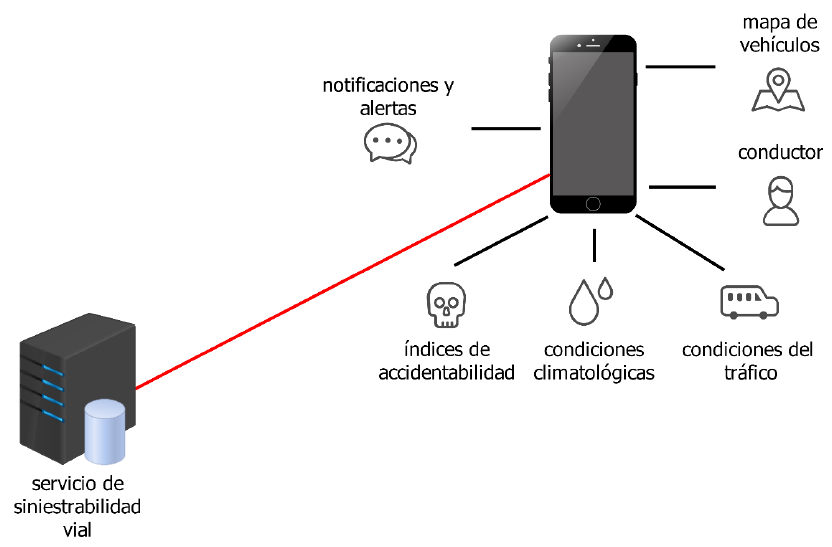
\includegraphics[width = 1\linewidth, height = 10.4cm]{Funcionalidad.png}
		\caption{Funcionalidades del Agente de Respuesta.}
		\label{Funcionalidad}
	\end{figure} \\
	\indent En la era digital actual, la nube se ha convertido en el pilar fundamental para el desarrollo y despliegue de aplicaciones y servicios. Amazon Web Services (AWS) se destaca como líder en el ámbito de servicios en la nube, ofreciendo una amplia gama de soluciones para empresas y desarrolladores. Este documento se centrará en el proceso de creación de servicios en AWS, para el Agente de Respuesta SIGOAVE, explorando los pasos esenciales para aprovechar al máximo la plataforma y proporcionar soluciones eficientes y escalables. \\\newline
	\indent La creación de servicios en AWS representa una respuesta a la creciente demanda de flexibilidad y eficiencia en el desarrollo de aplicaciones móviles y la gestión de infraestructuras. AWS ofrece una gama diversa de servicios, desde servicios de cómputo y almacenamiento hasta herramientas de inteligencia artificial y aprendizaje automático, permitiendo a los desarrolladores y empresas construir soluciones personalizadas y altamente escalables.
	
	\section{Objetivo}
	El objetivo principal al crear servicios en AWS es aprovechar la flexibilidad y la escalabilidad que la nube ofrece, permitiendo adaptarse rápidamente a las demandas cambiantes del mercado. Los servicios en la nube proporcionan una infraestructura sólida y confiable, reduciendo la carga operativa y permitiendo a los equipos enfocarse en la innovación en lugar de en la gestión de la infraestructura física. \\\newline
	\indent El proyecto incluye el diseño, desarrollo e implementación de un conjunto de agentes para gestión de accidentabilidad en vehículos. Los agentes propuestos pretenden mejorar los índices de accidentabilidad, disminuir los tiempos de respuesta para intervención y contribuir a evitar accidentes de tránsito. Los agentes poseerán autonomía de manera que podrán actuar en forma individual y conjunta por medio de mecanismos de retroalimentación para conseguir sistemas coordinados y actualizados. Estos medirán la probabilidad o grado de ocurrencia que un vehículo sufra un accidente de tránsito, y en base a esa información tomarán decisiones que disminuyan la probabilidad de que el accidente tome lugar. El sistema está formado por los agentes de adquisición, procesamiento y respuesta.
	\subsection{Objetivos Específicos}
	\begin{itemize}
		\item Agente de adquisición: es una aplicación móvil que recolectará información de un lector OBD, un receptor GPS, y otros sensores, y enviará información hacia un repositorio de datos en Internet.
		\item Agente de procesamiento: es una herramienta que usará computación en Internet, técnicas de minería de datos y algoritmos de aprendizaje de máquina para realizar la clasificación y procesamiento de la información almacenada en el repositorio de datos. El modelo de aprendizaje medirá la probabilidad o grado de ocurrencia que un vehículo sufra un accidente de tránsito.
		\item Agente de respuesta: es una aplicación móvil que permitirá a usuarios disponer de resultados (niveles de accidentabilidad), estadísticas y notificaciones.
	\end{itemize}
	
	\section{Esquema del Modelo de Agente}\label{Modelo_Agente}
	Se diseñó e implementó una aplicación móvil para Android basada en el lenguaje de programación Java. La aplicación interactúa con un escáner OBD2 y un receptor GPS para recoger parámetros y la ubicación del vehículo, y con un reloj inteligente para obtener el ritmo cardíaco del conductor. Una vez que la información es generada, se realiza la obtención de los parámetros de condiciones climáticas desde un servicio climatológico y el número de accidentes de tránsito dados cerca de una ubicación especifica desde una base de datos. En primera instancia, el agente de adquisición fue usado para generar el conjunto de datos de conducción denominada POLIDriving. Esta versión del conjunto de datos incluye información del conductor, del vehículo, condiciones climáticas y accidentes de tránsito. Una vez que el conjunto de datos fue generado, el agente de adquisición tiene la funcionalidad de recoger los parámetros y almacenarlos localmente. El agente de respuesta usará esta información para enviar al modelo y realizar predicciones. La Figura \ref{Esquema} presenta el esquema de funcionamiento del agente de adquisición.
	\begin{figure}[!h]
		\centering
		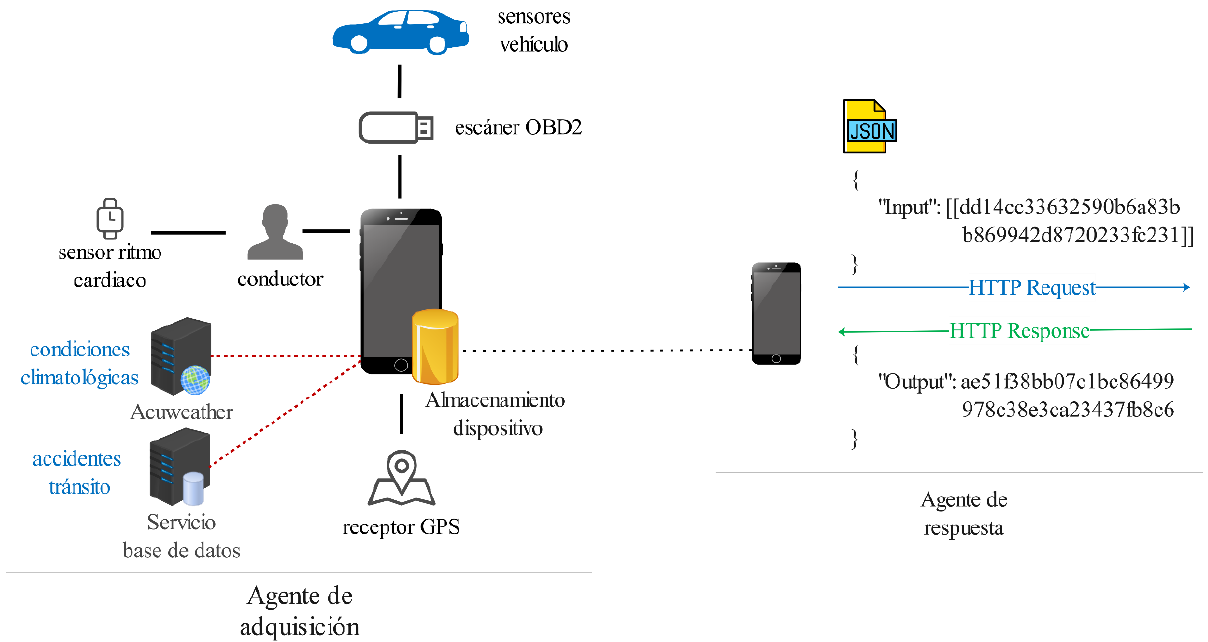
\includegraphics[width = 1\linewidth, height = 9.9cm]{Esquema.png}
		\caption{Esquema de Funcionamiento del Agente de Adquisición.}
		\label{Esquema}
	\end{figure} \\
	\indent El artículo \cite{marcillo2022systematic} y publicado en Applied Sciences (Q2), proporcionó información relacionada a fuentes de datos y atributos usados por los modelos de predicción, y a plataformas, servicios de Internet y simuladores usados para recolectar información. Esta información permitió diseñar e implementar un agente de adquisición que se ajuste a ciertos requerimientos funcionales y no funcionales. En el siguiente enlace se encuentra el conjunto de datos POLIDriving:
	\begin{itemize}
		\item \textcolor{blue}{\url{https://github.com/laboratorioAI/PIS_20_02_AGENTES_IA/tree/main/Actualizacion_2024/Dataset}}
	\end{itemize}
	
	\section{Implementación Servicios AWS}
	El agente de procesamiento consta de 2 fases:
	\begin{itemize}
		\item Creación, entrenamiento e implementación del modelo de aprendizaje de máquina.
		\item Configuración y despliegue del API REST para consultar en tiempo real el nivel de riesgo de sufrir un accidente de tránsito.
	\end{itemize}
	\indent\indent Para la primera fase se creó, entrenó, e implementó un modelo usando el servicio SageMaker de Amazon Web Services (AWS). Mientras que para la segunda fase se configuró y desplegó un API REST usando los servicios SageMaker, Lambda, API Gateway y S3 de AWS. La Figura \ref{Infraestructura} presenta el esquema de infraestructura usado por el agente de procesamiento.
	\begin{figure}[!h]
		\centering
		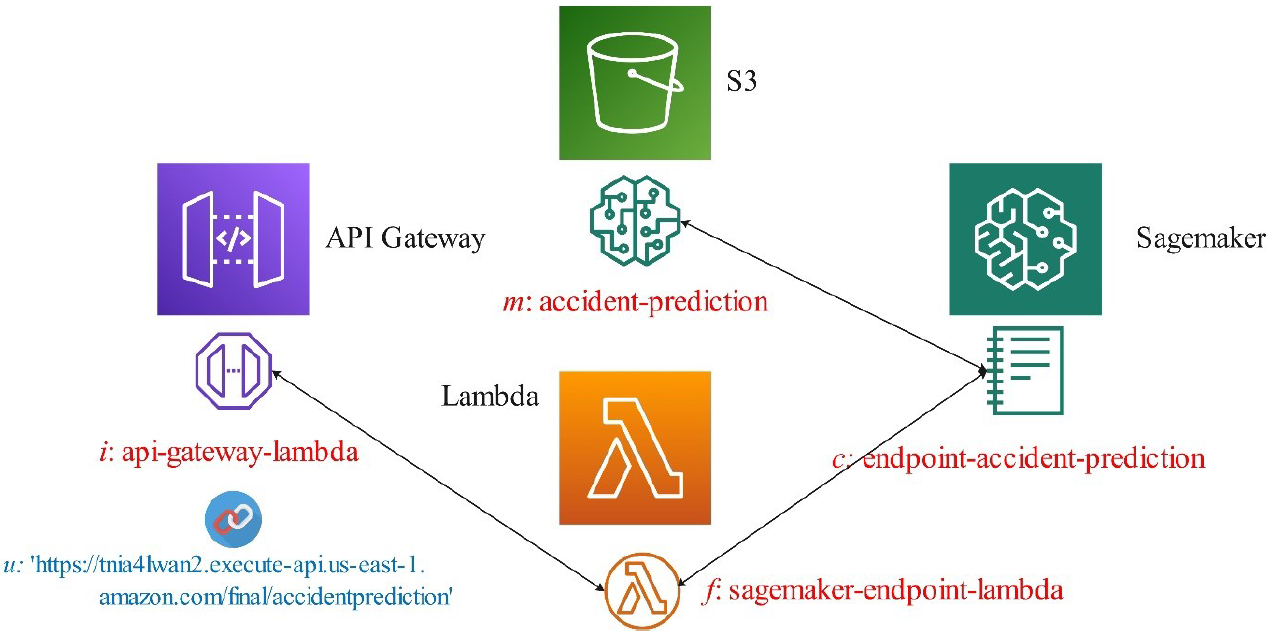
\includegraphics[width = 1\linewidth, height = 9.8cm]{Infraestructura.png}
		\caption{Infraestructura del agente de procesamiento.}
		\label{Infraestructura}
	\end{figure}
	\subsection{Administración de Identidades - AWS IAM}\label{AWS_IAM}
	El primer paso para la creación de los servicios en AWS, es la creación de la ``Identidad de Usuario'', mediante el uso del Administrador de Identidades. Con AWS Identity and Access Management (IAM), puede especificar quién o qué puede acceder a los servicios y recursos en AWS, administrar de forma centralizada los permisos específicos y analizar el acceso para perfeccionar los permisos en todo AWS \cite{IAM}. La Figura \ref{Funcionamiento_IAM} muestra el funcionamiento de IAM.
	\begin{figure}[!h]
		\centering
		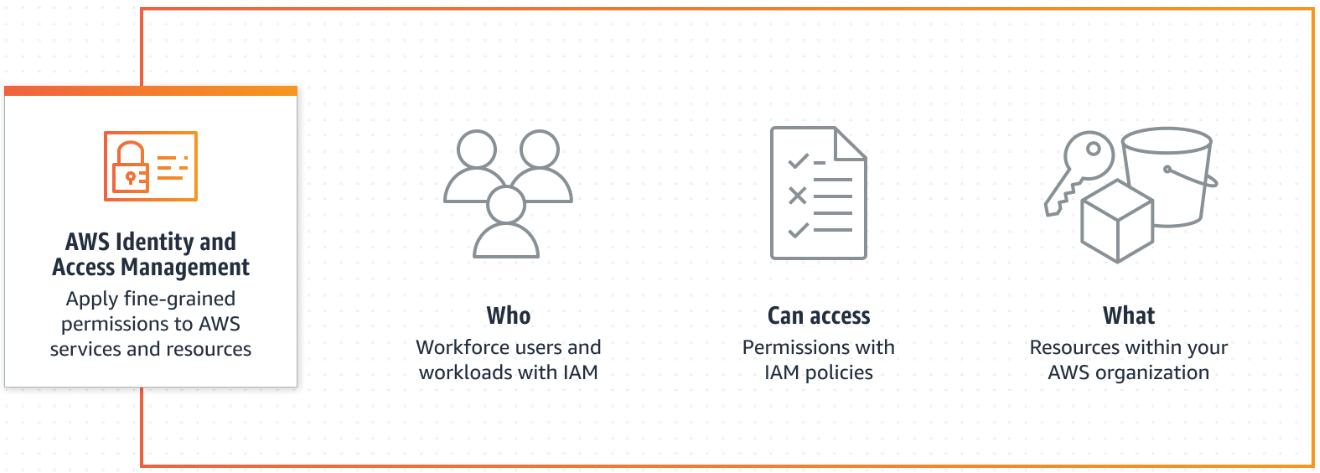
\includegraphics[width = 1\linewidth, height = 8.5cm]{Funcionamiento_IAM.png}
		\caption{Cómo funciona la gestión de acceso e identidad de AWS.}
		\label{Funcionamiento_IAM}
	\end{figure} \\
	\indent Para la creación de una nueva identidad es necesario dirigirse a la consola de AWS y buscar el servicio de IAM como muestra la Figura \ref{Servicio_IAM}, una vez localizado el servicio se ingresa al mismo y se puede apreciar el panel de control de IAM.
	\begin{figure}[!h]
		\centering
		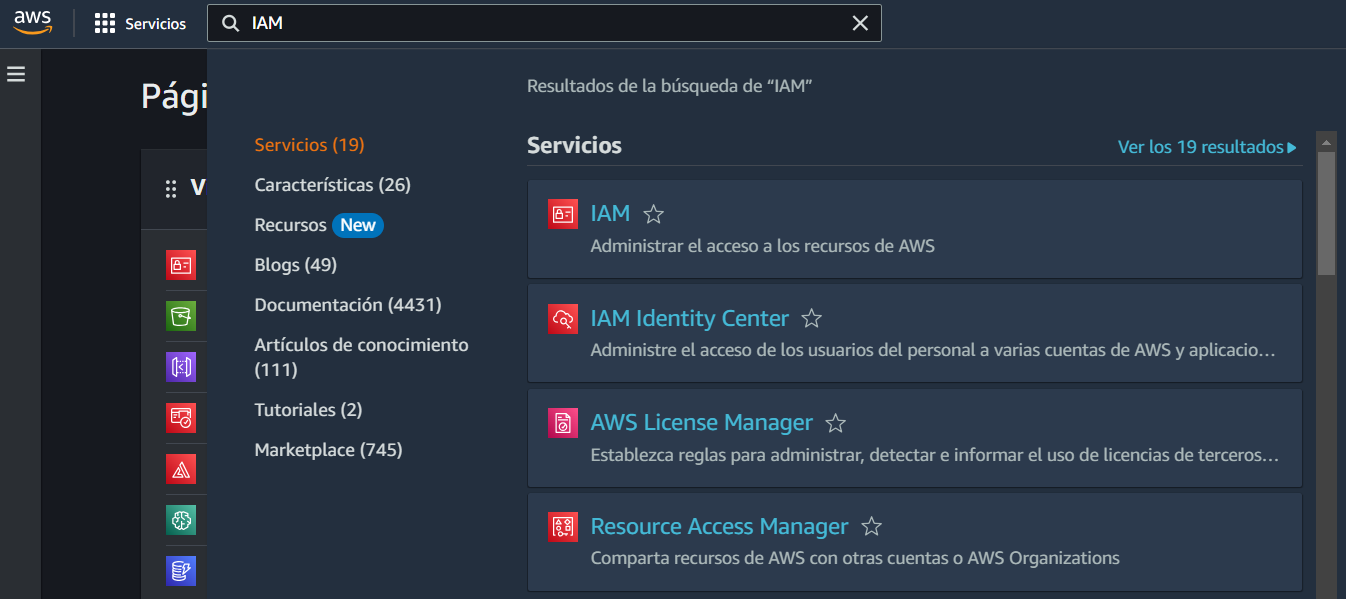
\includegraphics[width = 1\linewidth, height = 8.5cm]{Servicio_IAM.png}
		\caption{Búsqueda Servicio IAM.}
		\label{Servicio_IAM}
	\end{figure} \\
	\indent En el panel de control de IAM se localiza la opción ``Usuarios'' como muestra la Figura \ref{Usuarios_IAM}. Se ingresa a este dando ``Clic'' sobre el número, en un principio este cera 0, esto llevara a una nueva pantalla en la que se podrá crear un nuevo usuario como muestra la Figura \ref{Crear_Usuario_IAM}.
	\begin{figure}[!h]
		\centering
		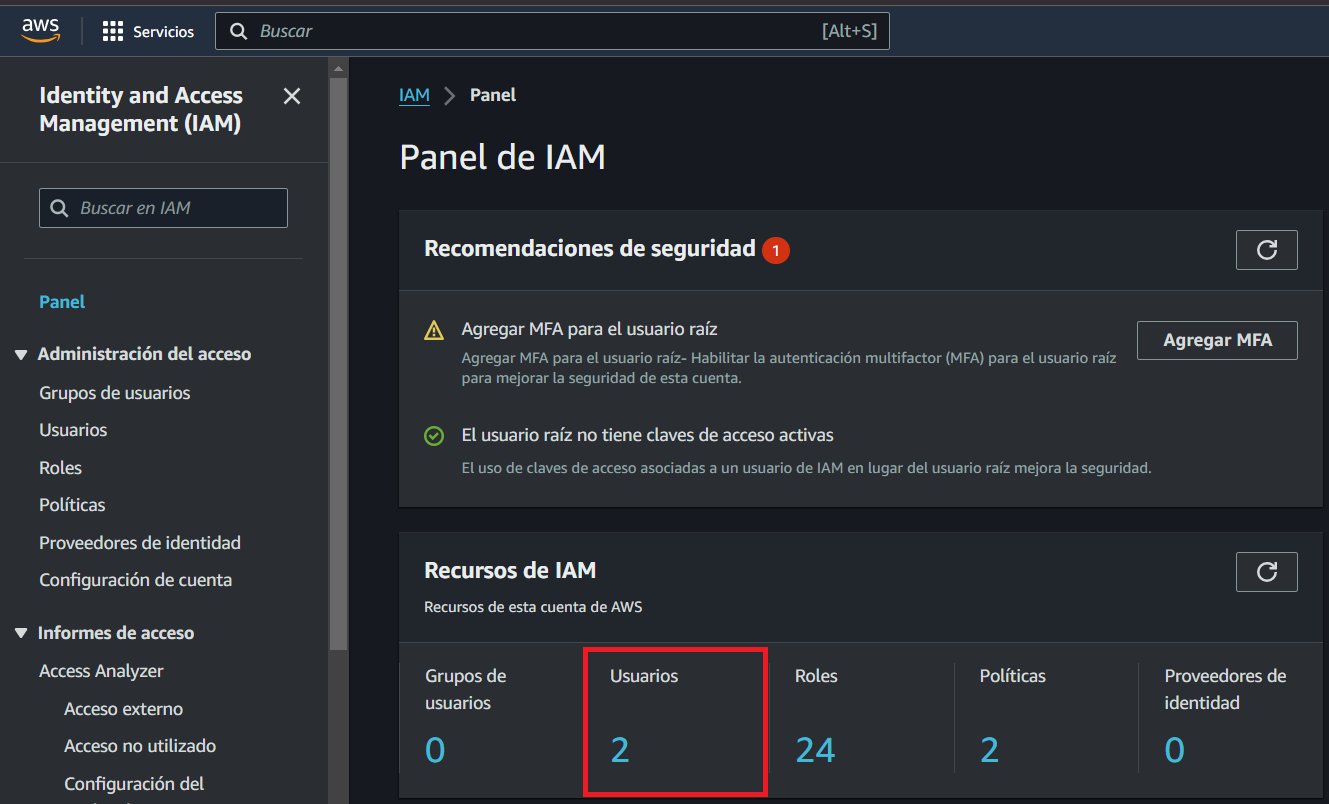
\includegraphics[width = 1\linewidth, height = 8.2cm]{Usuarios_IAM.png}
		\caption{Usuarios IAM.}
		\label{Usuarios_IAM}
	\end{figure}
	\begin{figure}[!h]
		\centering
		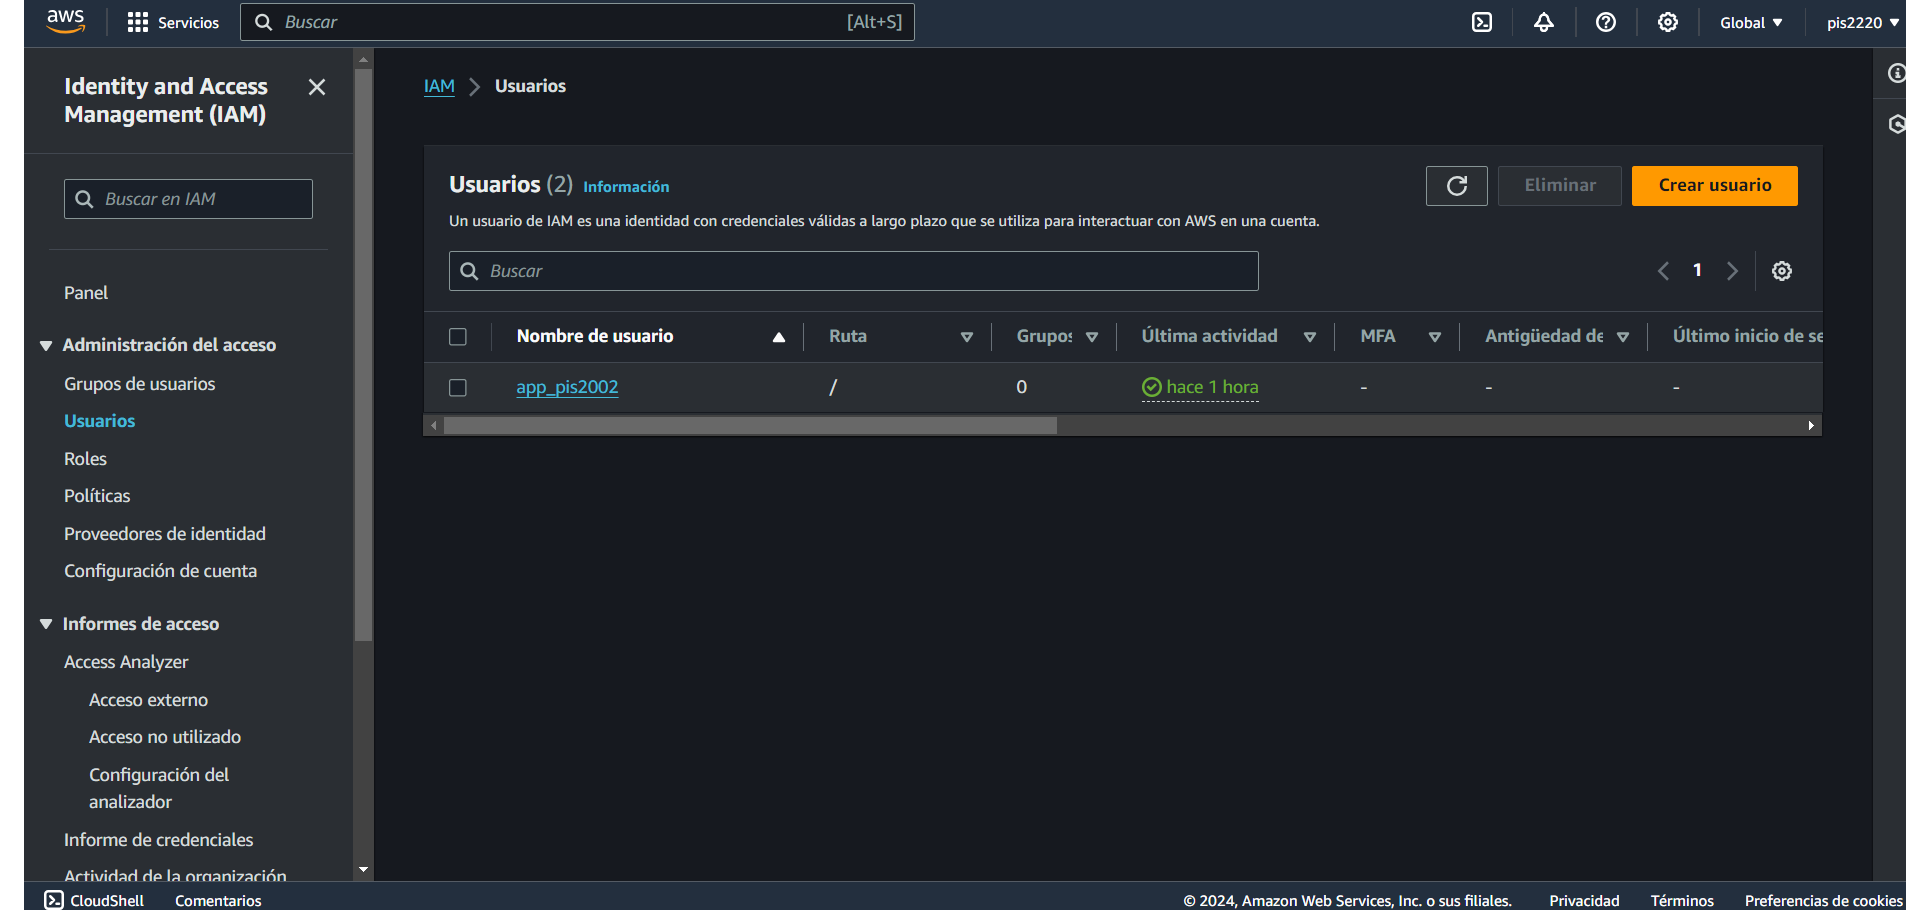
\includegraphics[width = 1\linewidth, height = 8.2cm]{Crear_Usuario_IAM.png}
		\caption{Crear Usuario IAM.}
		\label{Crear_Usuario_IAM}
	\end{figure} \\
	\indent En la siguiente pantalla se debe ingresar un nombre de usuario, este nombre debe ser único y reconocible; posteriormente, se debe dar ``Clic''en el botón ``Siguiente'' como muestra la Figura \ref{Nombre_Usuario}. Esto redirigirá a una nueva pantalla donde se podrá escoger las políticas que se desee dar al usuario, para ello se escoge la opción ``Adjuntar políticas directamente''. Podemos escoger cuantas políticas deseemos, ver Figura \ref{Permisos_Usuario_IAM}. En futuro se pueden agregar más políticas de ser necesario.
	\begin{figure}[!h]
		\centering
		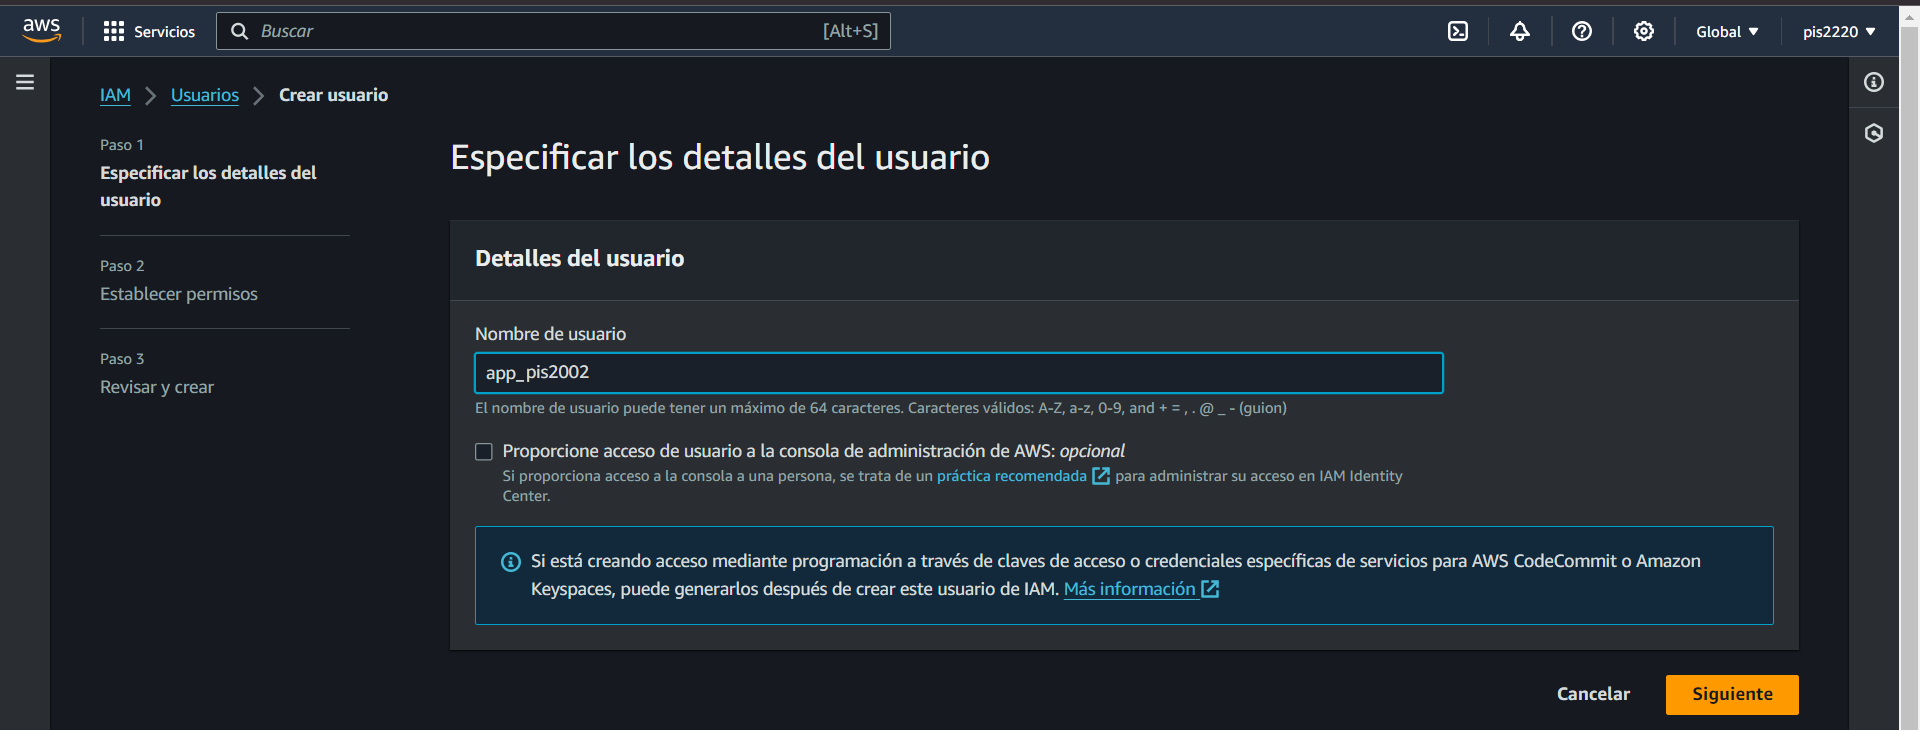
\includegraphics[width = 1\linewidth, height = 7.6cm]{Nombre_Usuario.png}
		\caption{Nombre de Usuario IAM.}
		\label{Nombre_Usuario}
	\end{figure}
	\begin{figure}[!h]
		\centering
		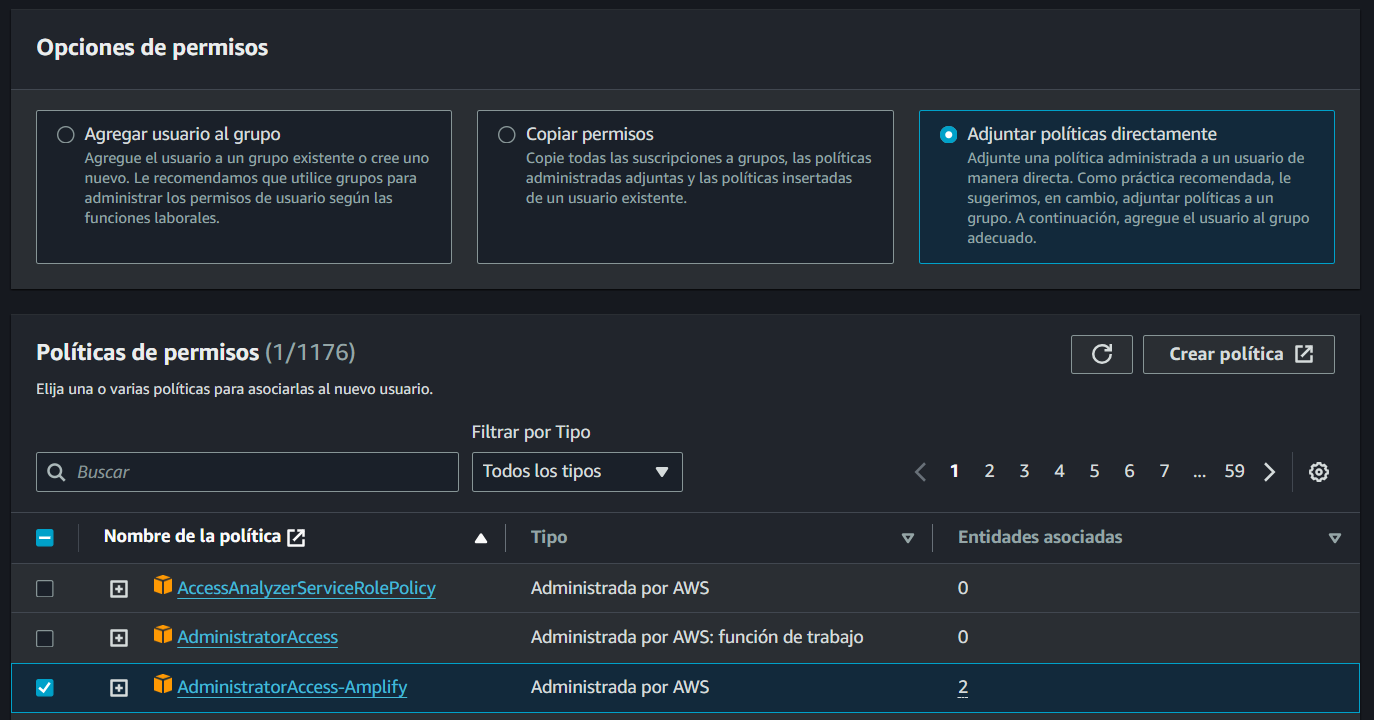
\includegraphics[width = 1\linewidth, height = 7.6cm]{Permisos_Usuario_IAM.png}
		\caption{Permisos Usuario IAM.}
		\label{Permisos_Usuario_IAM}
	\end{figure} \\
	\indent Tras agregar las políticas deseadas al usuario, se pasa a una nueva interfaz donde se muestra un resumen de las políticas tomadas para el usuario. Ver Figura \ref{Resumen_Permisos_IAM}.
	\begin{figure}[!h]
		\centering
		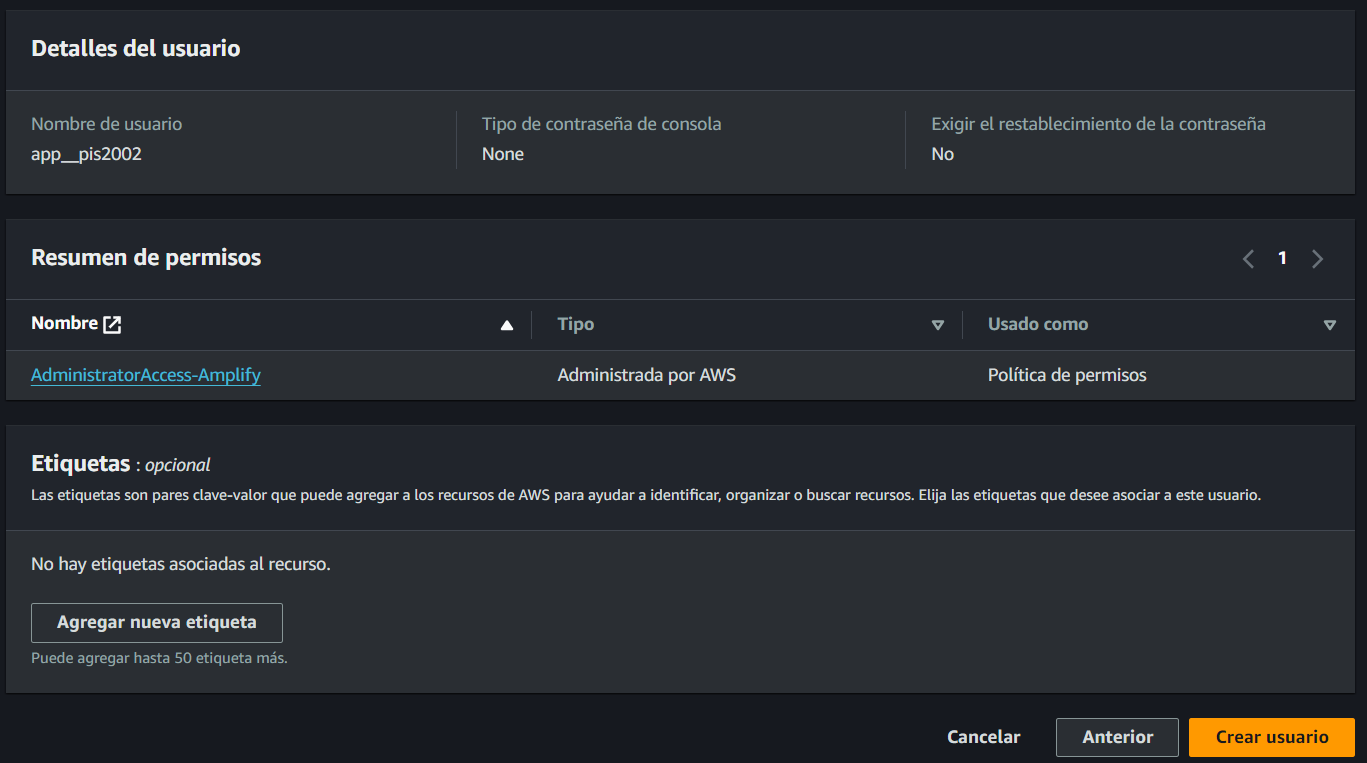
\includegraphics[width = 1\linewidth, height = 7.8cm]{Resumen_Permisos_IAM.png}
		\caption{Resumen Permisos IAM.}
		\label{Resumen_Permisos_IAM}
	\end{figure} \\
	\indent Finalmente, se crea el usuario presionando en el botón ``Crear Usuario'', tras lo cual se redirigirá a la consola de IAM. En la consola se puede apreciar que el usuario a sido creado con exito. Ver Figura \ref{Usuario_IAM_Creado}.
	\begin{figure}[!h]
		\centering
		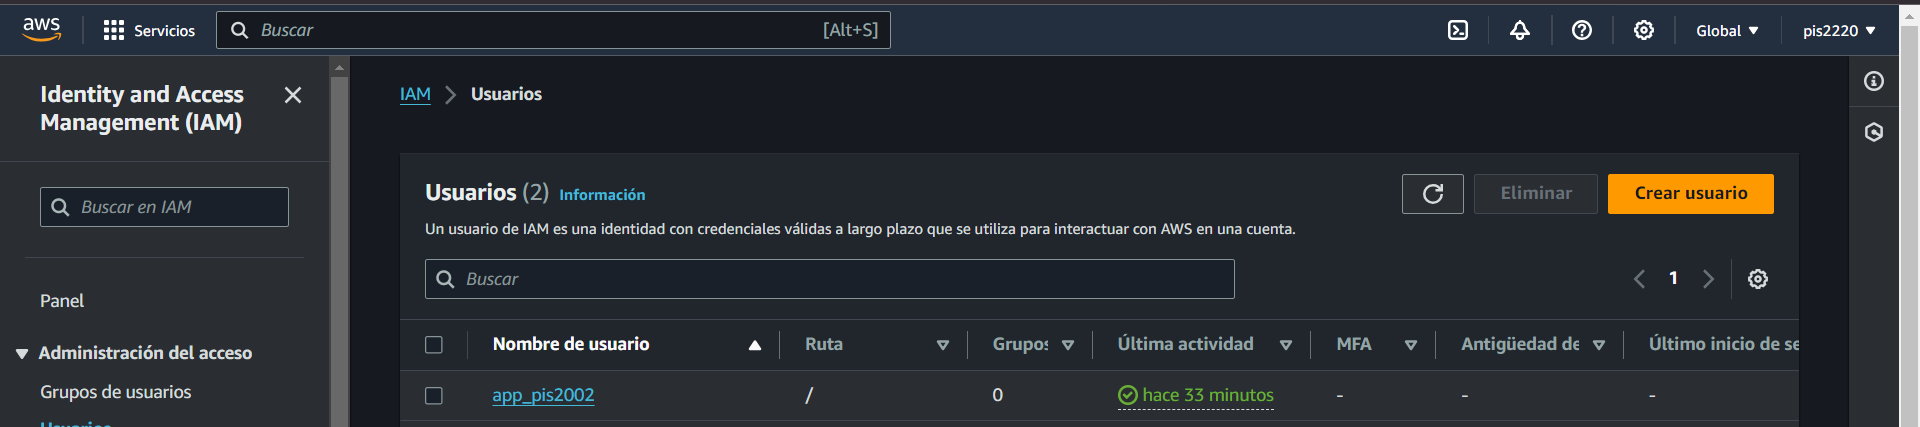
\includegraphics[width = 1\linewidth, height = 7.8cm]{Usuario_IAM_Creado.png}
		\caption{Usuario IAM Creado.}
		\label{Usuario_IAM_Creado}
	\end{figure} \\
	\indent Creado el usuario, ingresamos al mismo dando ``Clic'' sobre el nombre del usuario y se muestra un resumen detallado de las características del usuario, ver Figura \ref{Detalle_Usuario_IAM}. En esta página se tiene que seleccionar la opción ``Credenciales de seguridad'', dentro de ``Credenciales de seguridad'' se busca la opción ``Claves de acceso'' y se crea una nueva clave de acceso dando ``Clic'' sobre el botón ``Crear clave de acceso'', Ver Figura \ref{Clave_Acceso_IAM}
	\begin{figure}[!h]
		\centering
		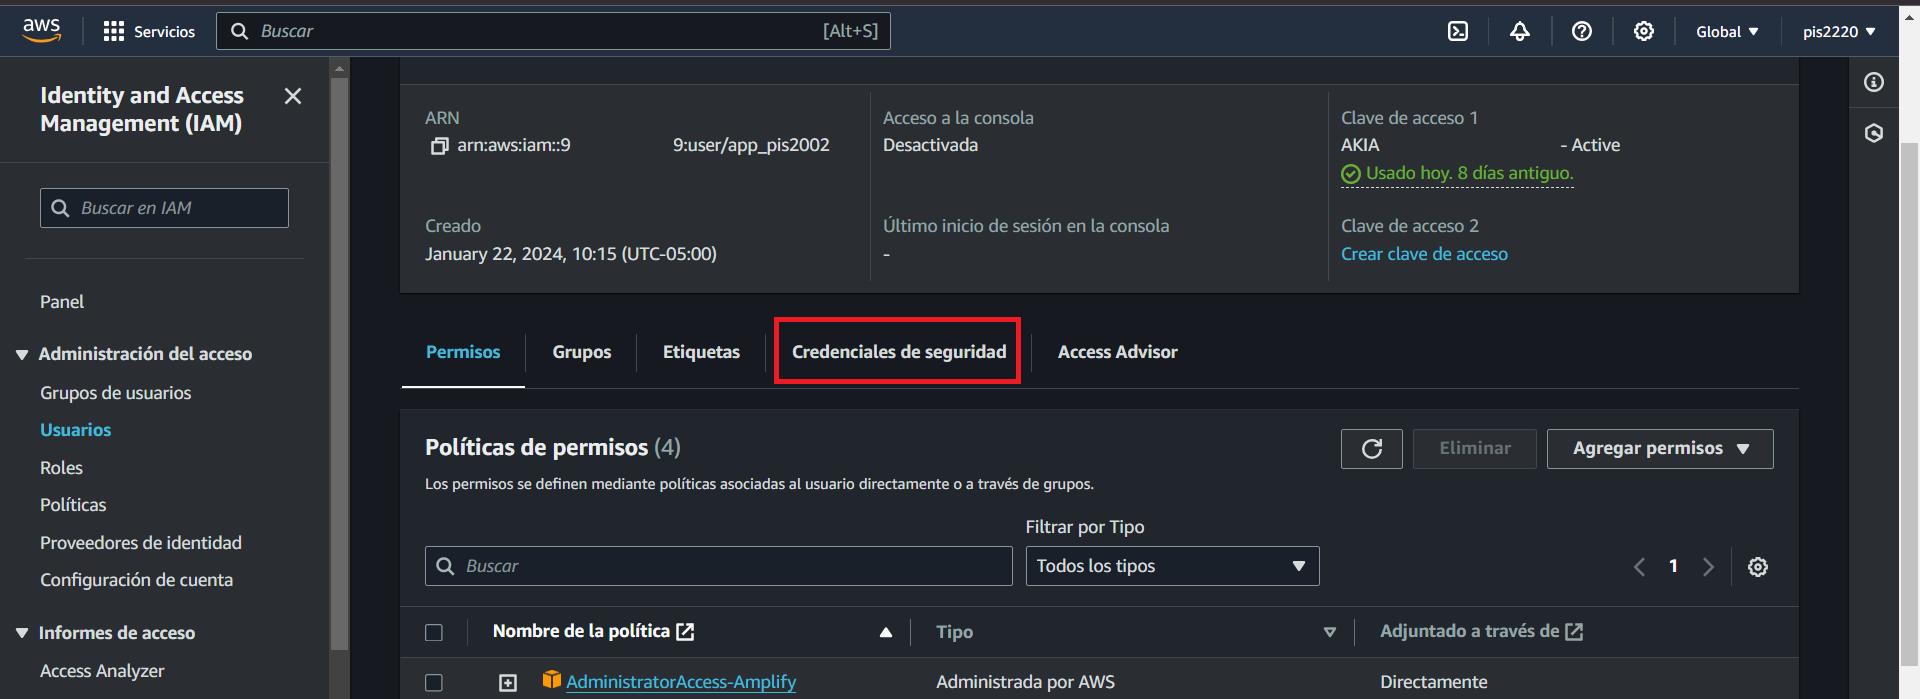
\includegraphics[width = 1\linewidth, height = 7.8cm]{Detalle_Usuario_IAM.png}
		\caption{Detalle Usuario IAM.}
		\label{Detalle_Usuario_IAM}
	\end{figure}
	\begin{figure}[!h]
		\centering
		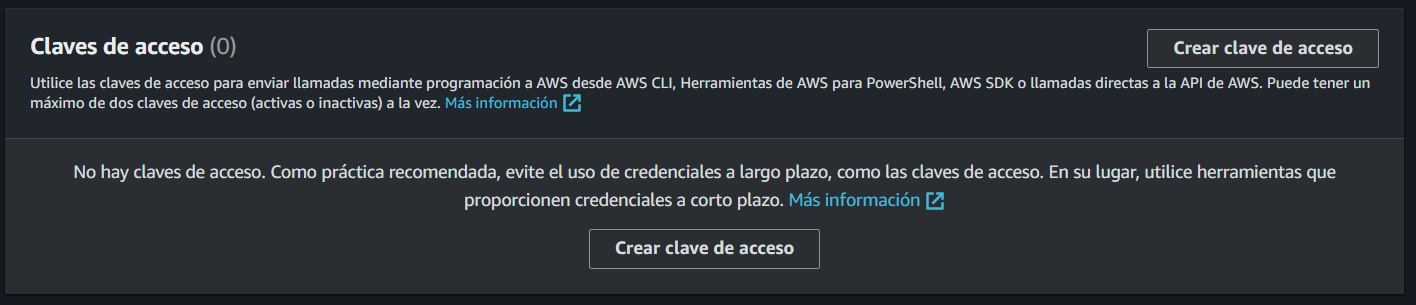
\includegraphics[width = 1\linewidth, height = 7.8cm]{Clave_Acceso_IAM.png}
		\caption{Clave de Acceso IAM.}
		\label{Clave_Acceso_IAM}
	\end{figure} \\
	\indent En la siguiente ventana se selecciona ``Interfaz de línea de comandos (CLI)'' y ``Entiendo la recomendación anterior y deseo proceder a la creación de una clave de acceso'' como se aprecia en la Figura \ref{CLI_IAM}.
	\begin{figure}[!h]
		\centering
		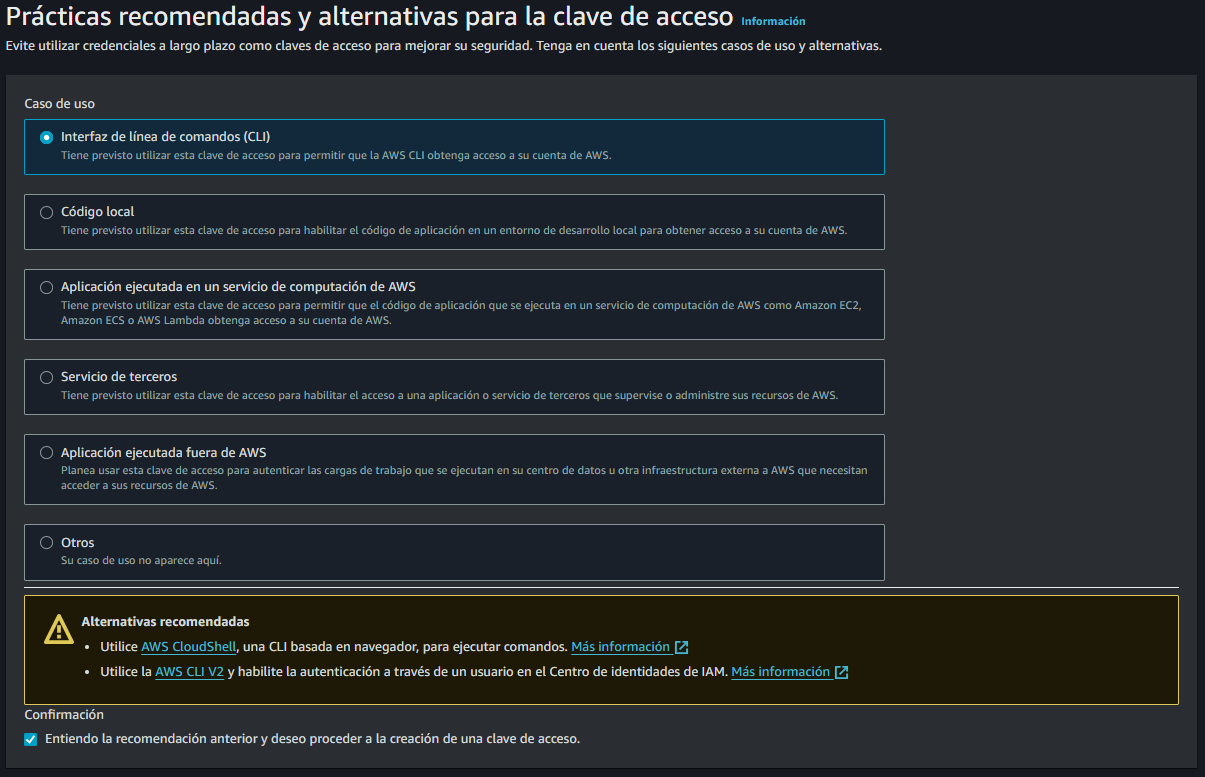
\includegraphics[width = 1\linewidth, height = 7.4cm]{CLI_IAM.png}
		\caption{Casos de uso IAM.}
		\label{CLI_IAM}
	\end{figure} \\
	\indent Agregamos una descripción a la clave y posteriormente se  muestra la clave creada. En la Figura \ref{Access_Secret_Key_IAM} se muestra la clave de acceso creada, en ella se aprecia que se crearon dos claves: ``Clave de acceso'' y ``Clave de acceso secreta''.  Se debe recordar almacenar esta información en un lugar segura ya que en futuro no se podrá acceder a esta información.
	\begin{figure}[!h]
		\centering
		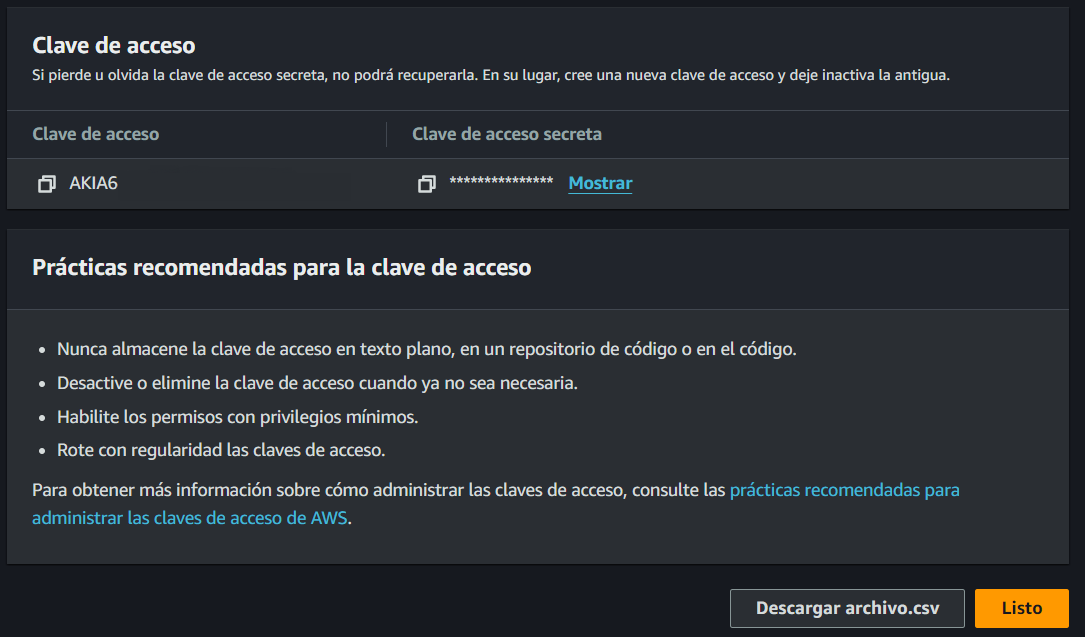
\includegraphics[width = 1\linewidth, height = 7.4cm]{Access_Secret_Key_IAM.png}
		\caption{Access y Secret Key IAM.}
		\label{Access_Secret_Key_IAM}
	\end{figure} \\
	\indent Finalmente, al presionar ``Listo'' en la pantalla anterior se regresa a la pantalla principal. En esta pantalla se muestra un resumen detalla de las nuevas ``Clases de acceso'' y ver si esta activa o no. Ver Figura \ref{Detalle_Clave_IAM}.
	\begin{figure}[!h]
		\centering
		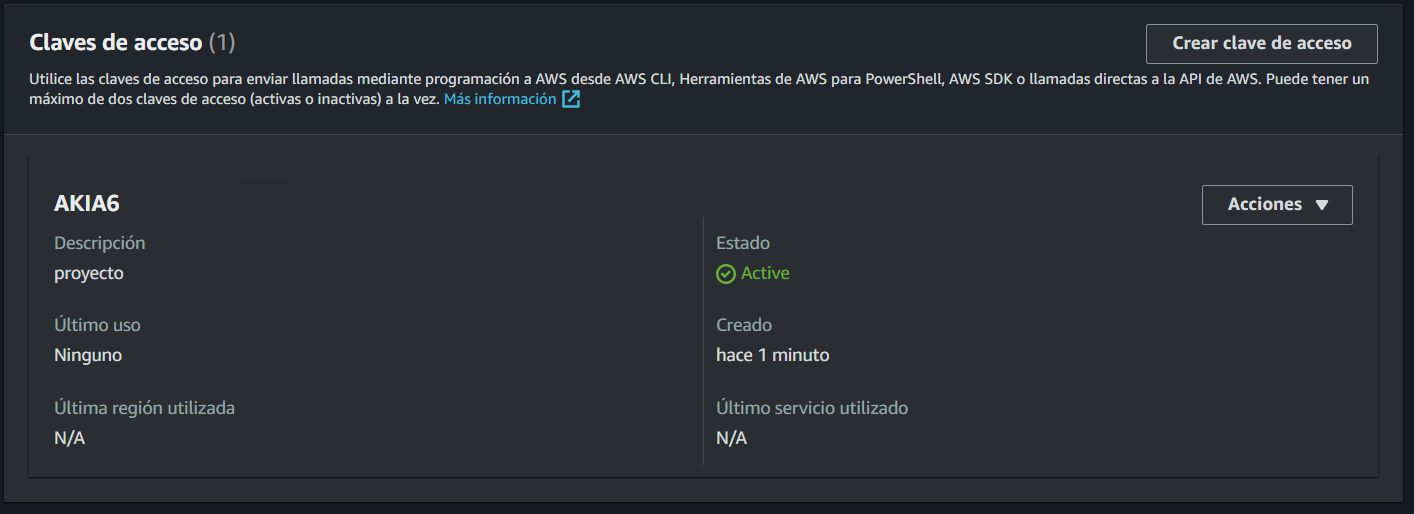
\includegraphics[width = 1\linewidth, height = 6.5cm]{Detalle_Clave_IAM.png}
		\caption{Detalles de Claves de Acceso.}
		\label{Detalle_Clave_IAM}
	\end{figure}
	\subsection{Machine Learning Service - AWS SageMaker}\label{AWS_SageMaker}
	El siguiente paso es la implementación del modelo en ``SageMaker'' de AWS. Amazon SageMaker es un servicio de aprendizaje automático totalmente gestionado. SageMaker permite a los desarrolladores y a los analistas de datos crear y perfeccionar modelos de aprendizaje automático de forma rápida y sencilla y, a continuación, implementarlos directamente en un entorno alojado listo para su uso \cite{SageMaker}. En la Figura \ref{Funcionamiento_SageMaker} se aprecia el funcionamiento de SageMaker.
	\begin{figure}[!h]
		\centering
		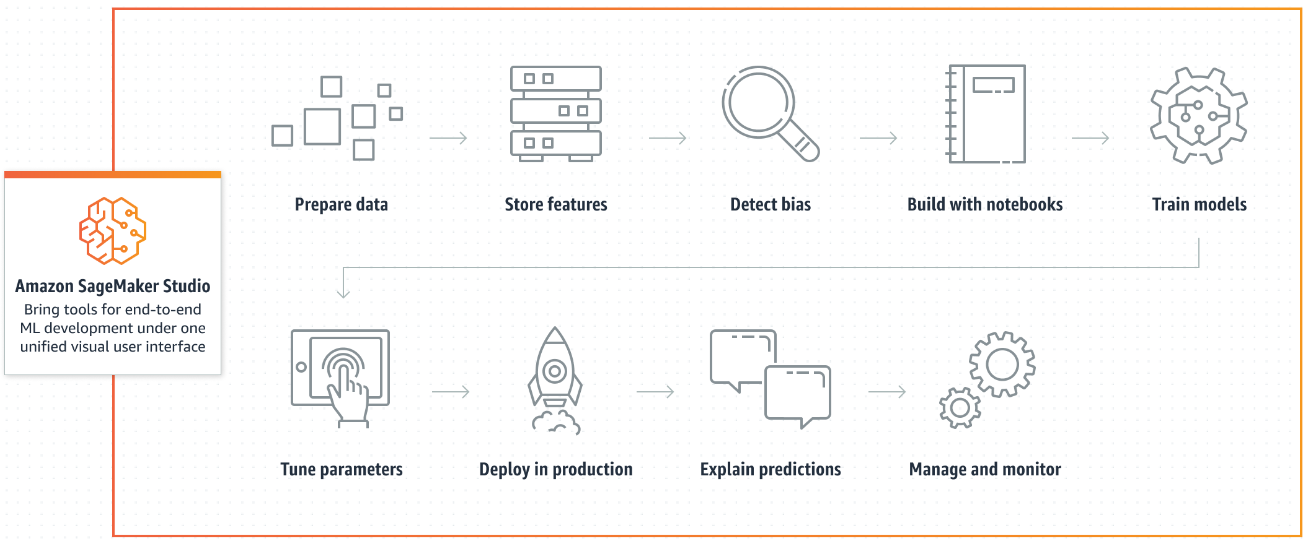
\includegraphics[width = 1\linewidth, height = 6.6cm]{Funcionamiento_SageMaker.png}
		\caption{Funcionamiento de SageMaker.}
		\label{Funcionamiento_SageMaker}
	\end{figure} \\
	\indent Antes de empezar con la configuración de SageMaker con el usuario con el cual se va a trabajar es necesario agregar una nueva política llamada ``AdministratorAccess``, para ello como se menciona en el apartado \ref{AWS_IAM} en los detalles del usuario se puede agregar nuevas políticas, ver Figura \ref{Nueva_Politica_SageMaker}.
	\begin{figure}[!h]
		\centering
		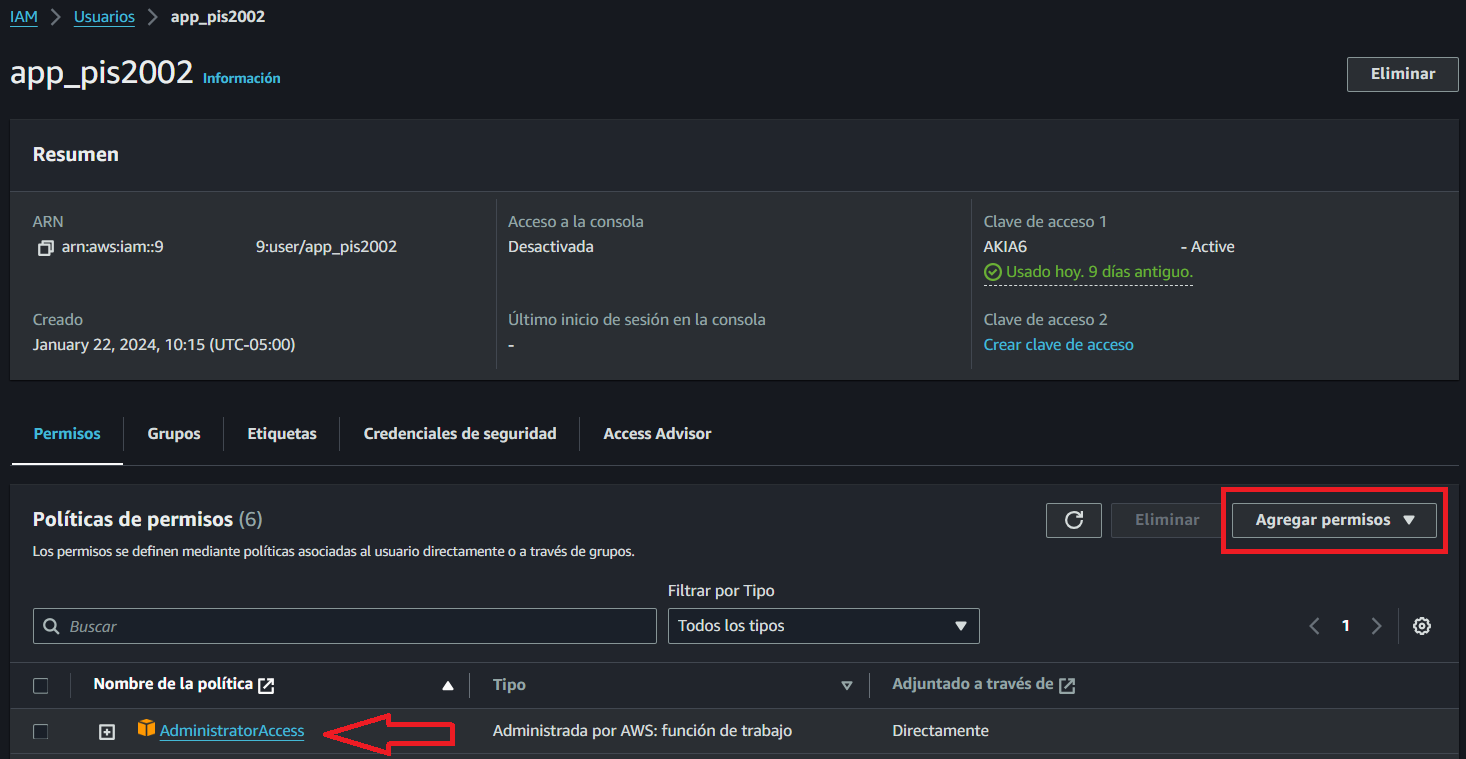
\includegraphics[width = 1\linewidth, height = 7.2cm]{Nueva_Politica_SageMaker.png}
		\caption{Agregación Nueva Política.}
		\label{Nueva_Politica_SageMaker}
	\end{figure} \\
	 \indent Adicionalmente, es necesario tener un ``DataSet'' con extensión ``CSV'' con el cual se va a trabajar. Este archivo se encuentra en la dirección URL mencionada en el apartado \ref{Modelo_Agente}, de los diferentes archivos de datos que se encuentra se usar DataSet cuyo etiqueta es ``20221215\_151443\_pre'', en la Figura \ref{Dataset_Sagemaker} se muestra una parte del contenido del mencionado DataSet.
	\begin{figure}[!h]
		\centering
		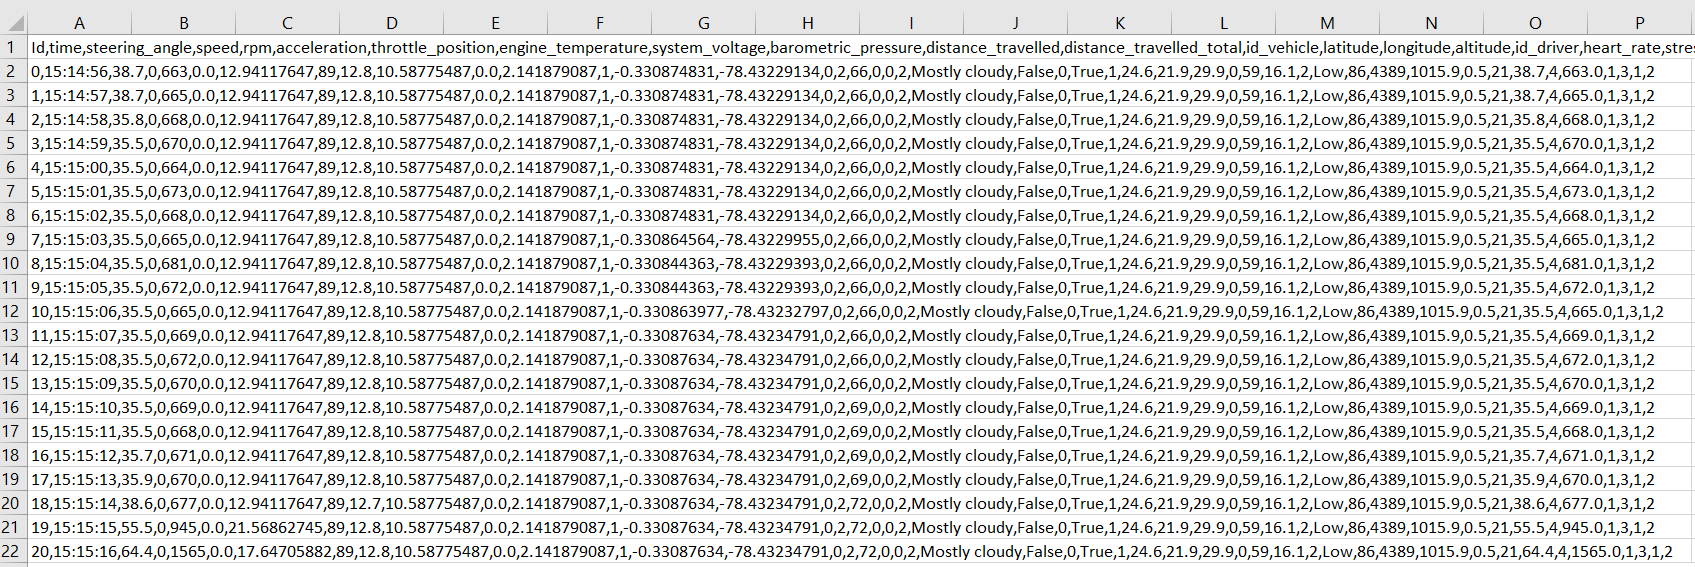
\includegraphics[width = 1\linewidth, height = 7.2cm]{Dataset_Sagemaker.png}
		\caption{Parte de Contenido DataSet.}
		\label{Dataset_Sagemaker}
	\end{figure} \\
	\indent Para la creación de este servicio es necesario dirigirse a la consola de AWS y buscar el servicio de SageMaker como muestra la Figura \ref{Servicio_SageMaker}, una vez localizado el servicio se ingresa al mismo y se puede apreciar el panel de control. En el panel de control localizamos la opción ``Bloc de Notas'' y dentro de esta opción localizamos ``Instancias de bloc de notas'' como muestra la Figura \ref{Nootebook_SageMaker}.
	\begin{figure}[!h]
		\centering
		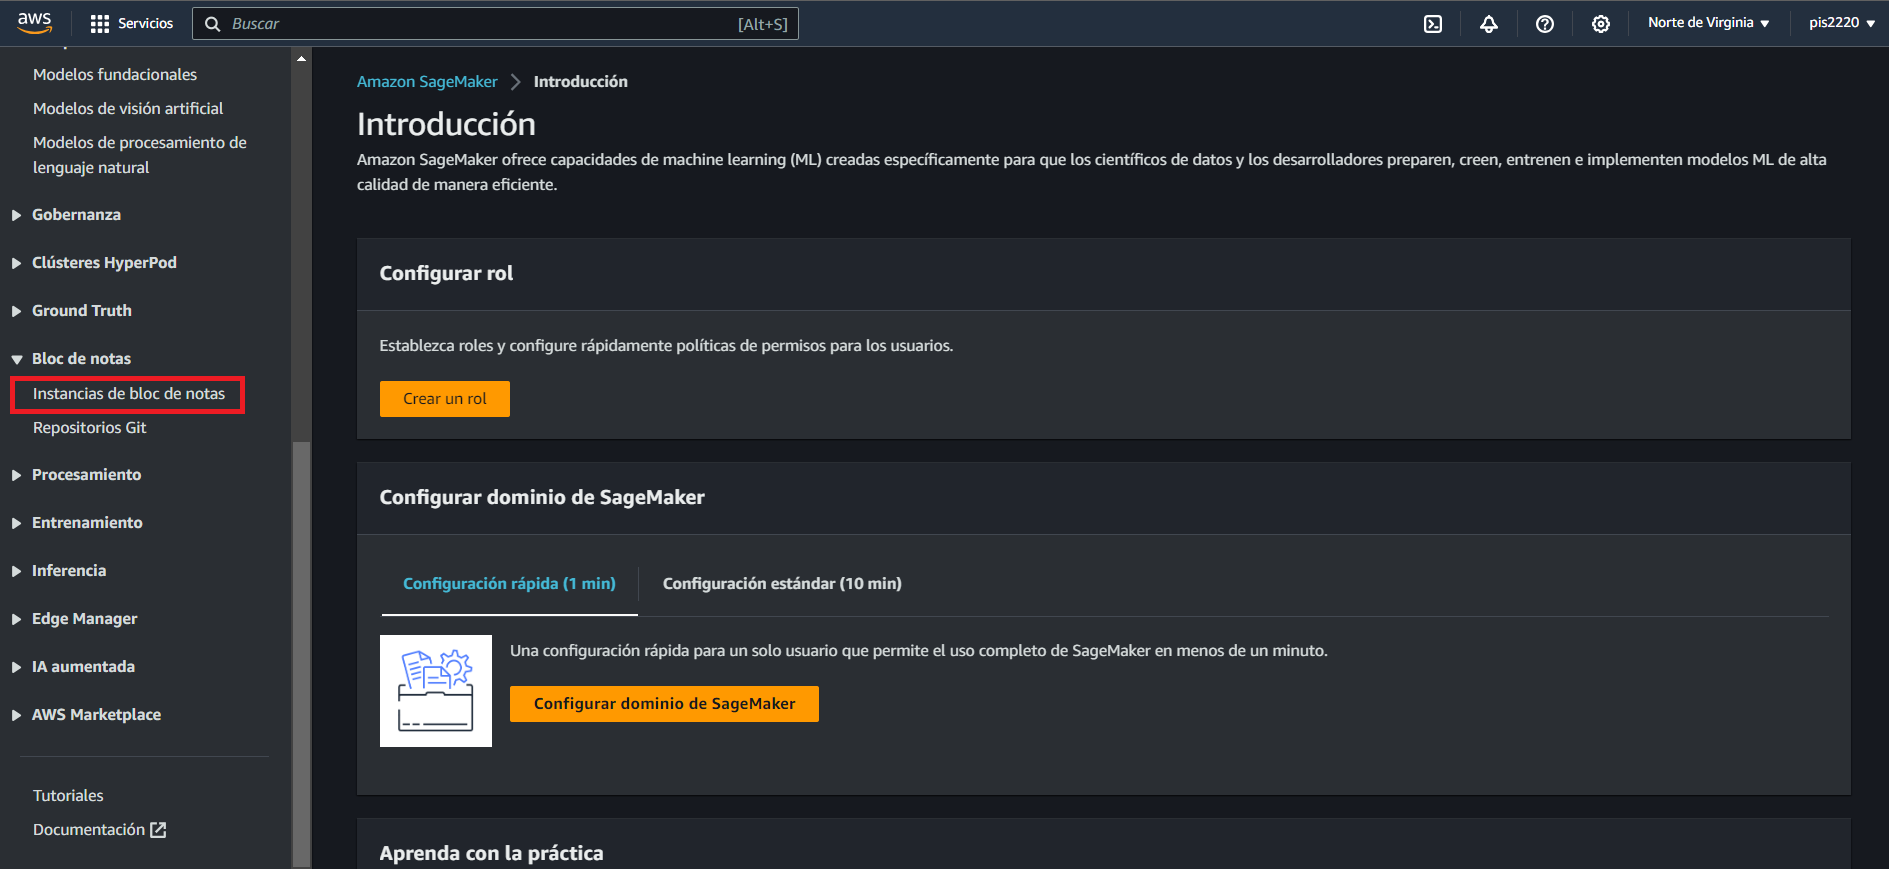
\includegraphics[width = 1\linewidth, height = 6.7cm]{Nootebook_SageMaker.png}
		\caption{Búsqueda NoteBook de SageMaker.}
		\label{Nootebook_SageMaker}
	\end{figure} \\
	\indent Al ingresar al panel de ``Instancias de bloc de notas'' se puede crear una nueva instancia tan solo con dar ``Clic'' en el botón de ``Crear instancia de bloc de notas'' como muestra la Figura \ref{Instancias_SageMaker}. Al hacer esto redirigirá a un nuevo formulario.
	\begin{figure}[!h]
		\centering
		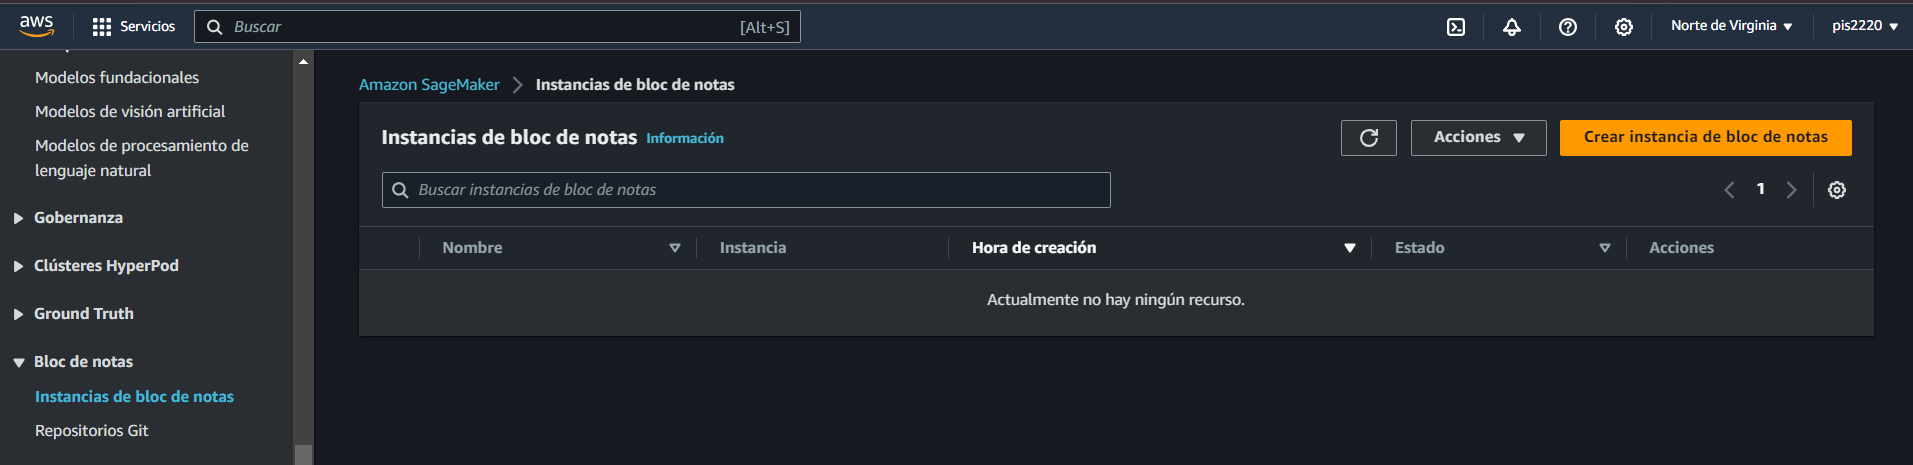
\includegraphics[width = 1\linewidth, height = 6.7cm]{Instancias_SageMaker.png}
		\caption{Crear NoteBook de SageMaker.}
		\label{Instancias_SageMaker}
	\end{figure} \\
	\indent En la página ``Crear instancia de bloc de notas'', en el cuadro de Configuración de la instancia de bloc de notas, se rellena los siguientes campos:
	\begin{itemize}
		\item El Nombre de la instancia.
		\item En Tipo de instancia: ml.t2.medium.
		\item En Inferencia elástica, mantener la selección predeterminada.
		\item En Identificador de plataforma, mantener la selección predeterminada.
	\end{itemize}
	\indent \indent La Figura \ref{Configuracion_Instancia_SageMaker} muestra las diferentes configuraciones realizadas.
	\begin{figure}[!h]
		\centering
		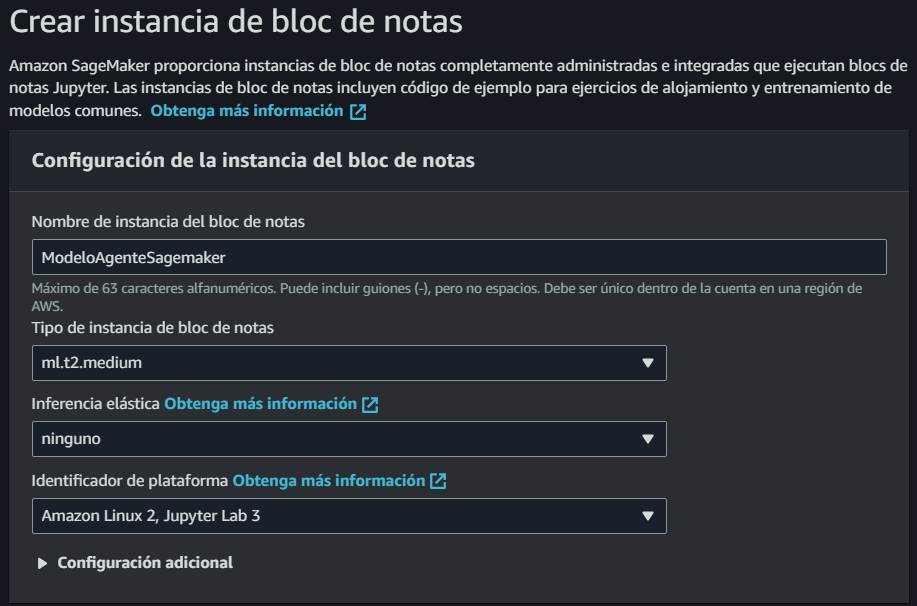
\includegraphics[width = 1\linewidth, height = 6.4cm]{Configuracion_Instancia_SageMaker.png}
		\caption{Configuración de la instancia del bloc de notas.}
		\label{Configuracion_Instancia_SageMaker}
	\end{figure} \\
	\indent Una vez realizada la configuración de la instancia del bloc de notas, se procede a configurar los ``Permisos y cifrado''. En la sección Permisos y cifrado, para el rol de IAM, se selecciona ``Crear un nuevo rol'' como muestra la Figura \ref{Permisos_Cifrado_SageMaker} y, en el cuadro de diálogo ``Crear una función de IAM'', seleccione ``Cualquier bucket S3'' y seleccionar ``Crear rol'' como muestra la Figura \ref{Crear_Función_IAM}.
	\begin{figure}[!h]
		\centering
		\includegraphics[width = 1\linewidth, height = 6.4cm]{Crear_Función_IAM.png}
		\caption{Crear una función de IAM.}
		\label{Crear_Función_IAM}
	\end{figure} \\
	\indent Amazon SageMaker creará el rol AmazonSageMaker-ExecutionRole. Ver Figura \ref{SageMaker_ExecutionRole}.
	\begin{figure}[!h]
		\centering
		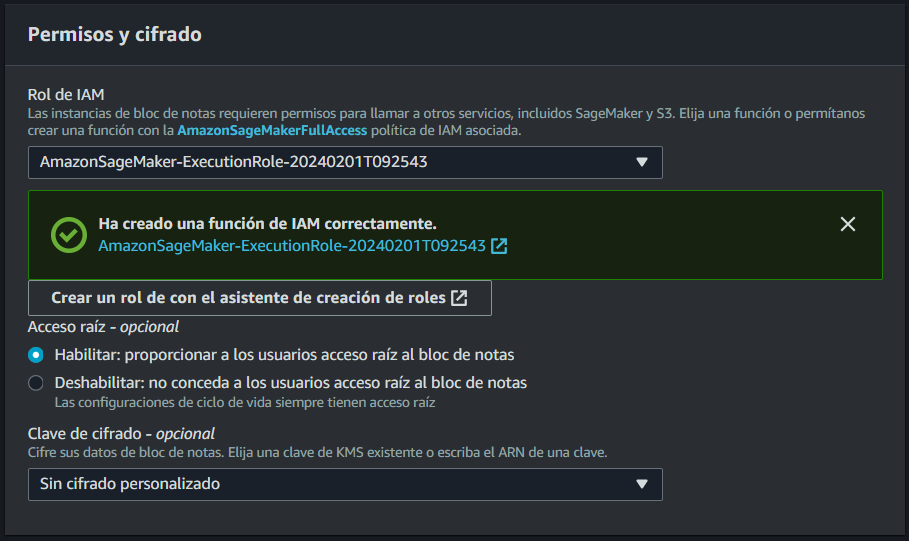
\includegraphics[width = 1\linewidth, height = 7.6cm]{SageMaker_ExecutionRole.png}
		\caption{SageMaker ExecutionRole.}
		\label{SageMaker_ExecutionRole}
	\end{figure} \\
	\indent Conservar la configuración predeterminada para las demás opciones y elegir ``Crear instancia de bloc de notas''. En la sección Instancias de bloc de notas, se muestra la instancia de cuaderno recién creada con un estado ``Pendiente'', ver Figura \ref{Instancia_Creada_SageMaker}. El cuaderno estará listo cuando el estado cambie a ``En Servicio'' lo cual puede tardar varios minutos, ver Figura \ref{Instancia_Creada_SageMaker_Online}.
	\begin{figure}[!h]
		\centering
		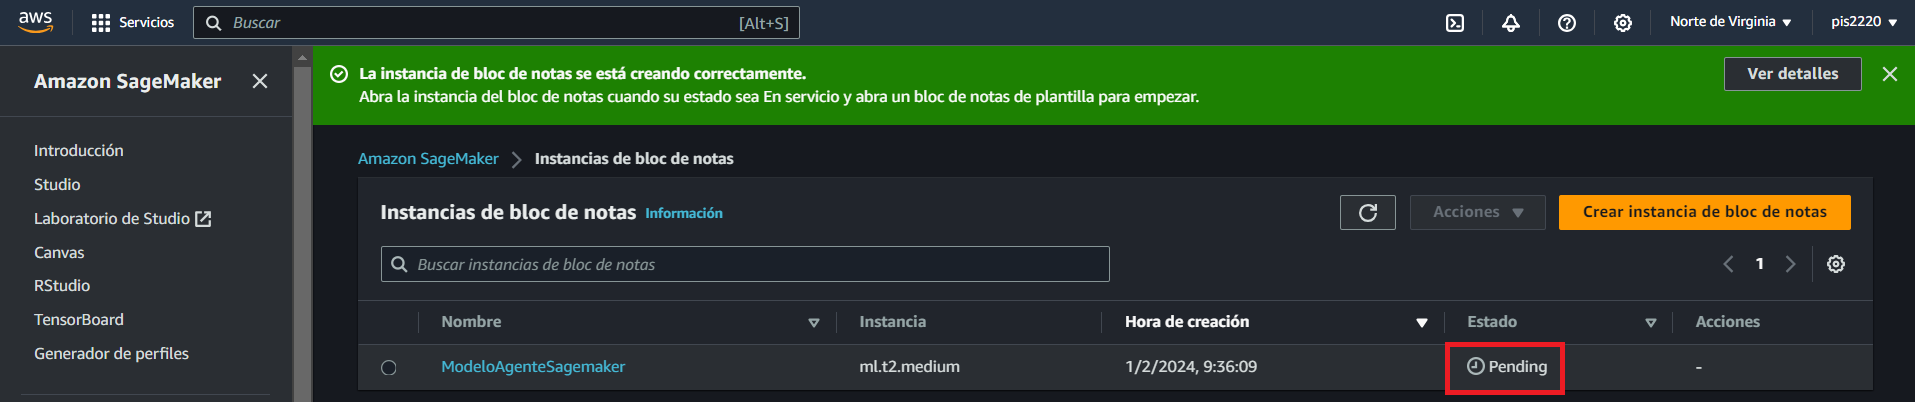
\includegraphics[width = 1\linewidth, height = 7.6cm]{Instancia_Creada_SageMaker.png}
		\caption{Instancia Creada SageMaker.}
		\label{Instancia_Creada_SageMaker}
	\end{figure}
	\begin{figure}[!h]
		\centering
		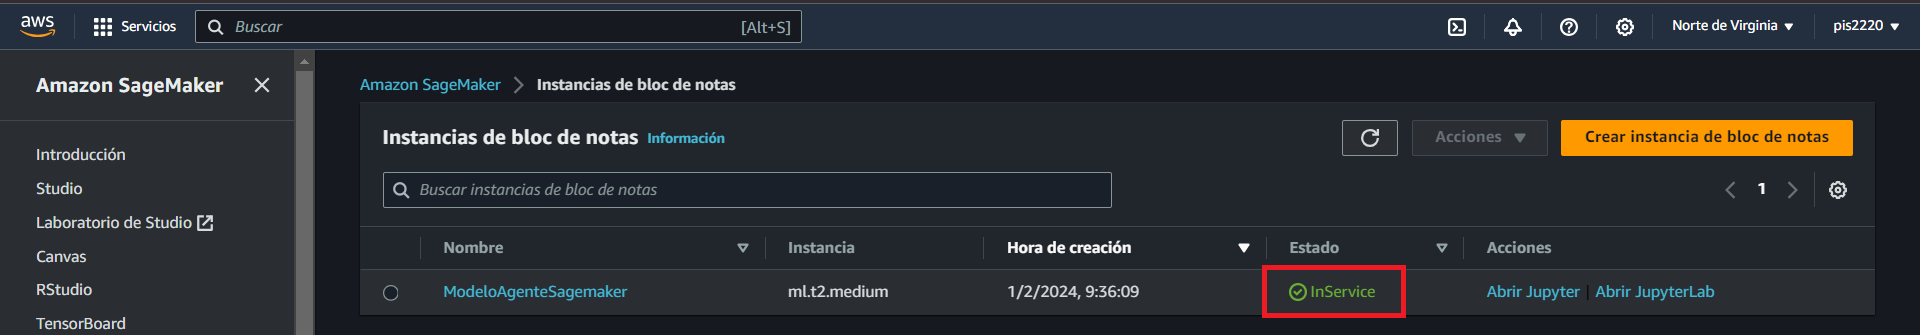
\includegraphics[width = 1\linewidth, height = 6.7cm]{Instancia_Creada_SageMaker_Online.png}
		\caption{Instancia Creada SageMaker en Servicio.}
		\label{Instancia_Creada_SageMaker_Online}
	\end{figure} \\
	\indent En este paso, se utiliza la instancia de cuaderno de Amazon SageMaker para pre-procesar los datos que se necesita para entrenar el modelo de machine learning y, a continuación, cargar los datos en Amazon S3. \\\newline
	\indent Después de que el estado de la instancia de cuaderno cambie a ``En Servicio'', seleccionar ``Abrir Jupyter'', como muestra la Figura \ref{SageMaker_Jupyter}.
	\begin{figure}[!h]
		\centering
		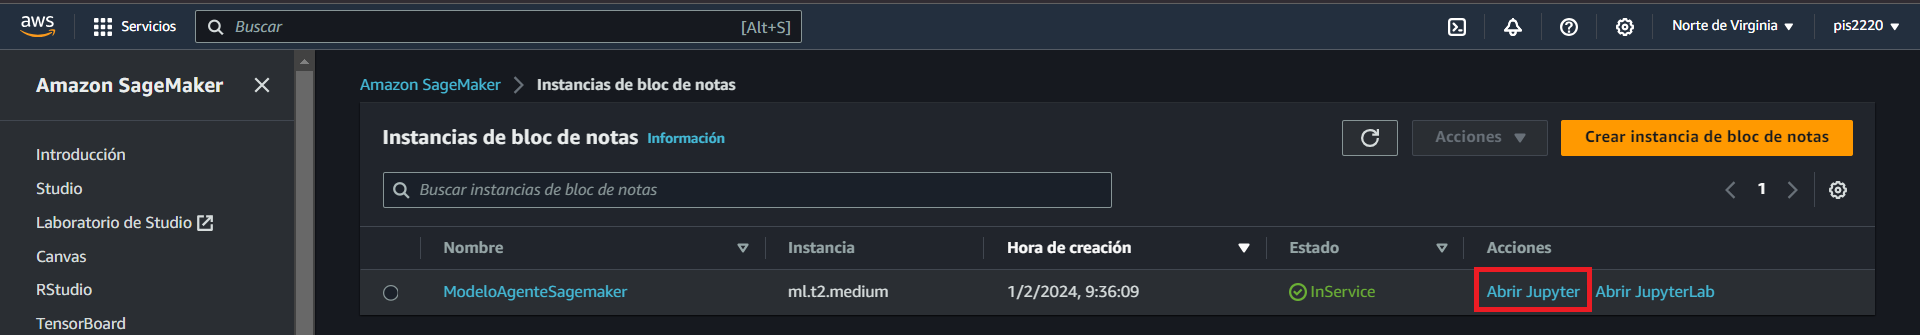
\includegraphics[width = 1\linewidth, height = 6.7cm]{SageMaker_Jupyter.png}
		\caption{Abrir Jupyter.}
		\label{SageMaker_Jupyter}
	\end{figure} \\
	\indent  JupyterLab es el último entorno de desarrollo interactivo basado en web para cuadernos, códigos y datos. Su interfaz flexible permite a los usuarios configurar y organizar flujos de trabajo en ciencia de datos, informática científica, periodismo computacional y aprendizaje automático. Un diseño modular invita a ampliaciones para ampliar y enriquecer la funcionalidad. \cite{Jupyter} \\\newline
	\indent En el entorno de Jupyter, seleccionar ``Cargar'' para poder subir el DataSet con el cual se va a trabajar, a seleccionar esta opción se abrirá un cuadro de dialogo que permitirá buscar en el equipo el DataSet y subirlo al entorno de Jupyter, ver Figura \ref{Jupyter_DataSet}. Una vez cargado se mostrara en la interfaz principal el DataSet, ver Figura \ref{Jupyter_DataSet_Cargado}.
	\begin{figure}[!h]
		\centering
		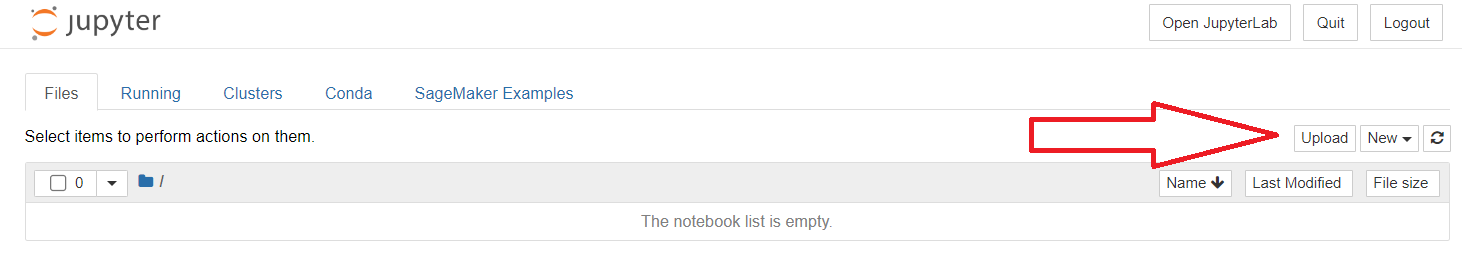
\includegraphics[width = 1\linewidth, height = 6.7cm]{Jupyter_DataSet.png}
		\caption{Jupyter DataSet.}
		\label{Jupyter_DataSet}
	\end{figure}
	\begin{figure}[!h]
		\centering
		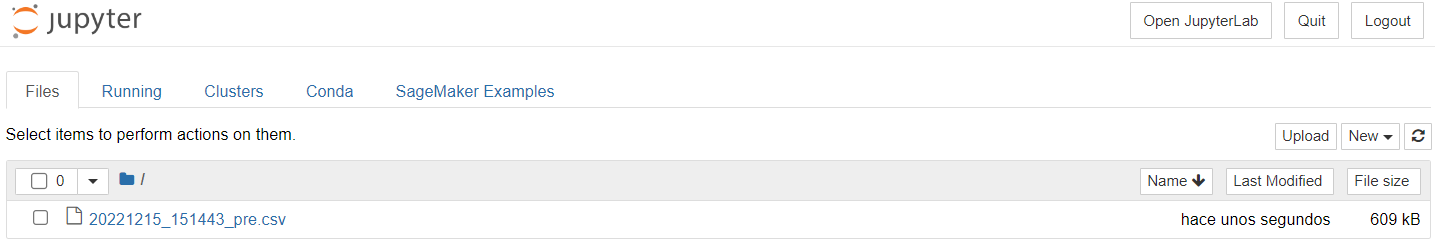
\includegraphics[width = 1\linewidth, height = 6.7cm]{Jupyter_DataSet_Cargado.png}
		\caption{Jupyter DataSet Cargado.}
		\label{Jupyter_DataSet_Cargado}
	\end{figure} \\
	\indent En el entorno de Jupyter, seleccionar ``Nuevo'' y a continuación, seleccionar ``conda\_python3'' como muestra la Figura \ref{Jupyter_Python}. Esto creara un nuevo NoteBook de Python, en el cual ya se puede comenzar a utilizar código de Python para crear el agente. En la sección de ``Archivo'', ``Guardar como'' se le puede cambiar el nombre al documento. En este caso se le pondrá el nombre de ``Modelo'', ver Figura \ref{Jupyter_Nombre}.
	\begin{figure}[!h]
		\centering
		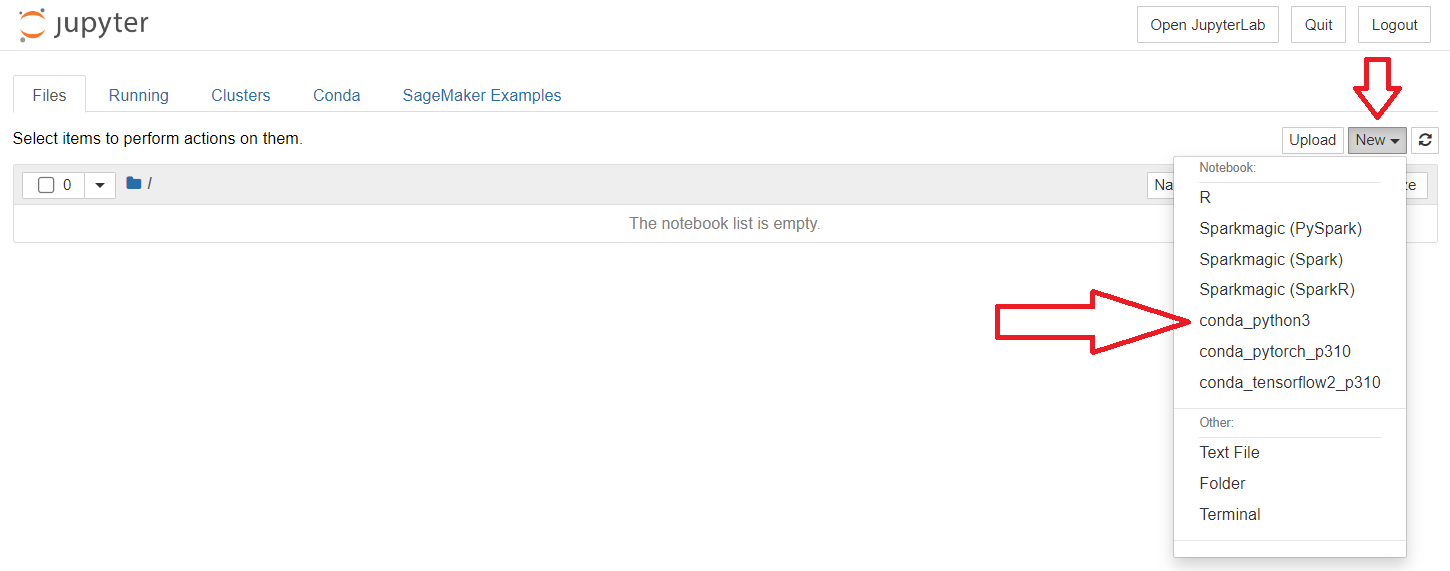
\includegraphics[width = 1\linewidth, height = 6.4cm]{Jupyter_Python.png}
		\caption{Entorno de Jupyter.}
		\label{Jupyter_Python}
	\end{figure}
	\begin{figure}[!h]
		\centering
		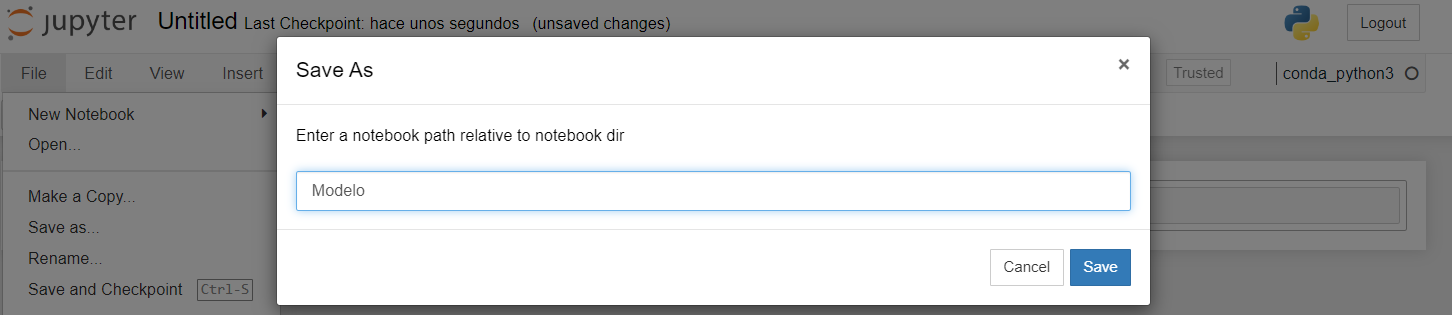
\includegraphics[width = 1\linewidth, height = 3.4cm]{Jupyter_Nombre.png}
		\caption{Cambio Nombre del Agente.}
		\label{Jupyter_Nombre}
	\end{figure} \\
	\indent Una vez subido el DataSet y configurado el nombre se puede comenzar a realizar código. El primer paso es crear un archivo con extensión ``py'', para ello seleccionar ``Nuevo'' y a continuación, seleccionar ``Archivo de Texto'' como muestra la Figura \ref{Jupyter_Nuevo_Py}
	\begin{figure}[!h]
		\centering
		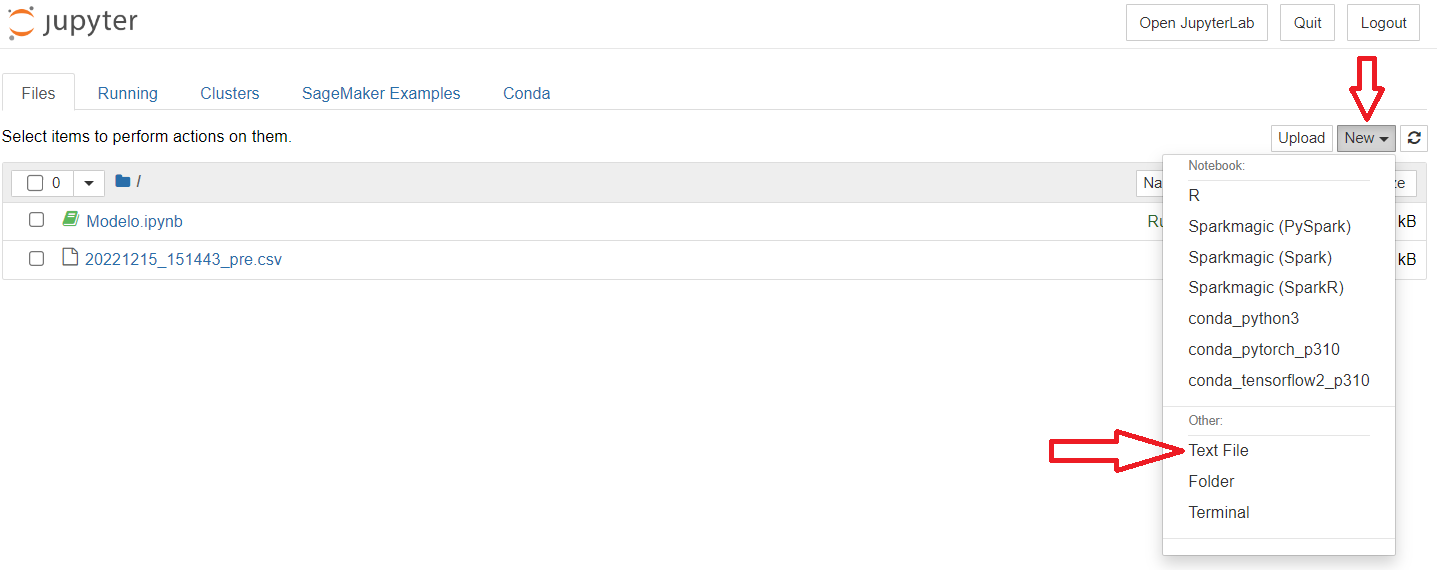
\includegraphics[width = 1\linewidth, height = 5.6cm]{Jupyter_Nuevo_Py.png}
		\caption{Nuevo Archivo de Texto.}
		\label{Jupyter_Nuevo_Py}
	\end{figure} \\
	\indent Al igual que en el caso anterior mostrado en la Figura \ref{Jupyter_Nombre}, se puede cambiar el nombre del archivo. En este caso se llamara al archivo ``Inference.py'', no olvidar poner la extensión ``.py'' en el nombre del documento. Una vez que se cambio el nombre se puede proceder a ingresar código en el interior del archivo, la Figura \ref{Inference_Codigo} muestra un segmento de código del archivo ``Inference.py''.
	\begin{figure}[!h]
		\centering
		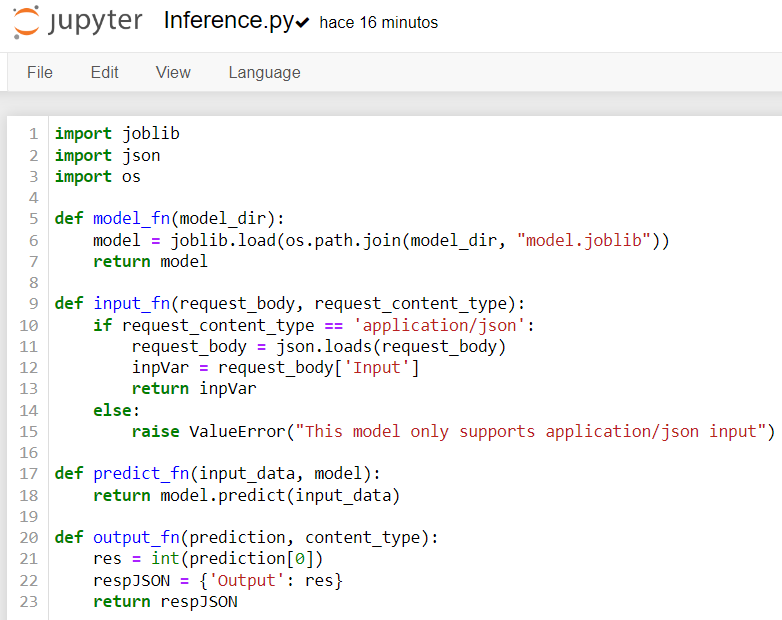
\includegraphics[width = 1\linewidth, height = 6.4cm]{Inference_Codigo.png}
		\caption{Código de Inference.py.}
		\label{Inference_Codigo}
	\end{figure} \\
	\indent En el archivo ``Modelo.ipynb'' creado anteriormente se programa el agente como tal, la Figura \ref{Modelo_Codigo} muestra una parte del código que se implemento.
	\begin{figure}[!h]
		\centering
		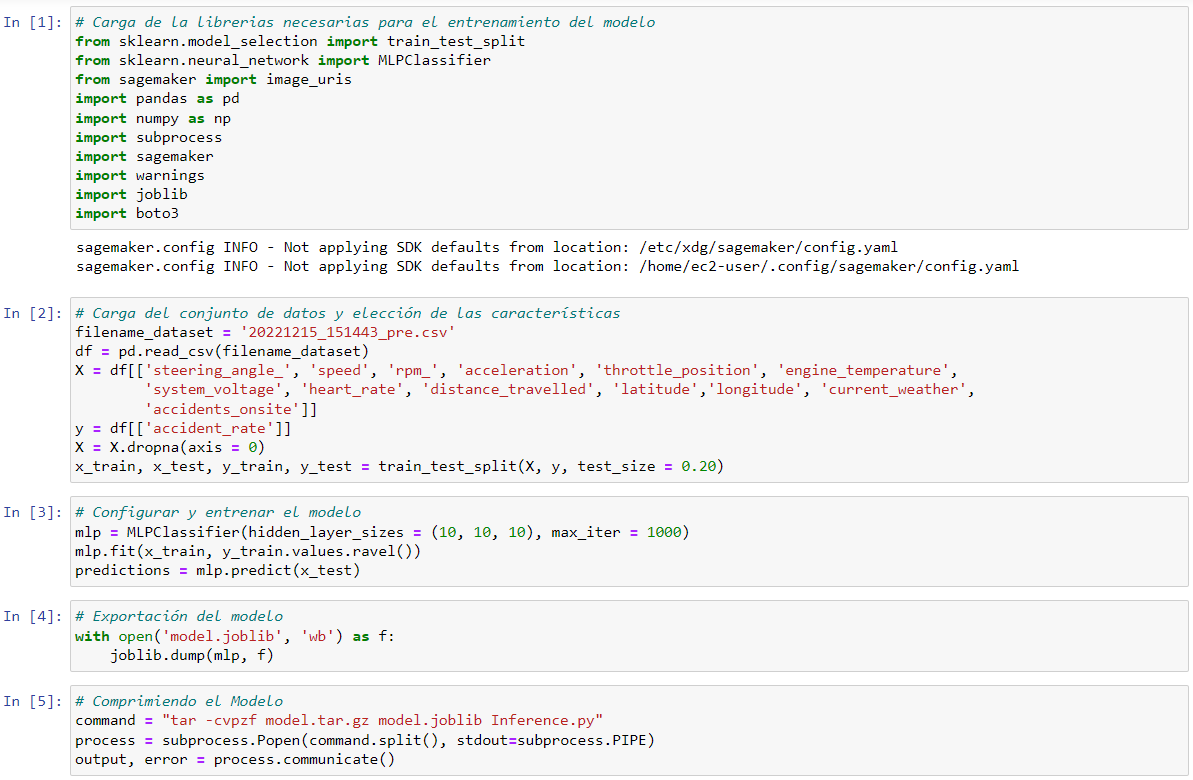
\includegraphics[width = 1\linewidth, height = 8.8cm]{Modelo_Codigo.png}
		\caption{Código de Modelo.ipynb.}
		\label{Modelo_Codigo}
	\end{figure} \\
	\indent Una vez que se ejecutaron todas la lineas de código en el NoteBook se puede observar varios resultados, los cuales se muestran a continuación:
	\begin{itemize}
		\item En JupyterLab se crearon varios archivos, ver Figura \ref{Jupyter_Archivos}.
		\item Se crea un nuevo Bucket de uso general, ver Figura \ref{S3_SageMaker_Bucket}.
		\item Se crea un nuevo Modelo de Inferencia, ver Figura \ref{SageMaker_Inferencia}.
		\item Se crea un nuevo punto de conexión, ver Figura \ref{SageMaker_Punto_Conexion}.
		\item Se crea un nuevo punto final, ver Figura \ref{SageMaker_EndPoint}. 
	\end{itemize}
	\begin{figure}[!h]
		\centering
		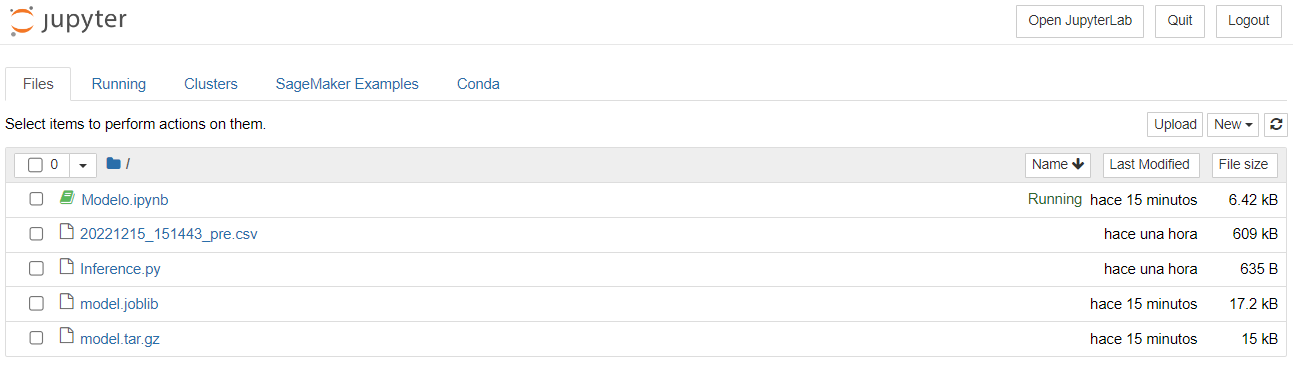
\includegraphics[width = 1\linewidth, height = 6.7cm]{Jupyter_Archivos.png}
		\caption{Jupyter Archivos.}
		\label{Jupyter_Archivos}
	\end{figure}
	\begin{figure}[!h]
		\centering
		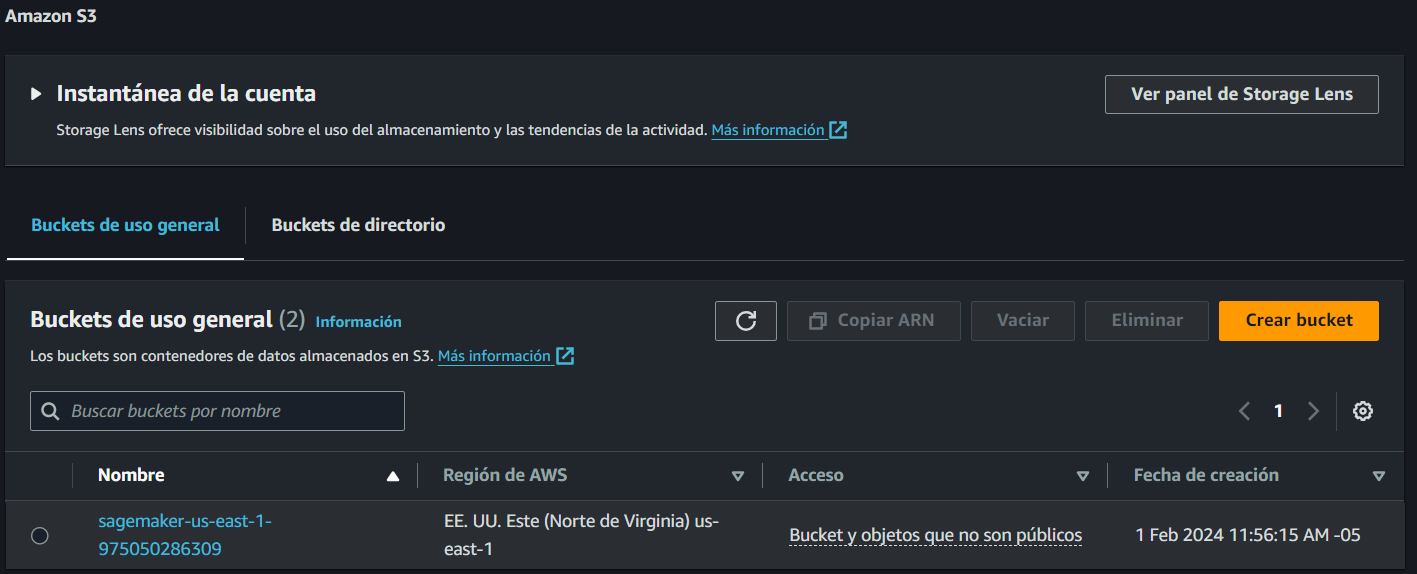
\includegraphics[width = 1\linewidth, height = 6.7cm]{S3_SageMaker_Bucket.png}
		\caption{S3 SageMaker Bucket.}
		\label{S3_SageMaker_Bucket}
	\end{figure}
	\begin{figure}[!h]
		\centering
		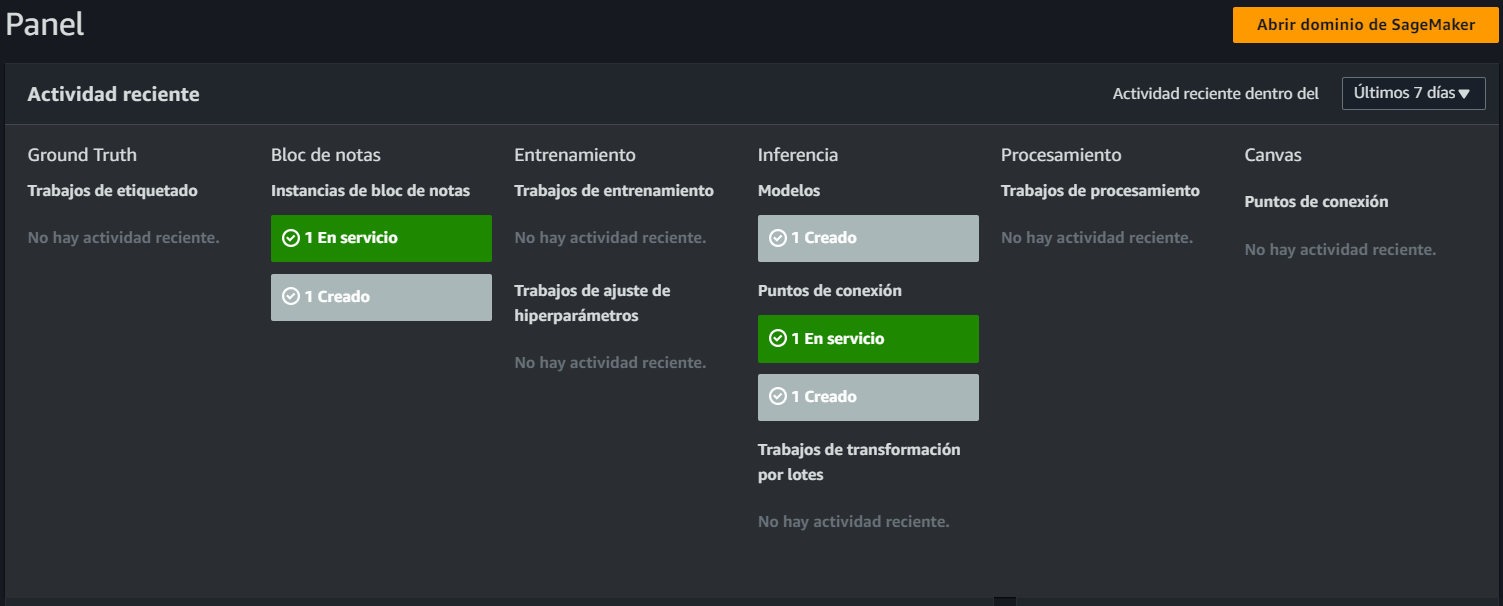
\includegraphics[width = 1\linewidth, height = 5.7cm]{SageMaker_Inferencia.png}
		\caption{SageMaker Inferencia.}
		\label{SageMaker_Inferencia}
	\end{figure}
	\begin{figure}[!h]
		\centering
		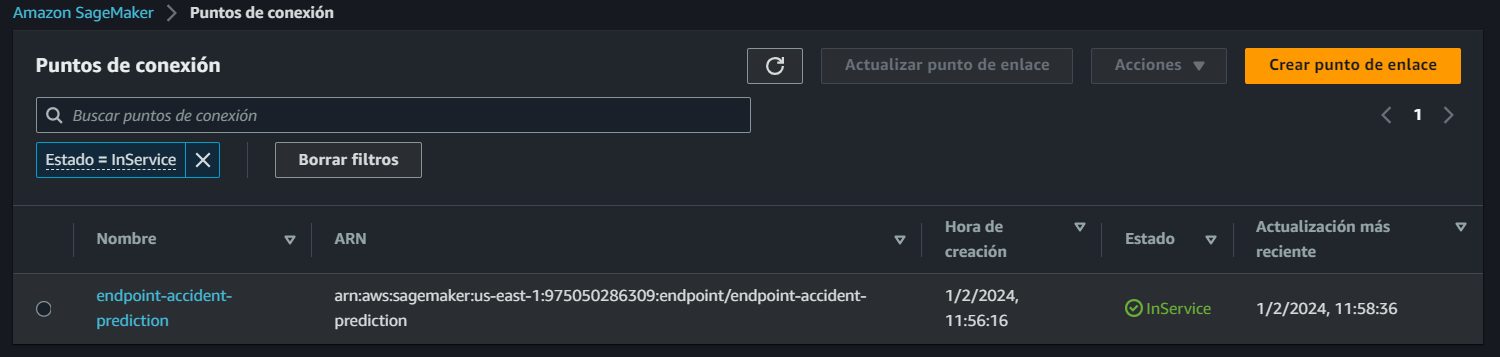
\includegraphics[width = 1\linewidth, height = 5.7cm]{SageMaker_Punto_Conexion.png}
		\caption{SageMaker Punto de Conexión.}
		\label{SageMaker_Punto_Conexion}
	\end{figure}
	\begin{figure}[!h]
		\centering
		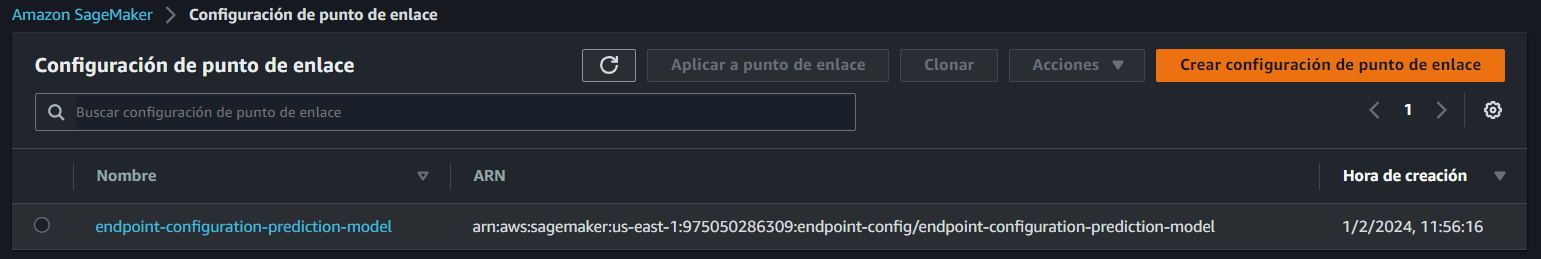
\includegraphics[width = 1\linewidth, height = 5.7cm]{SageMaker_EndPoint.png}
		\caption{SageMaker EndPoint.}
		\label{SageMaker_EndPoint}
	\end{figure}
	\indent \indent En el siguiente enlace se encuentra el código para generar y desplegar el modelo de predicción y la configuración para crear el punto final en el servicio Sagemaker:
	\begin{itemize}
		\item \textcolor{blue}{\url{https://github.com/laboratorioAI/PIS_20_02_AGENTES_IA/tree/main/Actualizacion_2024/Modelo}}
	\end{itemize}
	\subsubsection{Gestión de recursos informáticos - AWS Lambda}\label{AWS_Lambda}
	En este paso comprende la ``Gestión de recursos informáticos'' mediante AWS Lambda. AWS Lambda es un servicio informático sin servidor y basado en eventos que le permite ejecutar código para prácticamente cualquier tipo de aplicación o servicio backend sin necesidad de aprovisionar o administrar servidores \cite{Lambda}. En la Figura \ref{Funcionamiento_Lambda} se aprecia el funcionamiento de Lambda.
	\begin{figure}[!h]
		\centering
		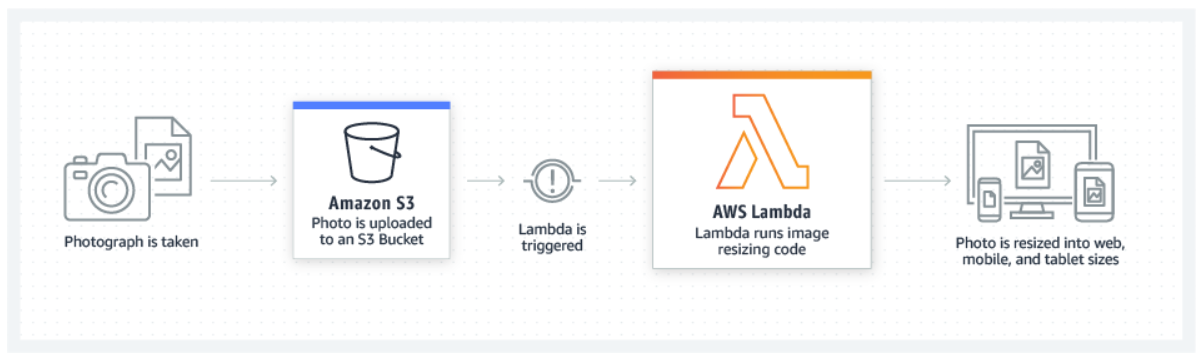
\includegraphics[width = 1\linewidth, height = 5.8cm]{Funcionamiento_Lambda.png}
		\caption{Funcionamiento de Lambda.}
		\label{Funcionamiento_Lambda}
	\end{figure} \\
	\indent Para incorporar este servicio es necesario ir a la consola de AWS y buscar el servicio de Lambda como muestra la Figura \ref{Servicio_Lambda}.
	\begin{figure}[!h]
		\centering
		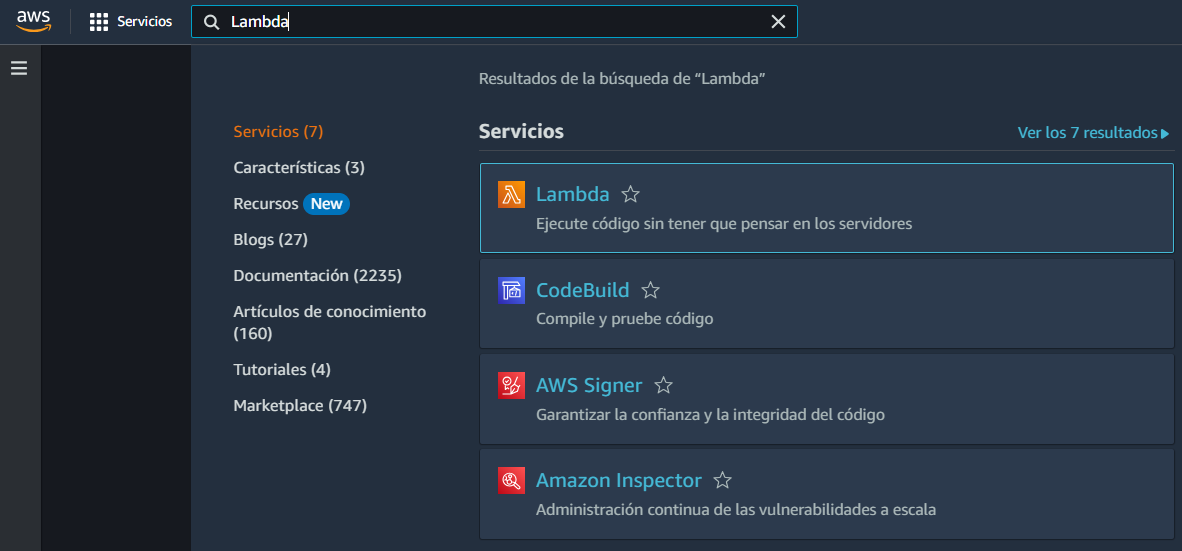
\includegraphics[width = 1\linewidth, height = 5.8cm]{Servicio_Lambda.png}
		\caption{Búsqueda Servicio Lambda.}
		\label{Servicio_Lambda}
	\end{figure} \\
	\indent Una vez dentro del panel de control de Lambda se debe crear una nueva función de Lambda dando ``Clic'' en el botón de ``Crear una función'', ver Figura \ref{Crear_Lambda}.
	\begin{figure}[!h]
		\centering
		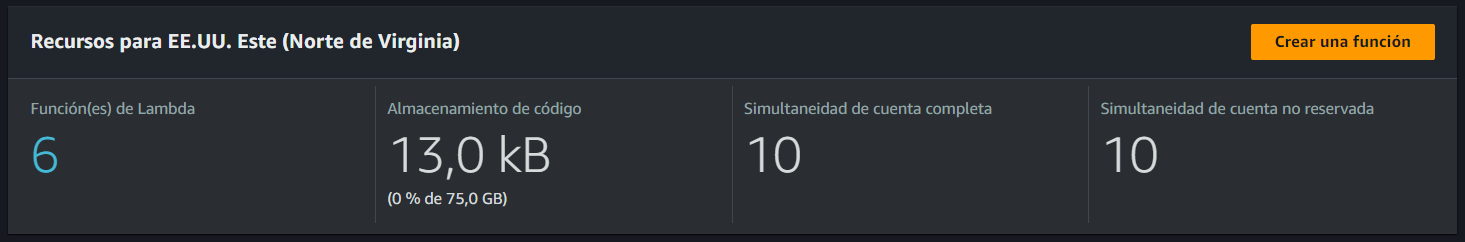
\includegraphics[width = 1\linewidth, height = 2.5cm]{Crear_Lambda.png}
		\caption{Crear Función Lambda.}
		\label{Crear_Lambda}
	\end{figure} \\
	\indent Una vez dentro de la consola de  ``Crear funciones Lambda'' es necesario configurar la función, ver Figura \ref{Configuracion_Lambda} de la siguiente manera: Tipo de función: Crear desde cero, El nombre de la función,Tiempo de ejecución: Python 3.12, Arquitectura: x86\_64, Rol de ejecución: Creación de un nuevo rol con permisos básicos de Lambda,Configuración avanzada: Habilitar URL de la función.
	\begin{figure}[!h]
		\centering
		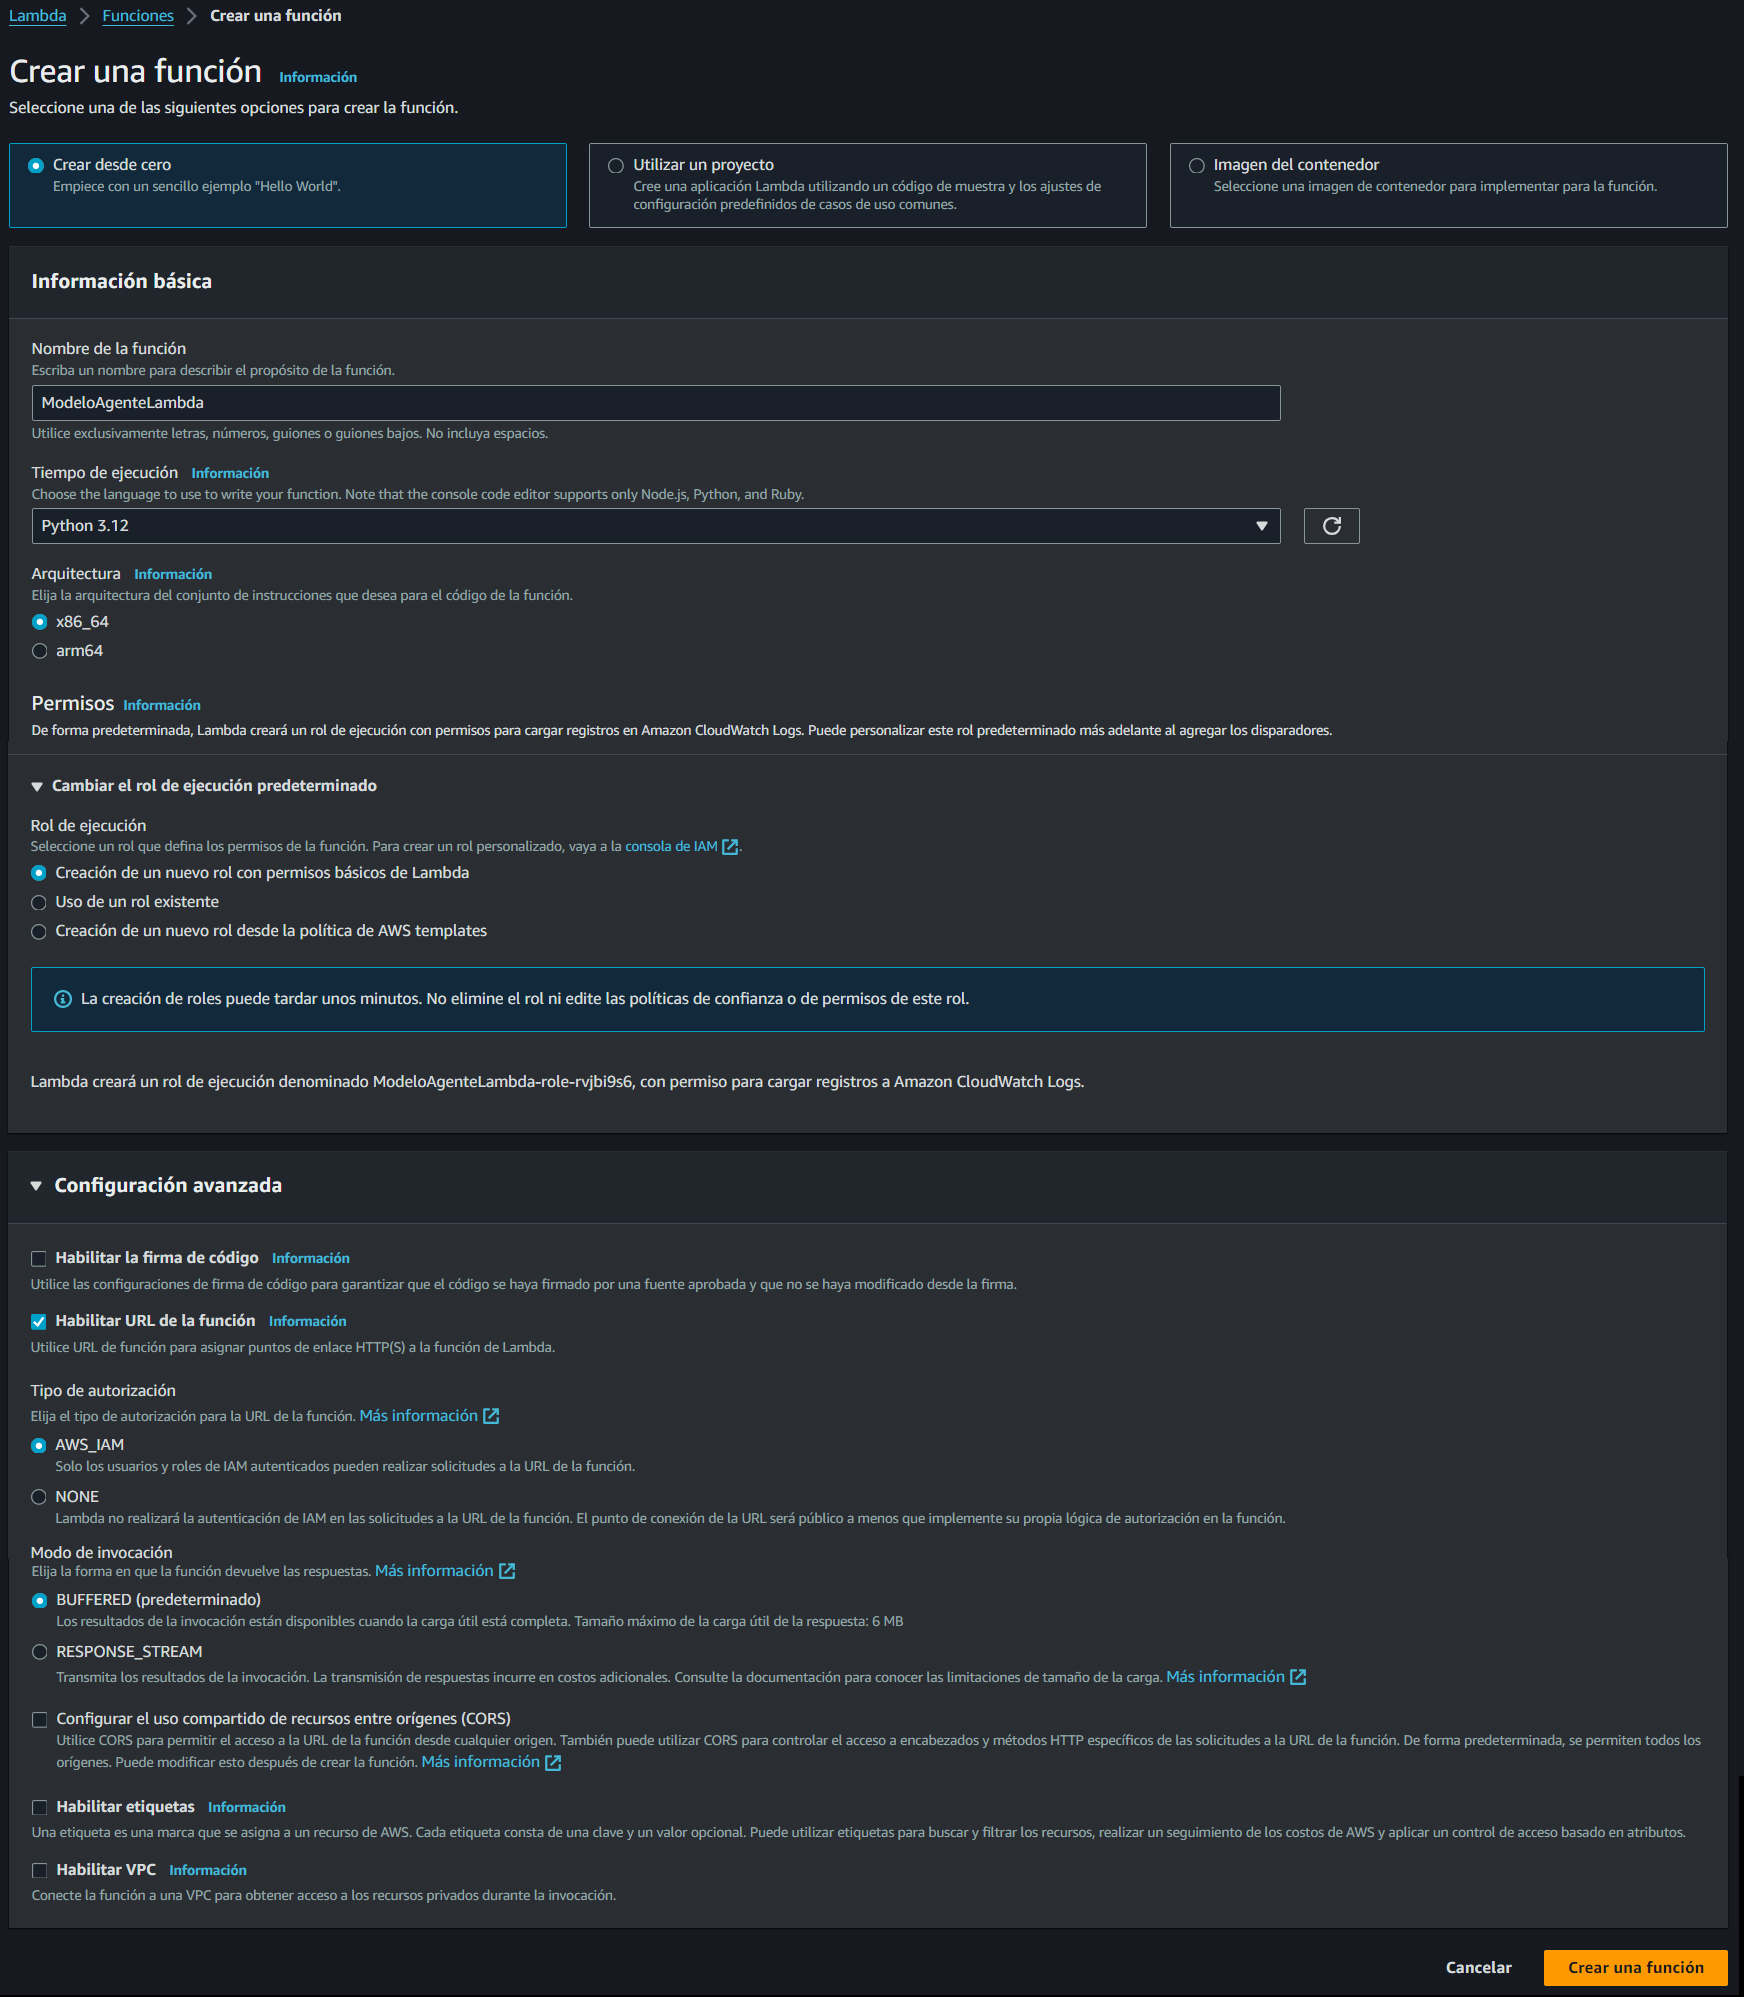
\includegraphics[width = 1\linewidth, height = 12.3cm]{Configuracion_Lambda.png}
		\caption{Configuración Lambda.}
		\label{Configuracion_Lambda}
	\end{figure} \\
	\indent Continuando con la configuración, en la pantalla mostrada en la Figura \ref{Modelo_Agente_Lambda}, se muestra el detalle de la función creada en Lambda. En este detalle se puede apreciar el diagrama dela función, el ARN de la función y la dirección URL de la función.
	\begin{figure}[!h]
		\centering
		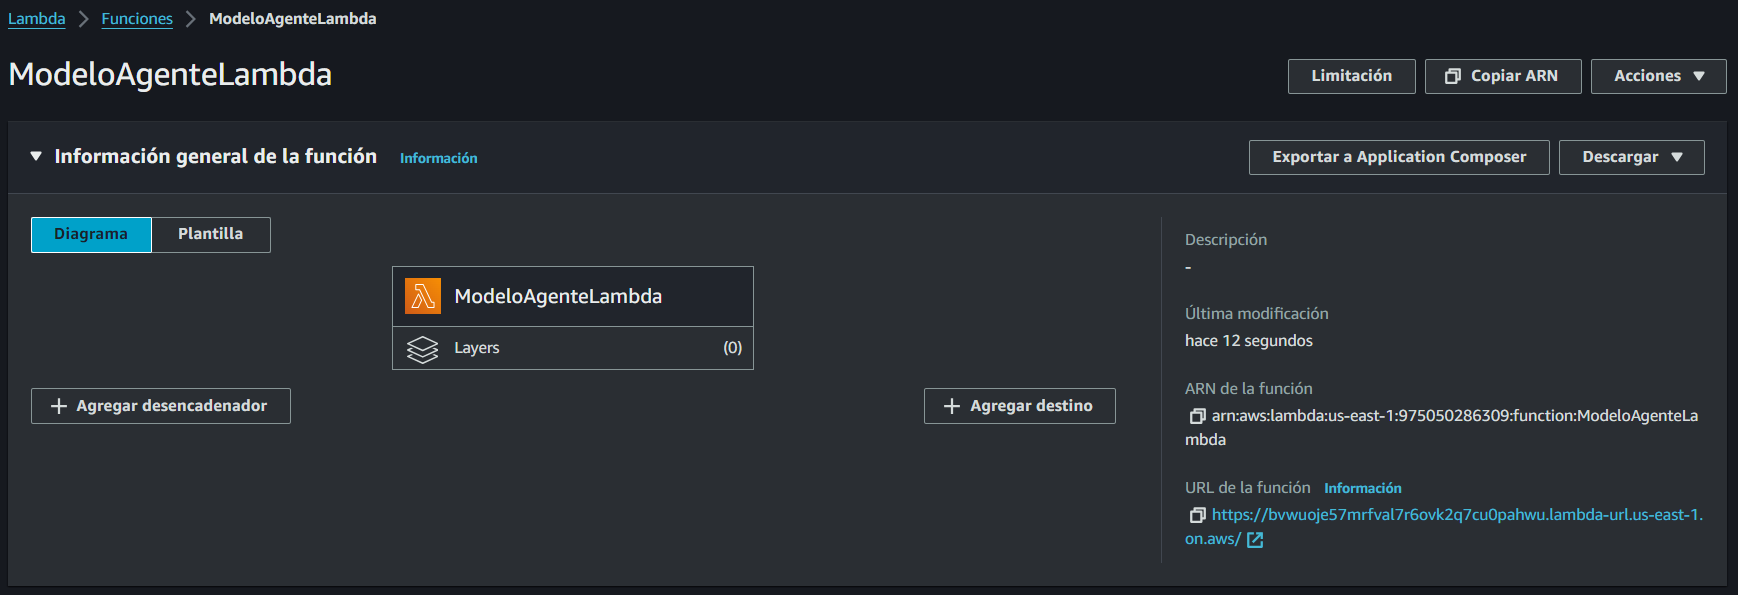
\includegraphics[width = 1\linewidth, height = 6cm]{Modelo_Agente_Lambda.png}
		\caption{Detalle Configuración Lambda.}
		\label{Modelo_Agente_Lambda}
	\end{figure} \\
	\indent Dentro de la misma pantalla en la parte baja, se puede encontrar la sección de ``Configuración'' y en ella la sección de ``Permisos'', donde se puede ver el ``Nombre del rol'' creado. Ver Figura \ref{Nombre_Rol_Lambda}. Si se hace ``Clic'' en el nombre del rol llevará a la consola de IAM y se podrá ver mas detalles sobre el rol.
	\begin{figure}[!h]
		\centering
		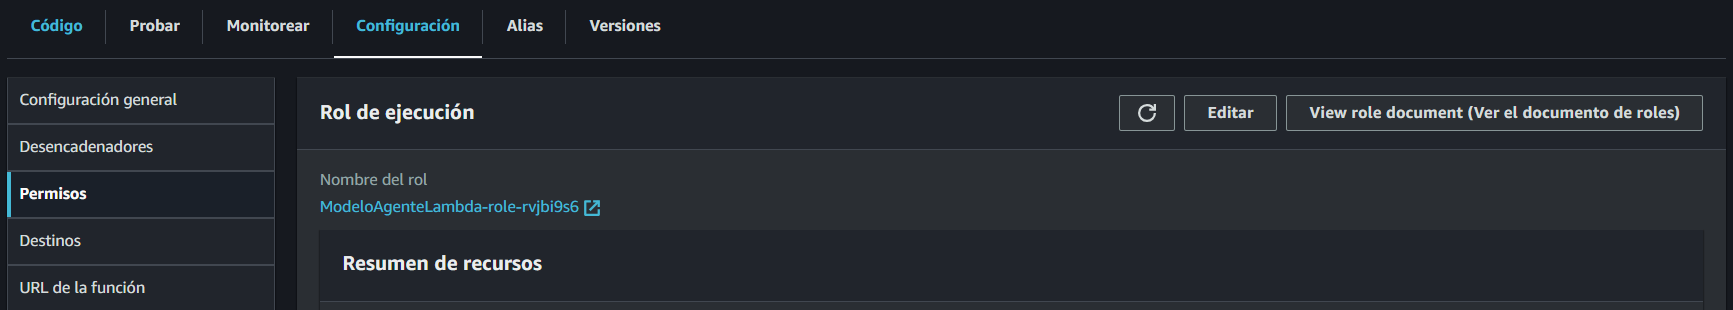
\includegraphics[width = 1\linewidth, height = 6.5cm]{Nombre_Rol_Lambda.png}
		\caption{Nombre de Rol Lambda.}
		\label{Nombre_Rol_Lambda}
	\end{figure} \\
	\indent En la nueva pantalla de debe crear una nueva política. Ya sea que haya creado una nueva función o se utilice una función existente, hay que asegúrese de incluir la siguiente política, que otorga a la función permiso para invocar un punto final del modelo, para ello se selecciona el nombre de la política como muestra la Figura \ref{Politica_Insertada}.
	\begin{figure}[!h]
		\centering
		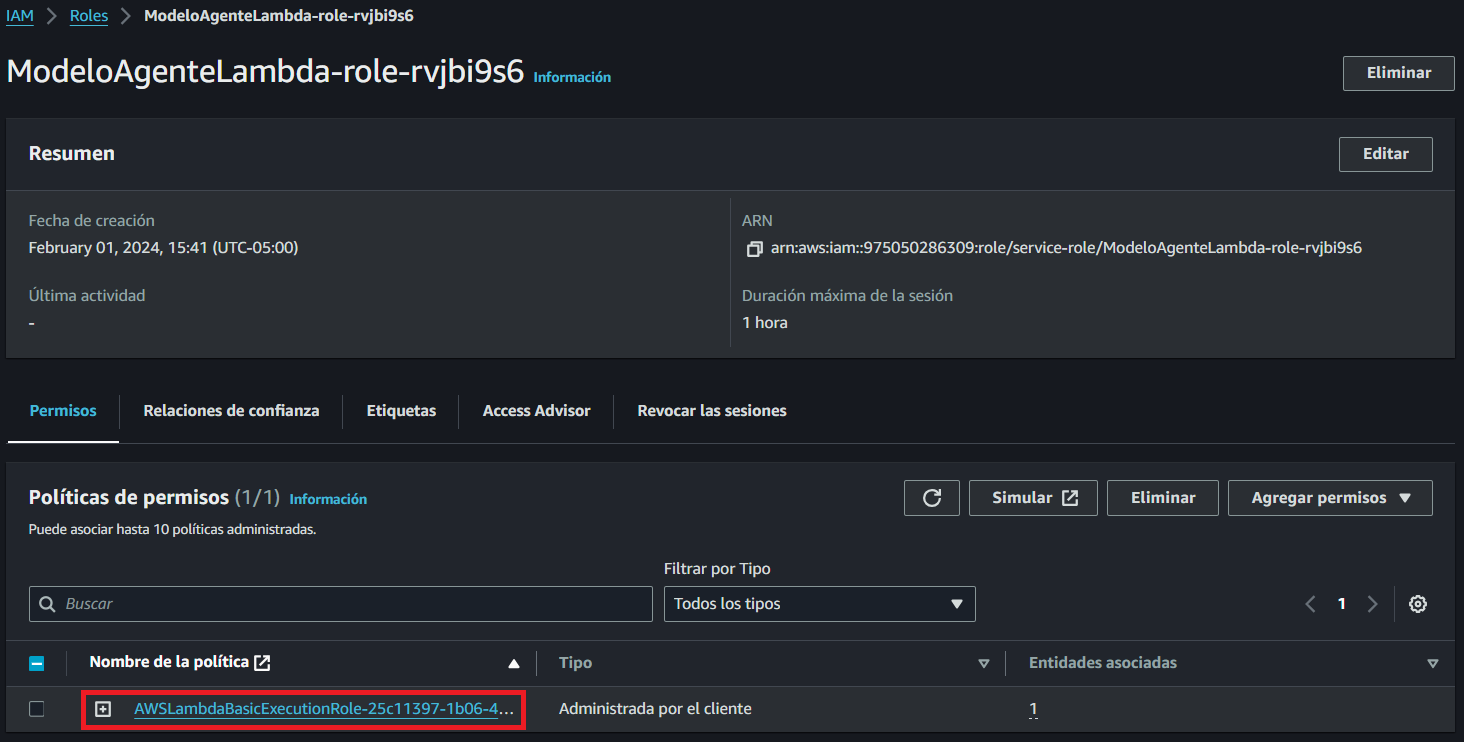
\includegraphics[width = 1\linewidth, height = 6.5cm]{Politica_Insertada.png}
		\caption{Crear política insertada.}
		\label{Politica_Insertada}
	\end{figure} \\
	\indent En la nueva pantalla de ``Permisos definidos en esta política'' se debe escoger la opción ``JSON'', ver Figura \ref{Politica_JSON}, y posteriormente seleccionar la opción ``Editar''y agregar la política manualmente como muestra la Figura \ref{Agregar_JSON}. Finalmente, se procede a finalizar con la creación de la política. Ver Figura \ref{Fin_Politica_Lambda}.
	\begin{figure}[!h]
		\centering
		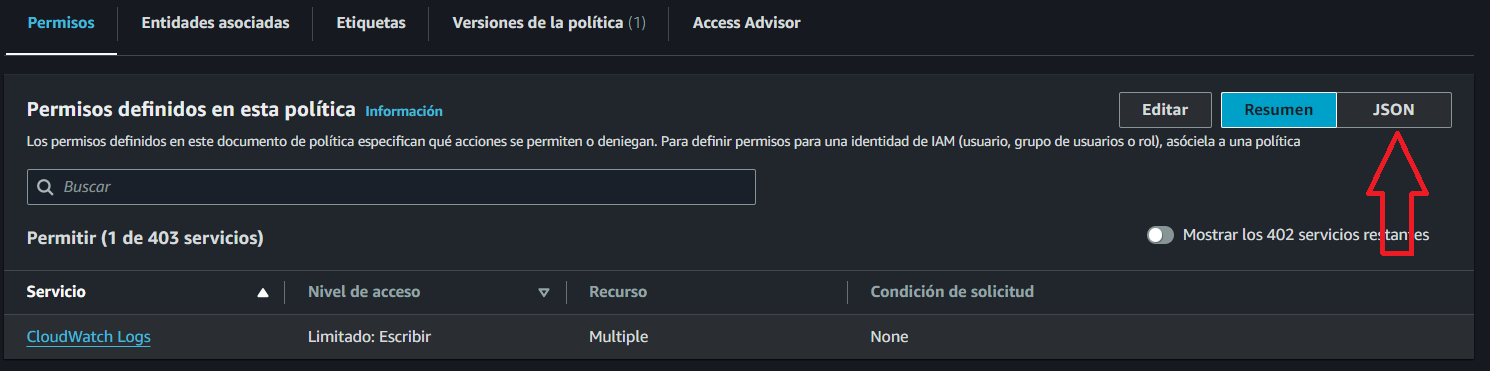
\includegraphics[width = 1\linewidth, height = 10.1cm]{Politica_JSON.png}
		\caption{Selección JSON.}
		\label{Politica_JSON}
	\end{figure}
	\begin{figure}[!h]
		\centering
		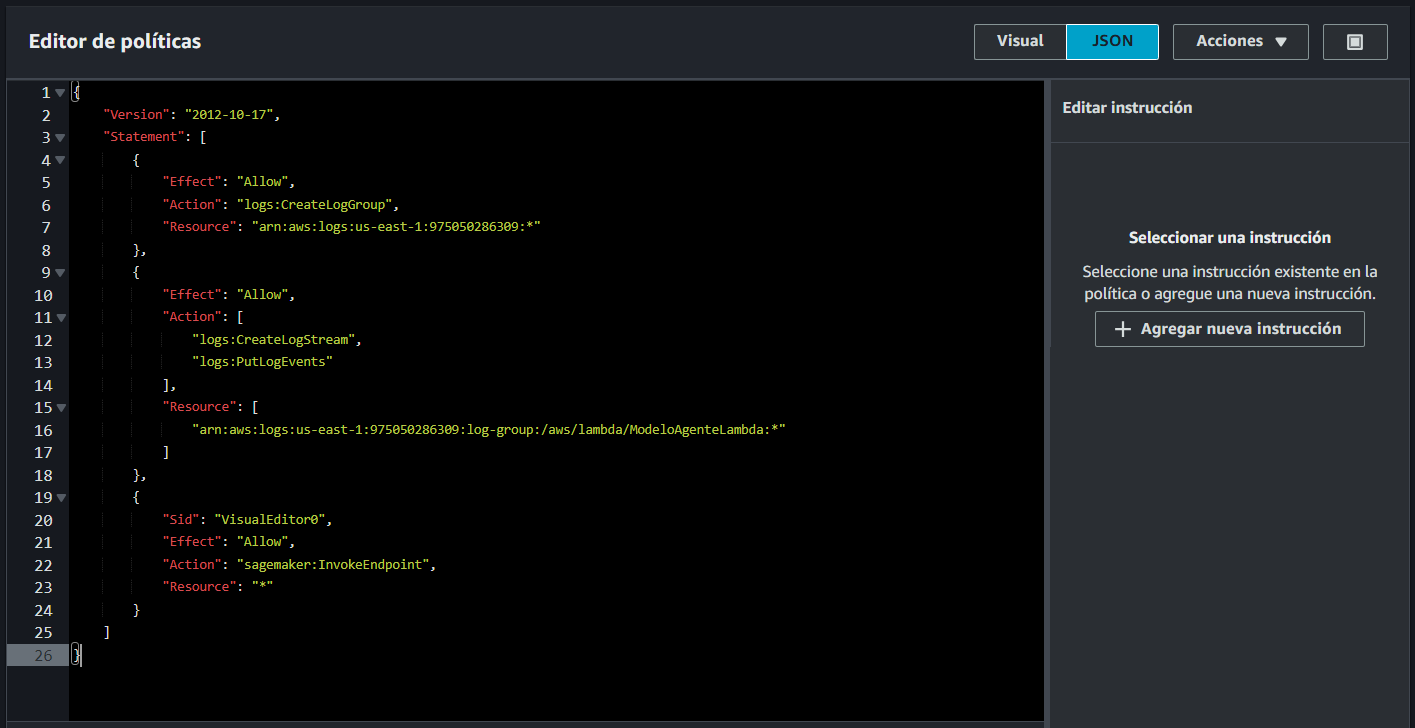
\includegraphics[width = 1\linewidth, height = 6cm]{Agregar_JSON.png}
		\caption{Política insertada JSON.}
		\label{Agregar_JSON}
	\end{figure}
	\begin{figure}[!h]
		\centering
		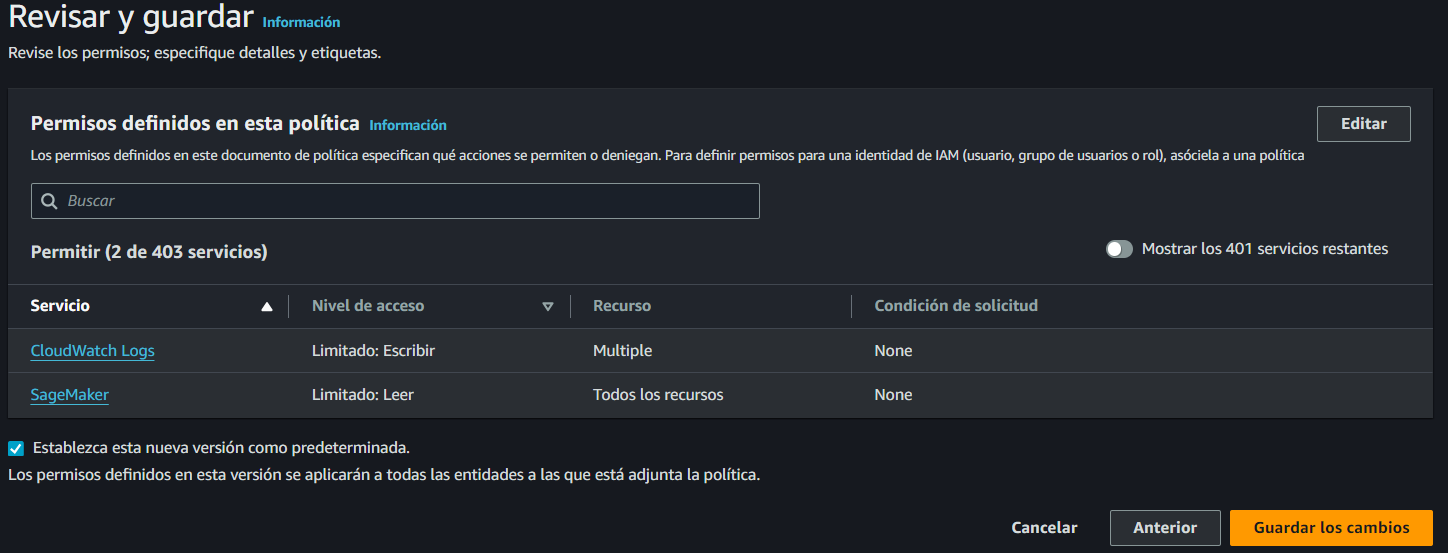
\includegraphics[width = 1\linewidth, height = 4.1cm]{Fin_Politica_Lambda.png}
		\caption{Creación total política insertada.}
		\label{Fin_Politica_Lambda}
	\end{figure} \\
	\indent Tras finalizar se puede apreciar en la pantalla principal que la nueva política ha sido creada con éxito, ver Figura \ref{Resumen_Politica_Lambda}. esta política se creo automáticamente con el nombre de ``SageMaker''.
	\begin{figure}[!h]
		\centering
		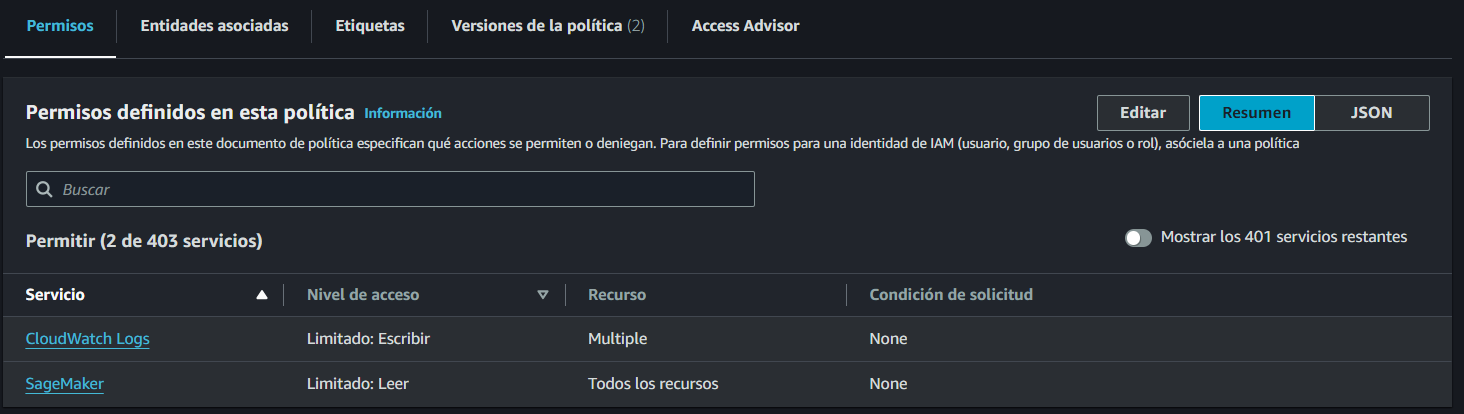
\includegraphics[width = 1\linewidth, height = 4.1cm]{Resumen_Politica_Lambda.png}
		\caption{Resumen Políticas Lambda.}
		\label{Resumen_Politica_Lambda}
	\end{figure} \\
	\indent Regresando al panel de control de Lambda se procede a programas el código fuente de la función Lambda, en la Figura \ref{Codigo_Fuente_Lambda} se muestra el código fuente antes de desplegar la función Lambda.
	\begin{figure}[!h]
		\centering
		\includegraphics[width = 1\linewidth, height = 4.3cm]{Codigo_Fuente_Lambda.png}
		\caption{Código Fuente Lambda.}
		\label{Codigo_Fuente_Lambda}
	\end{figure} \\
	\indent Luego de ingresar el código fuente, en la misma pantalla se ingresa en la opción ``Configuración'' y luego en ``Variables de entorno'' seleccionamos la opción ``Editar'', ver Figura \ref{Variables_Entorno}. Esto redirigirá al usuario a una nueva consola donde deberá configurar las Variables de entorno.
	\begin{figure}[!h]
		\centering
		\includegraphics[width = 1\linewidth, height = 4.3cm]{Variables_Entorno.png}
		\caption{Variables de Entorno.}
		\label{Variables_Entorno}
	\end{figure} \\
	\indent En la pantalla de configuración de variables se debe escoger la opción ``Agregar variable de entorno'' y agregar la ``Clave'' y el ``Valor'' como muestra la Figura \ref{Variable_EndPoint}. En el campo de Clave se debe poner la siguiente información: ``ENDPOINT\_NAME'', mientras que en el campos de valor se debe poner la información que se presenta en la Figura \ref{SageMaker_Punto_Conexion}.
	\begin{figure}[!h]
		\centering
		\includegraphics[width = 1\linewidth, height = 4.3cm]{Variable_EndPoint.png}
		\caption{Configuración de Variable de Entorno.}
		\label{Variable_EndPoint}
	\end{figure} \\
	\indent Tras guardar la configuración realizada se puede observar que en el panel de funciones de Lambda en la sección Configuración y Variables de entorno se a creado con éxito el ``EndPoint'' de Lambda, ver Figura \ref{EndPoint_Creado}.
	\begin{figure}[!h]
		\centering
		\includegraphics[width = 1\linewidth, height = 5cm]{EndPoint_Creado.png}
		\caption{EndPoint Creado.}
		\label{EndPoint_Creado}
	\end{figure} \\
	\indent Finalmente, en la misma pantalla se regresa a la sección de ``Código'' y se presiona el botón de ``Deploy'' para desplegar la función Lambda como muestra la Figura \ref{Deploy_Lambda}.
	\begin{figure}[!h]
		\centering
		\includegraphics[width = 1\linewidth, height = 5cm]{Deploy_Lambda.png}
		\caption{Deploy Función Lambda.}
		\label{Deploy_Lambda}
	\end{figure} \\
	\indent En el siguiente enlace se encuentra el código de implementación de la función Lambda:
	\begin{itemize}
		\item \textcolor{blue}{\url{https://github.com/laboratorioAI/PIS_20_02_AGENTES_IA/tree/main/Actualizacion_2024/Lambda}}
	\end{itemize}
	\subsection{API Management - AWS API Gateway}\label{AWS_Gateway_API}
	El ultimo paso de esta etapa es crear el API Gateway que desencadena el evento que invoca la función Lambda simplemente pasando los datos de prueba a través de un evento. Amazon API Gateway es un servicio completamente administrado que facilita a los desarrolladores la creación, la publicación, el mantenimiento, el monitoreo y la protección de API a cualquier escala. Las API actúan como la "puerta de entrada" para que las aplicaciones accedan a los datos, la lógica empresarial o la funcionalidad de sus servicios de backend. Con API Gateway, puede crear API RESTful y API WebSocket que permiten aplicaciones de comunicación bidireccional en tiempo real. API Gateway admite cargas de trabajo en contenedores y sin servidor, así como aplicaciones web \cite{Gateway}. En la Figura \ref{Funcionamiento_Gateway} se aprecia el funcionamiento de API Gateway.
	\begin{figure}[!h]
		\centering
		\includegraphics[width = 1\linewidth, height = 4cm]{Funcionamiento_Gateway.png}
		\caption{Funcionamiento de API Gateway.}
		\label{Funcionamiento_Gateway}
	\end{figure} \\
	\indent Para crear una ``API REST'' en el panel de control de AWS se debe buscar el servicio de ``API Gateway'' como muestra la Figura \ref{Servicio_Gateway}.
	\begin{figure}[!h]
		\centering
		\includegraphics[width = 1\linewidth, height = 4cm]{Servicio_Gateway.png}
		\caption{Búsqueda Servicio API Gateway.}
		\label{Servicio_Gateway}
	\end{figure} \\
	\indent Tras ingresar al panel de control de ``API Gateway'' se debe escoger el tipo de API que se va a utilizar, para el desarrollo de este trabajo se escoge la opción de ``API REST'', como muestra la Figura \ref{Seleccion_API_REST} y en esta se escoge la opción ``Crear''. 
	\begin{figure}[!h]
		\centering
		\includegraphics[width = 1\linewidth, height = 3.9cm]{Seleccion_API_REST.png}
		\caption{Selección API REST.}
		\label{Seleccion_API_REST}
	\end{figure} \\
	\indent Tras elegir la opción de ``Crear'' se redirigirá al usuario a una nueva pantalla, donde se debe configura varios parámetros como: Tipo API: se escoge ``Nueva API'', Nombre de API, Descripción: es una descripción ligera de la API, es opcional y Tipo de punto de conexión de la API: ``Regional''. \\\newline
	\indent Al finalizar con la configuración de los parámetros, ver Figura \ref{Crear_API_Gateway}, se presiona el botón de ``Crear API'' lo cual redirigirá al marco de trabajo de la API donde se puede apreciar que esta se ha creado con éxito.
	\begin{figure}[!h]
		\centering
		\includegraphics[width = 1\linewidth, height = 4.5cm]{Crear_API_Gateway.png}
		\caption{Crear API Gateway.}
		\label{Crear_API_Gateway}
	\end{figure} \\
	\indent Una vez creada el API, en el menú ``Recurso'', se elije ``Crear recurso'', ver Figura \ref{Crear_Recurso_API}. Esto abrirá una interfaz donde se configurara los ``Detalles del recurso''. En la Figura \ref{Recursos_Predictor_Accidentes} se muestra la configuración del recurso creado.
	\begin{figure}[!h]
		\centering
		\includegraphics[width = 1\linewidth, height = 3.7cm]{Crear_Recurso_API.png}
		\caption{Crear Recurso API.}
		\label{Crear_Recurso_API}
	\end{figure}
	\begin{figure}[!h]
		\centering
		\includegraphics[width = 1\linewidth, height = 3.7cm]{Recursos_Predictor_Accidentes.png}
		\caption{Detalles del Recurso.}
		\label{Recursos_Predictor_Accidentes}
	\end{figure} \\
	\indent Una vez creado el recurso, en el menú ``Métodos'', se elije ``Crear método'' para crear un método POST, ver Figura \ref{Crear_Metodo_POST}. Esto abrirá una interfaz donde se configurara los ``Detalles del método''. En estos detalles se configura el ``Tipo de integración'': Función Lambda, la ``Región'' y el ``ARN'' de la función Lambda, el ARN se encuentra detallado en la Figura \ref{Politica_Insertada}, y el tiempo de espera predeterminado que se establece es de 29 segundos por defecto. Ver Figura \ref{Detalles_Metodo_POST}.
	\begin{figure}[!h]
		\centering
		\includegraphics[width = 1\linewidth, height = 5cm]{Crear_Metodo_POST.png}
		\caption{Crear Método POST.}
		\label{Crear_Metodo_POST}
	\end{figure}
	\begin{figure}[!h]
		\centering
		\includegraphics[width = 1\linewidth, height = 10.6cm]{Detalles_Metodo_POST.png}
		\caption{Detalles Método POST.}
		\label{Detalles_Metodo_POST}
	\end{figure} \\
	\indent Al finalizar solo basta con desplegar la API, para ello se presiona el botón ``Implementar API'' como muestra la Figura \ref{Deploy_API_Gateway}. Esto llevara a una interfaz donde se detalla la información final sobre la API como: Etapa, Nombre de la Etapa y Descripción de la implementación. Ver Figura \ref{Detalles_Deploy_API}. Este paso le proporciona la URL de invocación. Ver Figura \ref{API_Implementada_Completa}.
	\begin{figure}[!h]
		\centering
		\includegraphics[width = 1\linewidth, height = 4.8cm]{Deploy_API_Gateway.png}
		\caption{Deploy API Gateway.}
		\label{Deploy_API_Gateway}
	\end{figure}
	\begin{figure}[!h]
		\centering
		\includegraphics[width = 1\linewidth, height = 4.8cm]{Detalles_Deploy_API.png}
		\caption{Detalles Deploy API Gateway.}
		\label{Detalles_Deploy_API}
	\end{figure}
	\begin{figure}[!h]
		\centering
		\includegraphics[width = 1\linewidth, height = 4.8cm]{API_Implementada_Completa.png}
		\caption{API Implementada Completamente.}
		\label{API_Implementada_Completa}
	\end{figure}
	\subsection{Pruebas de Funcionamiento POST/REST}
	Tras realizar todas las implementaciones, solo falta realizar las pruebas de funcionamiento. Para realizar las pruebas de funcionamiento se hará uso del entorno JupyterLab. En la Figura \ref{Codigo_Cliente_JupyterLab} se muestra el código implementado en Python, mientras que la Figura \ref{Comando_Ejecucion} se muestras los resultados de las consultas POST/REST realizadas hacia el agente.
	\begin{figure}[!h]
		\centering
		\includegraphics[width = 1\linewidth, height = 6.7cm]{Codigo_Cliente_JupyterLab.png}
		\caption{Código Cliente JupyterLab.}
		\label{Codigo_Cliente_JupyterLab}
	\end{figure}
	\begin{figure}[!h]
		\centering
		\includegraphics[width = 1\linewidth, height = 6.7cm]{Comando_Ejecucion.png}
		\caption{Resultados Consulta POST/REST.}
		\label{Comando_Ejecucion}
	\end{figure} \\
	\indent En el siguiente enlace se encuentra el código de implementación para las pruebas de funcionamiento:
	\begin{itemize}
		\item \textcolor{blue}{\url{https://github.com/laboratorioAI/PIS_20_02_AGENTES_IA/tree/main/Actualizacion_2024/Cliente}}
	\end{itemize}
	
	\section{Implementación APP Móvil - Android Studio}
	La implementación de una aplicación móvil en Android Studio implica un proceso completo de desarrollo que abarca desde la concepción de la idea hasta la entrega final del producto. Android Studio, siendo el entorno de desarrollo oficial respaldado por Google, juega un papel central en este proceso, proporcionando herramientas poderosas y funcionalidades que facilitan la creación de aplicaciones Android robustas y efectivas \cite{Android}. \\\newline
	\indent El primer paso en la implementación de una aplicación es la configuración del entorno de desarrollo. Esto implica descargar e instalar Android Studio, así como configurar el entorno con los componentes necesarios, como los paquetes de desarrollo de software (SDK) y las herramientas específicas de Android. Este paso es crucial para garantizar que el desarrollador tenga acceso a las bibliotecas y recursos necesarios para construir y probar la aplicación de manera efectiva.
	\subsection{Aplicaciones Web y Móviles - AWS Amplify}
	AWS Amplify Hosting es un servicio de alojamiento y CI/CD completamente administrado para aplicaciones estáticas, rápidas, seguras, fiables, renderizadas del lado del servidor y que escalan con su empresa. Es compatible con marcos web modernos como React, Angular, Vue, Next.js, Gatsby, Hugo, Jekyll, entre otros \cite{Amplify}. En la Figura \ref{Funcionamiento_Amplify} se aprecia el funcionamiento de AWS Amplify.
	\begin{figure}[!h]
		\centering
		\includegraphics[width = 1\linewidth, height = 6.2cm]{Funcionamiento_Amplify.png}
		\caption{Funcionamiento de AWS Amplify.}
		\label{Funcionamiento_Amplify}
	\end{figure} \\
	\indent El primer paso es instalar Node.js en el computador de trabajo desde la siguiente URL: \textcolor{blue}{\url{https://nodejs.org/en/download/}}, de existir problemas se puede encontrar documentación en la siguiente pagina \textcolor{blue}{\url{https://docs.npmjs.com/downloading-and-installing-node-js-and-npm}}. Ver Figura \ref{Repositorio_Nodes}. \\\newline
	\indent El siguiente paso es el instalar la consola de ``Amplify'' mediante el comando de la Figura \ref{Comando_Amplify}, para ello se debe abrir una terminal en modo administrador y ejecutar el comando.
	\begin{figure}[!h]
		\centering
		\includegraphics[width = 1\linewidth, height = 4cm]{Repositorio_Nodes.png}
		\caption{Repositorio Nodes.}
		\label{Repositorio_Nodes}
	\end{figure} \\
	\indent De preferencia y por seguridad se debe abrir dentro del entorno de desarrollo de ``Android Studio'' ejecutándolo como ``Administrador''. Ver Figura \ref{Comando_Amplify}.
	\begin{figure}[!h]
		\centering
		\includegraphics[width = 1\linewidth, height = 3.5cm]{Comando_Amplify.png}
		\caption{Comando de Instalación de Amplify.}
		\label{Comando_Amplify}
	\end{figure} \\
	\indent Continuando, se debe abrir Android Studio en modo Administrador. Posteriormente, en el proyecto en el cual se está trabajando se debe abrir la consola de comando. Ver Figura \ref{Consola_Android}. Para ver como crear un nuevo proyecto ver el apartado \ref{Nuevo_Android}.
	\begin{figure}[!h]
		\centering
		\includegraphics[width = 1\linewidth, height = 6.7cm]{Consola_Android.png}
		\caption{Consola de Comandos de Android.}
		\label{Consola_Android}
	\end{figure} \\
	\indent En la consola de comandos se debe ejecutar el comando: ``amplify configure'', esto abrirá una ventana en el navegador de su preferencia donde debe iniciar sesión en su cuenta de AWS como usuario raíz o tener los permisos suficientes para realizar cambios en la estructura de AWS, ver Figura \ref{Sesion_Amplify}.
	\begin{figure}[!h]
		\centering
		\includegraphics[width = 1\linewidth, height = 3cm]{Sesion_Amplify.png}
		\caption{Sesión de Amplify.}
		\label{Sesion_Amplify}
	\end{figure} \\
	\indent Iniciada sesión se debe regresar al entorno de Android Studio, aquí se debe escoger la región de AWS en la cual se va a trabajar, ver Figura \ref{Region_Amplify}. Escogida la región, se abrirá una nueva ventana en el navegador en la cual se debe crear un nuevo usuario para la aplicación. Para la creación nuevo usuario ver el apartado \ref{AWS_IAM}. Dato: se puede usar un usuario anteriormente creado.
	\begin{figure}[!h]
		\centering
		\includegraphics[width = 1\linewidth, height = 4cm]{Region_Amplify.png}
		\caption{Región de Amplify.}
		\label{Region_Amplify}
	\end{figure} \\
	\indent Cabe aclarar, en la consola de IAM cuando se debe escoger las políticas que se van a adjuntar al usuario que se esta creando en la opción “Adjuntar políticas directamente”, se debe escoger: ``AdministratorAccess-Amplify''. Ver Figura \ref{Detalle_Usuario_IAM_Amplify}.
	\begin{figure}[!h]
		\centering
		\includegraphics[width = 1\linewidth, height = 4.5cm]{Detalle_Usuario_IAM_Amplify.png}
		\caption{Detalle de Usuario de IAM para Amplify.}
		\label{Detalle_Usuario_IAM_Amplify}
	\end{figure} \\
	\indent Siguiendo los pasos del apartado \ref{AWS_IAM}, llegamos al punto donde obtenemos las ``Claves de acceso'': ``Clave de acceso'' y ``Clave de acceso secreta'' como muestra la Figura \ref{Access_Secret_Key_IAM}. Con las claves creadas, retornamos al entorno de Android e ingresamos las claves en la consola de comandos como muestra la Figura \ref{Amplify_Access_Secret_Key}.
	\begin{figure}[!h]
		\centering
		\includegraphics[width = 1\linewidth, height = 4.6cm]{Amplify_Access_Secret_Key.png}
		\caption{Amplify Access y Secret Key.}
		\label{Amplify_Access_Secret_Key}
	\end{figure} \\
	\indent Posteriormente, ingresamos el nombre del perfil mediante consola como muestra la Figura \ref{Amplify_Profile_Name}. En esta podemos ver como se ha creado exitosamente un usuario de ``Android'' en AWS Amplify.
	\begin{figure}[!h]
		\centering
		\includegraphics[width = 1\linewidth, height = 4.6cm]{Amplify_Profile_Name.png}
		\caption{Amplify Nombre de Perfil.}
		\label{Amplify_Profile_Name}
	\end{figure}
	\subsection{Creación Nuevo Proyecto - Android Studio}\label{Nuevo_Android}
	Una vez configurado el entorno, se inicia la creación de un nuevo proyecto en Android Studio. Durante este proceso, se elige el tipo de actividad principal que servirá como punto de partida para la aplicación, como una actividad en blanco o una actividad de navegación. Esta elección inicial establece la estructura básica del proyecto y define cómo interactuará la aplicación con los usuarios. \\\newline
	\indent El diseño de la interfaz de usuario es una parte esencial del desarrollo de aplicaciones móviles. Android Studio ofrece un Editor de diseño que permite a los desarrolladores visualizar y diseñar la apariencia de la aplicación de manera intuitiva. La disposición de los elementos, la elección de colores y el estilo de la interfaz de usuario son consideraciones clave durante esta fase. \\\newline
	\indent La aplicación móvil del agente de respuesta incluye lo siguiente:
	\begin{itemize}
		\item Una pantalla o ``activity'' para gestionar el inicio de sesión por medio de credenciales (nombre de usuario y contraseña).
		\item Pantallas para presentar los siguientes parámetros claves:
		\begin{itemize}
			\item Vehículo: velocidad, revoluciones por minuto, nivel de gasolina, temperatura del motor y ángulo de inclinación del volante.
			\item Condiciones meteorológicas: lugar o zona, temperatura, precipitación, humedad, y velocidad del viento.
			\item Flujo de tráfico: ubicación, velocidad promedio, número de vehículos, ocupación promedio y dirección del flujo.
			\item Conductor: edad, genero, uso de lentes, estado de licencia y puntos disponibles, y condiciones médicas.
		\end{itemize}
		\item Una pantalla que incluye un mapa para ubicar los vehículos que se encuentran en la zona.
		\item Cada una de las pantallas presenta como encabezado información relevante al usuario.
	\end{itemize}
	\indent \indent La programación constituye el núcleo del desarrollo de la aplicación, donde se implementa la lógica y la funcionalidad. La programación implica gestionar eventos, realizar operaciones de entrada/salida, conectarse a servicios web, entre otras tareas que definen el comportamiento y la interactividad de la aplicación. \\\newline
	\indent Los pasos a seguir en cada una de las etapas de desarrollo del ``Agente de Respuesta – SIGOAVE'' están documentadas en el documento ``Desarrollo de Aplicación Móvil en Android Studio como Agente de respuesta del Proyecto PIS2002'' ubicado en el siguiente enlace:
	\begin{itemize}
		\item \textcolor{blue}{\url{https://github.com/laboratorioAI/PIS_20_02_AGENTES_IA/tree/main/Actualizacion_2024/APP\%20PIS2002\%20Documentacion}}
	\end{itemize}
	\subsection{Implementación de AWS Amplify en el Proyecto}
	Finalizada la creación base del proyecto, se necesita al menos una ``Activity'' en el proyecto, se continua con la configuración de Amplify en el proyecto que se esta desarrollando. \\\newline
	\indent El primer paso para la incorporación de Amplify es la instalación de la bibliotecas para Amplify. Los servicios de AWS Amplify para Android se distribuye como paquetes Apache Maven \cite{Amplify}. En esta sección, se agregará los paquetes y otras directivas necesarias para la configuración de compilación. En Gradle Scripts, se debe abrir ``build.gradle (Module :app)'' y agregar las siguientes lineas: ``coreLibraryDesugaringEnabled'', ``sourceCompatibility'', y ``targetCompatibility'' para permitir que su aplicación utilice funciones de Java 8 como expresiones Lambda. Agregar las bibliotecas Amplify Core y Desugaring al bloque ``dependencies''. Ver Figura \ref{Librerias_Gradle_Amplify}.
	\begin{figure}[!h]
		\centering
		\includegraphics[width = 1\linewidth, height = 3.5cm]{Librerias_Gradle_Amplify.png}
		\caption{Librerías Amplify en Gradle.}
		\label{Librerias_Gradle_Amplify}
	\end{figure} \\
	\indent Ejecutar la sincronización de Gradle. Android Studio requiere que sincronice el proyecto con la nueva configuración. Para hacer esto, hacer ``Clic'' en ``Sync Now'' en la barra de notificaciones encima del editor de archivos. Ver Figura \ref{Sync_Gradle}.
	\begin{figure}[!h]
		\centering
		\includegraphics[width = 1\linewidth, height = 2.6cm]{Sync_Gradle.png}
		\caption{Sync Gradle.}
		\label{Sync_Gradle}
	\end{figure} \\
	\indent Cuando termine, se verá ``CONFIGURACIÓN EXITOSA'' en el resultado de la pestaña ``Construir'' en la parte inferior de la pantalla. Ver Figura \ref{Sync_Exito}
	\begin{figure}[!h]
		\centering
		\includegraphics[width = 1\linewidth, height = 2.6cm]{Sync_Exito.png}
		\caption{Sync Éxito.}
		\label{Sync_Exito}
	\end{figure} \\
	\indent El siguiente paso es el aprovisionamiento de ``Backend con Amplify CLI'', para comenzar a aprovisionar recursos en el backend, se debe abrir un terminal de trabajo en Android Studio y ejecutar: ``amplify init''. Ver Figura \ref{Amplify_Init}.
	\begin{figure}[!h]
		\centering
		\includegraphics[width = 1\linewidth, height = 2.6cm]{Amplify_Init.png}
		\caption{Amplify Init.}
		\label{Amplify_Init}
	\end{figure} \\
	\indent Tras iniciar Amplify se debe ingresar lo siguiente cuando se le solicite, ver Figura \ref{Amplify_Init_Configuracion}. Este proceso tardara unos minutos mientras Android crea el proyecto en la cuenta de AWS.
	\begin{figure}[!h]
		\centering
		\includegraphics[width = 1\linewidth, height = 5cm]{Amplify_Init_Configuracion.png}
		\caption{Amplify Init Configuración.}
		\label{Amplify_Init_Configuracion}
	\end{figure} \\
	\indent Al ejecutar exitosamente ``amplify init'', se verá un archivo de configuración creado en el directorio del proyecto: ``./app/src/main/res/raw/'' llamado ``amplifyconfiguration.json''. Este archivo se incluirá en su aplicación para que las bibliotecas de Amplify sepan cómo acceder a sus recursos backend aprovisionados en tiempo de ejecución, ver Figura \ref{Amplify_JSON}.
	\begin{figure}[!h]
		\centering
		\includegraphics[width = 1\linewidth, height = 3.6cm]{Amplify_JSON.png}
		\caption{Archivos de Configuración de Amplify.}
		\label{Amplify_JSON}
	\end{figure} \\
	\indent También, se puede observar que dentro del entorno de Amplify y S3 en AWS se ha creado el proyecto y un bucket respectivamente, ver Figura \ref{Amplify_AWS_Proyecto} y \ref{S3_AWS_Proyecto}.
	\begin{figure}[!h]
		\centering
		\includegraphics[width = 1\linewidth, height = 3.6cm]{Amplify_AWS_Proyecto.png}
		\caption{Amplify AWS Proyecto.}
		\label{Amplify_AWS_Proyecto}
	\end{figure} 
	\begin{figure}[!h]
		\centering
		\includegraphics[width = 1\linewidth, height = 4.4cm]{S3_AWS_Proyecto.png}
		\caption{S3 AWS Proyecto.}
		\label{S3_AWS_Proyecto}
	\end{figure} \\
	\indent El siguiente paso es inicializar Amplify dentro de la aplicación. Para ello en la ubicación deseada dentro del proyecto se debe crear una clase a la cual llamaremos ``PrincipalAmplify'', esta clase se tiene que extender desde ``Application'' y sobre-escribir ``onCreate()'' para inicializar Amplify en la aplicación. Ver Figura \ref{Principal_Amplify}.
	\begin{figure}[!h]
		\centering
		\includegraphics[width = 1\linewidth, height = 4.4cm]{Principal_Amplify.png}
		\caption{Principal Amplify.}
		\label{Principal_Amplify}
	\end{figure} \\
	\indent A continuación, configurar la aplicación para usar la nueva clase ``PrincipalAmplify'' personalizada. Abrir el  ``AndroidManifest.xml'' y agregar un atributo ``android:name'' con el valor de su nuevo nombre de clase, ver Figura \ref{Manifest_Amplify}.
	\begin{figure}[!h]
		\centering
		\includegraphics[width = 1\linewidth, height = 4.4cm]{Manifest_Amplify.png}
		\caption{Configuración Manifest.}
		\label{Manifest_Amplify}
	\end{figure} 
	\subsection{Customer IAM - AWS Cognito}
	Con Amazon Cognito, puede agregar funciones de registro e inicio de sesión para los usuarios y controlar el acceso a sus aplicaciones web y móviles. Amazon Cognito brinda un almacenamiento de identidades que es escalable a millones de usuarios, respalda la federación de identidades social y empresarial, y ofrece funciones de seguridad avanzada para proteger a sus clientes y a su empresa. Creado en base a las normas de identidad abierta, Amazon Cognito es compatible con múltiples regulaciones de conformidad y se integra con los recursos de desarrollo de frontend y backend \cite{Cognito}. En la Figura \ref{Funcionamiento_Cognito} se aprecia el funcionamiento de Cognito.
	\begin{figure}[!h]
		\centering
		\includegraphics[width = 1\linewidth, height = 4.8cm]{Funcionamiento_Cognito.png}
		\caption{Funcionamiento de Cognito.}
		\label{Funcionamiento_Cognito}
	\end{figure} \\
	\indent Instalado AWS Amplify en el proyecto de Android Studio se procede con la instalación y configuración de AWS Cognito, esto permite configurar la autenticación de Amplify. La categoría ``Amplify Auth'' proporciona una interfaz para autenticar a un usuario. Detrás de escena, proporciona la autorización necesaria a las otras categorías de Amplify. Viene con soporte integrado predeterminado para el grupo de usuarios y el grupo de identidades de Amazon Cognito . La CLI de Amplify puede ayudar a crear y configurar la categoría de autenticación con un proveedor de autenticación. \\\newline
	\indent Primero, se debe agregar la siguiente dependencia a la aplicación, al igual que con Amplify esta se la agrega en el ``build.gradle (Module :app)'', ver Figura \ref{Librerias_Gradle_Cognito}. Luego los cambios realizados en este archivo se debe sincronizar al finalizar.
	\begin{figure}[!h]
		\centering
		\includegraphics[width = 1\linewidth, height = 2cm]{Librerias_Gradle_Cognito.png}
		\caption{Librerías Cognito en Gradle.}
		\label{Librerias_Gradle_Cognito}
	\end{figure} \\
	\indent Agregado los recurso y para comenzar a aprovisionar recursos de autenticación en el backend, dentro de Android Studio se debe abrir el terminal y ejecutar el siguiente comando: ``amplify add auth''. Ver Figura \ref{Amplify_Add_Auth}.
	\begin{figure}[!h]
		\centering
		\includegraphics[width = 1\linewidth, height = 6cm]{Amplify_Add_Auth.png}
		\caption{Amplify Add Auth.}
		\label{Amplify_Add_Auth}
	\end{figure} \\
	\indent Tras ejecutar el comando se debe ingresar lo siguiente cuando se le solicite, ver Figura \ref{Amplify_Add_Auth_Configuracion}. Este proceso tardara unos minutos mientras Android crea el proyecto en la cuenta de AWS.
	\begin{figure}[!h]
		\centering
		\includegraphics[width = 1\linewidth, height = 3.5cm]{Amplify_Add_Auth_Configuracion.png}
		\caption{Amplify Add Auth Configuración.}
		\label{Amplify_Add_Auth_Configuracion}
	\end{figure} \\
	\indent Para enviar los cambios realizados a la nube, se debe ejecutar el siguiente comando comando: ``amplify push''. Ver Figura \ref{Amplify_Push}. Una vez finalizado, ``amplifyconfiguration.json'' debe actualizarse para hacer referencia a los recursos de autenticación de backend aprovisionados. Se debe tener en cuenta que estos archivos ya deberían ser parte del su proyecto como se muestra en la Figura \ref{Amplify_JSON}.
	\begin{figure}[!h]
		\centering
		\includegraphics[width = 1\linewidth, height = 1.6cm]{Amplify_Push.png}
		\caption{Amplify Push.}
		\label{Amplify_Push}
	\end{figure} \\
	\indent Verificar que en la clase ``PrincipalAmplify'' se encuentre agregado las configuraciones para Cognito Ver Figura \ref{Principal_Amplify}. Finalmente, comprobar dentro del entorno de AWS en el panel de control de Cognito que se haya creado el proyecto, ver Figura \ref{Cognito_AWS_Proyecto}.
	\begin{figure}[!h]
		\centering
		\includegraphics[width = 1\linewidth, height = 4.5cm]{Cognito_AWS_Proyecto.png}
		\caption{Cognito AWS Proyecto.}
		\label{Cognito_AWS_Proyecto}
	\end{figure}
	\subsection{Prueba de Funcionamiento Amplify y Cognito}
	Las pruebas son cruciales para garantizar que la aplicación funcione correctamente en diversas situaciones y dispositivos. Android Studio proporciona un emulador integrado que permite probar la aplicación en diferentes versiones de Android y resoluciones de pantalla. Además, los desarrolladores pueden probar la aplicación en dispositivos físicos para obtener una experiencia más realista. \\\newline
	\indent En esta etapa se probara el funcionamiento de la configuración de Amplify y Cognito, para ello solo se necesita correr la aplicación dentro de Android Studio y en la sección de ``Logcat'' verificar si se estableció conexión con AWS Amplify. Ver Figura \ref{Comprobacion_Amplify}.
	\begin{figure}[!h]
		\centering
		\includegraphics[width = 1\linewidth, height = 8.9cm]{Comprobacion_Amplify.png}
		\caption{Comprobación funcionamiento de Amplify.}
		\label{Comprobacion_Amplify}
	\end{figure}
	\subsection{Servicio de Base de Datos Gestionada NoSQL - AWS DynamoDB}\label{DynamoDB_AWS_SQL}
	Amazon DynamoDB es una base de datos NoSQL de clave-valor sin servidor y completamente administrada que está diseñada para ejecutar aplicaciones de alto rendimiento a cualquier escala. DynamoDB ofrece seguridad integrada, copias de seguridad continuas, replicación automatizada en varias regiones, almacenamiento de caché en memoria y herramientas de importación y exportación de datos \cite{DynamoDB}. En la Figura \ref{Funcionamiento_DynamoDB} se aprecia el funcionamiento de DynamoDB.
	\begin{figure}[!h]
		\centering
		\includegraphics[width = 1\linewidth, height = 4.9cm]{Funcionamiento_DynamoDB.png}
		\caption{Funcionamiento de DynamoDB.}
		\label{Funcionamiento_DynamoDB}
	\end{figure} \\
	\indent En esta etapa del proyecto corresponde a la creación de la base de datos de la APP de desarrollada en Android Studio, para ello se hará uso de AWS DynamoDB, tres tablas serán creadas para la aplicación: DataSet (contiene el conjunto de datos del sistema de predicción de accidentes), DataSet\_Alertas (contiene las respuestas o predicciones) y UserData (contiene la información personal de los usuarios). \\\newline
	\indent Para comenzar con el proceso de creación de las tablas, el primer paso el buscar el servicio de AWS DynamoDB en el panel de control de AWS como muestra la Figura \ref{Servicio_DynamoDB}.
	\begin{figure}[!h]
		\centering
		\includegraphics[width = 1\linewidth, height = 4.9cm]{Servicio_DynamoDB.png}
		\caption{Búsqueda Servicio DynamoDB.}
		\label{Servicio_DynamoDB}
	\end{figure} \\
	\indent Localizado el servicio, se ingresa al mismo, y dentro del panel de control de DynamoDB se busca la opción ``Tablas'' y se da ``Clic'' sobre esta opción como muestra la Figura \ref{Tablas_DynamoDB}.
	\begin{figure}[!h]
		\centering
		\includegraphics[width = 1\linewidth, height = 4.8cm]{Tablas_DynamoDB.png}
		\caption{Tablas de DynamoDB.}
		\label{Tablas_DynamoDB}
	\end{figure} \\
	\indent Al ingresar a ``Tablas'' se puede observar la opción de ``Crear tabla'', al ingresar en esta opción se redirigirá al usuario a una nueva interfaz donde se debe llenar una serie de parámetros que permiten configurar el funcionamiento de la tabla que se esta por crear. \\\newline
	\indent Los parámetros que se configuran de la tabla ha crear son:
	\begin{itemize}
		\item Nombre de la tabla: Se utilizará para identificar su tabla (Entre 3 y 255 caracteres. Solo se pueden usar letras, números, guiones bajos (\_), guiones (-) y puntos (.)).
		\item Clave de partición: La clave de partición forma parte de la clave principal de la tabla. Se trata de un valor hash que se utiliza para recuperar elementos de la tabla, así como para asignar datos entre hosts por cuestiones de escalabilidad y disponibilidad.
		\item Clave de ordenación - opcional: Puede utilizar una clave de ordenación como segunda parte de la clave principal de una tabla. La clave de ordenación le permite ordenar o buscar entre todos los elementos que comparten la misma clave de partición.
		\item Configuración de la tabla: Escoger la opción ``Personalizar configuración''.
		\item Clase de tabla: La clase de tabla permite optimizar el costo de la tabla en función de los requisitos de la carga de trabajo y los patrones de acceso a los datos. Escoger la opción ``Estándar de DynamoDB''.
		\item Configuración de capacidad de lectura/escritura: Escoger la opción ``Bajo demanda''.
		\item Protección contra eliminaciones: La protección contra eliminaciones evita que la tabla se elimine involuntariamente. Marcar la opción ``Activar la protección contra eliminaciones''.
		\item El resto de parámetro se deben dejarlos en la opción predefinida.
	\end{itemize}
	\indent \indent La Figura \ref{Configuracion_Tabla_DynamoDB} muestra un ejemplo de las configuraciones realizadas para crear una tabla, esta configuraciones se deben realizar en todas las tablas que se van a usar en el proyecto.
	\begin{figure}[!h]
		\centering
		\includegraphics[width = 1\linewidth, height = 18.5cm]{Configuracion_Tabla_DynamoDB.png}
		\caption{Configuración de las Tabla en DynamoDB.}
		\label{Configuracion_Tabla_DynamoDB}
	\end{figure} \\
	\indent Tras realizar la configuración de la Tabla se presiona sobre el botón ``Crear Tabla'' lo cual redirigirá al panel de control principal de la creación de tablas y se podrá observar que la tabla ya se encuentra, ver Figura \ref{Tablas_DynamoDB_Creada}.
	\begin{figure}[!h]
		\centering
		\includegraphics[width = 1\linewidth, height = 6.7cm]{Tablas_DynamoDB_Creada.png}
		\caption{Tablas DynamoDB Creadas.}
		\label{Tablas_DynamoDB_Creada}
	\end{figure} \\
	\indent Si se ingresa a la tabla dando ``Clic'' sobre el nombre de la tabla se cambiara de a la interfaz donde se muestran los detalles de la tabla que muestra la ``Información general'' de la tabla. En este apartado interesa la opción ``Explore los elementos de la tabla'' lo cual permitirá crear elementos dentro de la tabla, ver Figura \ref{Crear_Elemento_Tabla_DynamoDB}.
	\begin{figure}[!h]
		\centering
		\includegraphics[width = 1\linewidth, height = 6.7cm]{Crear_Elemento_Tabla_DynamoDB.png}
		\caption{Crear Elementos en Tabla de DynamoDB.}
		\label{Crear_Elemento_Tabla_DynamoDB}
	\end{figure} \\
	\indent En la interfaz de ``Crear elemento'' se deben ingresar los atributos de la tabla en el formato que esta mismo solicita, ver Figura \ref{Nuevo_Elemento_DynamoDB}. Se puede ingresar los datos ya sea en forma de ``Formulario'' o en forma de ``JSON''.
	\begin{figure}[!h]
		\centering
		\includegraphics[width = 1\linewidth, height = 6.5cm]{Nuevo_Elemento_DynamoDB.png}
		\caption{Nuevo Elemento Tabla de DynamoDB.}
		\label{Nuevo_Elemento_DynamoDB}
	\end{figure} \\
	\indent Tras presionar en el botón de ``Crear elemento'' se regresara al la interfaz principal de ``Tablas'' donde se podrá ver que la nueva tabla se ha creado con éxito, ver Figura \ref{Elemento_Creado_DynamoDB}.
	\begin{figure}[!h]
		\centering
		\includegraphics[width = 1\linewidth, height = 6cm]{Elemento_Creado_DynamoDB.png}
		\caption{Elemento Creado DynamoDB.}
		\label{Elemento_Creado_DynamoDB}
	\end{figure} \\
	\indent Este proceso se repetirá para cada tabla que se cree y para cada elemento dentro de las tablas si se desea crearlos de forma manual. \\\newline
	\indent Existe un caso particular para el cual se debe seguir un procedimiento diferente para subir información a una de las tablas de DynamoDB. Esta tabla en particular es la tabla ``DataSet'' en la cual se debe subir información desde el DataSet, en el apartado \ref{Modelo_Agente} se muestra el esquema y el DataSet con el cual se esta trabajando, la siguiente es la URL donde se encuentra alojado el DataSet:
	\begin{itemize}
		\item \textcolor{blue}{\url{https://github.com/laboratorioAI/PIS_20_02_AGENTES_IA/tree/main/Actualizacion_2024/Dataset}}
	\end{itemize}
	\indent \indent El primer paso es el crear o abrir un ``NoteBook de SageMaker'' como se muestra en el apartado \ref{AWS_SageMaker}, en este caso se hará uso de la instancia que ya se había creado y que se ya se encuentra en servicio. \\\newline
	\indent Dentro del entorno de ``Jupyter'' se debe crear un nuevo NoteBook de Python llamado ``DynamoDB'', este procedimiento se muestra en el apartado \ref{AWS_SageMaker} y se muestra en la Figura \ref{DynamoDB_NoteBook}.
	\begin{figure}[!h]
		\centering
		\includegraphics[width = 1\linewidth, height = 4.6cm]{DynamoDB_NoteBook.png}
		\caption{DynamoDB NoteBook.}
		\label{DynamoDB_NoteBook}
	\end{figure} \\
	\indent El siguiente paso en el procedimiento, es convertir el DataSet que se esta utilizando a formato ``JSON'' para que se pueda agregar a la tabla de DynamoDB, recordar que se puede agregar información a las tablas de DynamoDB de dos maneras: manualmente o en formato ``JSON'' como se menciono en el apartado \ref{DynamoDB_AWS_SQL} (Figura \ref{Nuevo_Elemento_DynamoDB}). \\\newline
	\indent Para transformar la información del DataSet en el formato requerido se puede hacer uso de diferentes herramientas o código, en este caso se uso la herramienta ``CSVJSON'' proporcionada por ``FlatFile'', la siguiente es la URL donde se encuentra alojado el servicio:
	\begin{itemize}
		\item \textcolor{blue}{\url{https://csvjson.com/}}
	\end{itemize}
	\indent \indent La Figura \ref{DataSet_to_JSON} muestra los resultados del cambio de formato y las configuraciones que se debe realizar dentro del servicio.
	\begin{figure}[!h]
		\centering
		\includegraphics[width = 1\linewidth, height = 4.6cm]{DataSet_to_JSON.png}
		\caption{CSV a JSON.}
		\label{DataSet_to_JSON}
	\end{figure} \\
	\indent Una vez realizada la transformación este archivo se debe subir al entorno de Jupyter de AWS para poder tener la información resguardada en un lugar seguro y de fácil acceso. Para subir el archivo solo se debe presionar el botón de ``Upload'', buscar el archivo y subirlo. Ver Figuras \ref{Upload_Jupyter_DataSet_JSON} y Figura \ref{Jupyter_DataSet_JSON}.
	\begin{figure}[!h]
		\centering
		\includegraphics[width = 1\linewidth, height = 2.5cm]{Upload_Jupyter_DataSet_JSON.png}
		\caption{Upload DataSet JSON.}
		\label{Upload_Jupyter_DataSet_JSON}
	\end{figure}
	\begin{figure}[!h]
		\centering
		\includegraphics[width = 1\linewidth, height = 4.5cm]{Jupyter_DataSet_JSON.png}
		\caption{Jupyter DataSet JSON y TXT.}
		\label{Jupyter_DataSet_JSON}
	\end{figure} \\
	\indent Como se aprecia en la Figura \ref{Jupyter_DataSet_JSON} se muestran dos archivos: el primero con extensión ``JSON'' y el segundo con extensión ``TXT'', estos archivos básicamente son lo mismo pero el segundo archivo se encuentra más estilizado para que el entendimiento de la información sea mejor sea mejor. Ver Figura \ref{Formato_JSON_TXT}.
	\begin{figure}[!h]
		\centering
		\includegraphics[width = 1\linewidth, height = 6.2cm]{Formato_JSON_TXT.png}
		\caption{Diferencia de Estilos.}
		\label{Formato_JSON_TXT}
	\end{figure} \\
	\indent Con todos los archivos creados y subidos al entorno de Jupyter, corresponde a la programación del código en python. Para ello en el archivo ``DynamoDB.ipynb'' se realiza el código mostrado en la Figura \ref{Codigo_DynamoDB_Jupyter}.
	\begin{figure}[!h]
		\centering
		\includegraphics[width = 1\linewidth, height = 18.5cm]{Codigo_DynamoDB_Jupyter.png}
		\caption{Código DynamoDB Jupyter.}
		\label{Codigo_DynamoDB_Jupyter}
	\end{figure} \\
	\indent El código mostrado en la Figura \ref{Codigo_DynamoDB_Jupyter} permite subir tantos datos como el usuario desee, incluso miles de datos al mismo tiempo a la base de datos de DynamoDB. Tras ejecutar el código se puede apreciar que en la tabla ``DataSet'' se crearon todas las filas. Ver Figura \ref{DyanmoDB_DataSet}.
	\begin{figure}[!h]
		\centering
		\includegraphics[width = 1\linewidth, height = 6cm]{DyanmoDB_DataSet.png}
		\caption{Elementos creados en la Tabla DataSet.}
		\label{DyanmoDB_DataSet}
	\end{figure}
	
	\section{Llamada a la API Gateway desde la APP}
	Se diseñó e implementó una aplicación móvil para Android basada en Java. La aplicación envía una observación que incluye datos del vehículo, conductor, condiciones climáticas y accidentes de tránsito hacia el REST API implementado por el agente de procesamiento. El REST API recibe como entrada esa información y devuelve como salida el nivel de riesgo de sufrir un accidente de tránsito. La Figura \ref{Infraestructura_Agente_Respuesta} presenta el esquema de infraestructura usado por el agente de respuesta.
	\begin{figure}[!h]
		\centering
		\includegraphics[width = 1\linewidth, height = 6cm]{Infraestructura_Agente_Respuesta.png}
		\caption{Infraestructura Agente Respuesta.}
		\label{Infraestructura_Agente_Respuesta}
	\end{figure} \\
	\indent Con todo el diseño y los servicios implementados se procede a probar el funcionamiento de la APP, para lo cual se debe seguir con el procedimiento establecido en el manual de usuario. El manual de usuario se encuentra en el siguiente URL:
	\begin{itemize}
		\item \textcolor{blue}{\url{https://github.com/laboratorioAI/PIS_20_02_AGENTES_IA/tree/main/Actualizacion_2024/Manual\%20V3.0}}
	\end{itemize}
	\indent \indent Una vez que se ejecuta la aplicación, se aprecia que la APP comienza a mostrar datos sobre el vehículo y las alertas que se haya configurado en el dispositivo. Ver Figura \ref{APP_Alertas}.
	\begin{figure}[!h]
		\centering
		\includegraphics[width = 1\linewidth, height = 8.5cm]{APP_Alertas.png}
		\caption{APP Alertas.}
		\label{APP_Alertas}
	\end{figure} \\
	\indent Adicionalmente, si la aplicación esta siendo ejecutada desde el entorno de desarrollo de ``Android Studio'' se puede apreciar como se envían y se reciben las peticiones POST/REST desde la API Gateway. Ver Figura \ref{APP_Alertas_Logcat}.
	\begin{figure}[!h]
		\centering
		\includegraphics[width = 1\linewidth, height = 4cm]{APP_Alertas_Logcat.png}
		\caption{APP Alertas Logcat.}
		\label{APP_Alertas_Logcat}
	\end{figure} \\
	\indent Se debe recordar cambiar la URL de invocación de la API Gateway para peticiones POST/REST, en el código de la APP, cada que se cree una nueva API. La URL de invocación, como se muestra en la Figura \ref{API_Implementada_Completa} del apartado \ref{AWS_Gateway_API}, cambiara cada vez que se altere directamente la API Gateway. Ver Figura \ref{Cambio_URL_APP}, esto se encuentra en la clase ``PrincipalActivity.java''.
	\begin{figure}[!h]
		\centering
		\includegraphics[width = 1\linewidth, height = 7.4cm]{Cambio_URL_APP.png}
		\caption{Cambio URL APP.}
		\label{Cambio_URL_APP}
	\end{figure} \\
	\indent Finalmente, en la Figura \ref{Esquema_Final_Sistema_Predicción} se muestra el ``Esquema Final del Sistema de Predicción'' tras crear, implementar y unir todos los servicios dentro de la APP.
	\begin{figure}[!h]
		\centering
		\includegraphics[width = 1\linewidth, height = 7.4cm]{Esquema_Final_Sistema_Predicción.png}
		\caption{Esquema Final Sistema Predicción.}
		\label{Esquema_Final_Sistema_Predicción}
	\end{figure}
	
	\section{Optimización de la APP}
	La optimización y las mejoras continúan a lo largo del desarrollo. Esto implica optimizar el rendimiento de la aplicación, abordar posibles problemas de seguridad y realizar mejoras en la interfaz de usuario o la funcionalidad según las retroalimentaciones y necesidades del usuario.
	\subsection{SDK de Google Maps}
	Una de las mejoras implementadas es un sistema para navegación mediante mapas en la cual se registra la ubicación del usuario. Para ello se debe crear un proyecto dentro de ``Maps SDK for Android'' que se encuentra en la siguiente dirección URL (ver Figura \ref{Maps_SDK_Android}):
	\begin{itemize}
		\item \textcolor{blue}{\url{https://developers.google.com/maps/documentation/android-sdk?hl=es-419}}
	\end{itemize}
	\begin{figure}[!h]
		\centering
		\includegraphics[width = 1\linewidth, height = 5cm]{Maps_SDK_Android.png}
		\caption{Maps SDK for Android.}
		\label{Maps_SDK_Android}
	\end{figure}
	\indent \indent Tras presionar el botón ``Comenzar'', previamente se debe haber iniciado sesión con una cuenta de GMAIL, se cambiara de interfaz donde se tendrá que crear un nuevo proyecto, ver Figura \ref{Nuevo_Maps_SDK}.
	\begin{figure}[!h]
		\centering
		\includegraphics[width = 1\linewidth, height = 5cm]{Nuevo_Maps_SDK.png}
		\caption{Nuevo Maps SDK.}
		\label{Nuevo_Maps_SDK}
	\end{figure} \\
	\indent Al presionar el botón ``Proyecto Nuevo'' se cambiara de interfaz donde se deberá configurar (Nombre y Organización - opcional) el proyecto como muestra la Figura \ref{Nuevo_Proyecto_Maps}.
	\begin{figure}[!h]
		\centering
		\includegraphics[width = 1\linewidth, height = 7.1cm]{Nuevo_Proyecto_Maps.png}
		\caption{Nuevo Proyecto Maps.}
		\label{Nuevo_Proyecto_Maps}
	\end{figure} \\
	\indent AL crear el proyecto se regresara a la interfaz principal donde se apreciara que el proyecto se ha creado, en esta interfaz se debe seleccionar el proyecto creado para empezar a trabajar. Ver Figura \ref{Seleccion_SDK_Proyecto}.
	\begin{figure}[!h]
		\centering
		\includegraphics[width = 1\linewidth, height = 7.1cm]{Seleccion_SDK_Proyecto.png}
		\caption{Selección Proyecto.}
		\label{Seleccion_SDK_Proyecto}
	\end{figure} \\
	\indent Después de seleccionar el proyecto en el cual se trabajara, en el panel izquierdo del panel de control se debe seleccionar la opción ``API y Servicios'' como muestra la Figura \ref{API_Servicios_SDK_Maps}.
	\begin{figure}[!h]
		\centering
		\includegraphics[width = 1\linewidth, height = 4cm]{API_Servicios_SDK_Maps.png}
		\caption{API y Servicios.}
		\label{API_Servicios_SDK_Maps}
	\end{figure} \\
	\indent En la pantalla de ``API y Servicios'' se debe terminar de configurar la cuenta, si no se lo ha hecho, como país de origen, cuenta bancaria, etc.; los servicios de ``Maps SDK for Android'' son gratuitos los primeros 3 meses y si no se supera una determinada cuota. \\\newline
	\indent Tras finalizar la configuración, se mostrara en pantalla que el servicio para mapas se ha creado y se muestra la ``Clave API'', ver Figura \ref{Clave_API_SDK} la cual también debe ser colocada dentro de la APP de Android desarrolla en el archivo llamado ``Manifest'' como muestra la Figura \ref{Clave_API_SDK_Android}.
	\begin{figure}[!h]
		\centering
		\includegraphics[width = 1\linewidth, height = 4cm]{Clave_API_SDK.png}
		\caption{Clave API SDK.}
		\label{Clave_API_SDK}
	\end{figure}
	\begin{figure}[!h]
		\centering
		\includegraphics[width = 1\linewidth, height = 4.9cm]{Clave_API_SDK_Android.png}
		\caption{Clave API SDK Android.}
		\label{Clave_API_SDK_Android}
	\end{figure} \\
	\indent Finalmente, en la pantalla de ``API y Servicios'' se puede observar que la ``Maps SDK for Android'' se encuentra habilitada, ver Figura \ref{Maps_SDK_Android_Habilitada}.
	\begin{figure}[!h]
		\centering
		\includegraphics[width = 1\linewidth, height = 5cm]{Maps_SDK_Android_Habilitada.png}
		\caption{Maps SDK for Android Habilitada.}
		\label{Maps_SDK_Android_Habilitada}
	\end{figure} \\
	\indent El ultimo paso es comprobar el funcionamiento dentro de la APP. Ver Figura \ref{Maps_SDK_Android_Funcionamiento_APP}.
	\begin{figure}[!h]
		\centering
		\includegraphics[width = 0.4\linewidth, height = 8.4cm]{Maps_SDK_Android_Funcionamiento_APP.png}
		\caption{Maps SDK Android Funcionamiento APP.}
		\label{Maps_SDK_Android_Funcionamiento_APP}
	\end{figure}
	
	\section{Baja de Servicios AWS}
	Para evitar gastos innecesarios mientras la APP no esta en uso, es recomendable dar de baja los servicios de AWS poniendo principal énfasis en los servicios de ``SageMaker'' que son los que más recursos consume. \\\newline
	\indent Dentro del panel de control de AWS se debe ingresar al panel de control de ``SageMaker'' en el cual se puede observar cuales son los servicios que se encuentran activos, ver Figura \ref{Servicios_AWS_SageMaker_Activos}.
	\begin{figure}[!h]
		\centering
		\includegraphics[width = 1\linewidth, height = 4.2cm]{Servicios_AWS_SageMaker_Activos.png}
		\caption{Servicios de AWS SageMaker Activos.}
		\label{Servicios_AWS_SageMaker_Activos}
	\end{figure} \\
	\indent En esta sección lo que interesa es la opción ``Inferencia'' que es donde se encuentra los servicios que se van a dar de baja, ver Figura \ref{AWS_SageMaker_Servicios_Baja}.
	\begin{figure}[!h]
		\centering
		\includegraphics[width = 1\linewidth, height = 4.2cm]{AWS_SageMaker_Servicios_Baja.png}
		\caption{Servicios de AWS SageMaker a dar de Baja.}
		\label{AWS_SageMaker_Servicios_Baja}
	\end{figure} \\
	\indent En cada una de las opciones de Inferencia: ``Modelos'', ``Configuraciones de punto de enlace'' y ``Puntos de conexión'' existe un elemento el cual debe ser eliminado, ver Figura \ref{Detalle_AWS_SageMaker_Servicios_Baja}.
	\begin{figure}[!h]
		\centering
		\includegraphics[width = 1\linewidth, height = 4.2cm]{Detalle_AWS_SageMaker_Servicios_Baja.png}
		\caption{Detalle Servicios a dar de Baja.}
		\label{Detalle_AWS_SageMaker_Servicios_Baja}
	\end{figure} \\
	\indent Antes de eliminar cada servicio se mostrara un mensaje de alerta. La eliminación de los servicios no se puede deshacer. Si se desea restablecer los servicios, estos tiene que ser creados nuevamente desde cero. Ver Figura \ref{Alerta_Eliminacion_Servicio}.
	\begin{figure}[!h]
		\centering
		\includegraphics[width = 1\linewidth, height = 3.8cm]{Alerta_Eliminacion_Servicio.png}
		\caption{Alerta Eliminación Servicio.}
		\label{Alerta_Eliminacion_Servicio}
	\end{figure} \\
	\indent Tras eliminar los servicios, en el panel de control de ``SageMaker'' se podrá observar que no existen servicios activos. Adicionalmente, se aprecia que se encuentra activo una instancia de ``Bloc de Notas''. Ver Figura \ref{AWS_SageMaker_Panel_Eliminacion}, esta no es necesario eliminar el servicio, solo es necesario suspender el servicio.
	\begin{figure}[!h]
		\centering
		\includegraphics[width = 1\linewidth, height = 3.8cm]{AWS_SageMaker_Panel_Eliminacion.png}
		\caption{Instancia de Bloc de Notas Activa.}
		\label{AWS_SageMaker_Panel_Eliminacion}
	\end{figure} \\
	\indent Para suspender el servicio se debe ir a la opción de  ``Bloc de notas'', luego a ``Instancias de bloc de notas'' lo cual abrirá un panel donde se encuentra la instancia a suspender. En este panel se escoge la instancia a suspender y en la opción ``Acciones'' se escoge la opción ``Detener'', ver Figura \ref{Suspender_Bloc_Notas}. Este proceso puede tardar varios minutos.
	\begin{figure}[!h]
		\centering
		\includegraphics[width = 1\linewidth, height = 3.8cm]{Suspender_Bloc_Notas.png}
		\caption{Suspender Bloc de Notas.}
		\label{Suspender_Bloc_Notas}
	\end{figure} \\
	\indent Tras suspender la instancia, se puede apreciar en el panel de control de SageMaker que la instancia ya no se encuentra activa, ver Figura \ref{Bloc_Notas_Suspenso}.
	\begin{figure}[!h]
		\centering
		\includegraphics[width = 1\linewidth, height = 6.1cm]{Bloc_Notas_Suspenso.png}
		\caption{Bloc de Notas Suspenso.}
		\label{Bloc_Notas_Suspenso}
	\end{figure} \\
	\indent Para recrear los servicios eliminados se debe realizar los pasos mostrados en el apartado \ref{AWS_SageMaker} desde la Figura \ref{Inference_Codigo} a la Figura \ref{SageMaker_EndPoint}. Tras esperar un par de minutos para que los servicios se restablezcan se debe continuar con los pasos especificados en el apartado \ref{AWS_Lambda} desde la Figura \ref{Codigo_Fuente_Lambda} a la Figura \ref{Deploy_Lambda}.
	
	\section{Resultados}
	Una vez completado el desarrollo, se genera un archivo APK (Archivo de Paquete de Android), que es el paquete final de la aplicación. Este archivo contiene todos los recursos necesarios para instalar y ejecutar la aplicación en dispositivos Android. La aplicación se puede distribuir a través de la tienda de aplicaciones de Google Play o mediante otros métodos de distribución, como la instalación directa desde un sitio web. \\\newline
	\indent Los resultados obtenidos tras la ejecución del proyecto son las siguientes:
	\begin{itemize}
		\item Aplicación móvil (agente de adquisición) para recolección y almacenamiento de información proveniente de un escáner OBD2, un receptor GPS, un reloj inteligente, un servicio web y de una base de datos.
		\item Conjunto de datos de conducción denominado POLIDriving.
		\item Herramienta basada en servicios de nube (agente de procesamiento) para lectura de datos de conducción, procesamiento de información a través de un modelo de aprendizaje y almacenamiento de resultados en una base de datos.
		\item Aplicación móvil (agente de respuesta) para consulta y presentación de niveles de riesgo de accidentes a usuarios finales (conductores).
		\item Esquema de seguridad basado en computación criptográfica para protección de información intercambiada entre agentes.
	\end{itemize}
	
	\section{Ayudas Técnicas}
	La siguiente lista de enlaces presentan ayudas a la implementación de los servicios vistos en este documento:
	\begin{itemize}
		\item \textcolor{blue}{\url{https://docs.amplify.aws/android/start/project-setup/create-application/}}
		\item \textcolor{blue}{\url{https://docs.amplify.aws/android/start/project-setup/prerequisites/}}
		\item \textcolor{blue}{\url{https://docs.amplify.aws/android/build-a-backend/auth/set-up-auth/}}
		\item \textcolor{blue}{\url{https://www.youtube.com/watch?v=NtL1uGOlXSA}}
		\item \textcolor{blue}{\url{https://www.youtube.com/watch?v=s8DiT2QLyZc}}
		\item \textcolor{blue}{\url{https://www.youtube.com/watch?v=ThQA90KRu5Y}}
		\item \textcolor{blue}{\url{https://www.youtube.com/watch?v=_RNlO8Lg9Ww}}
       \item \textcolor{blue}{\url{https://www.youtube.com/watch?v=xb0i5GTJdRk}}
       \item \textcolor{blue}{\url{https://www.youtube.com/watch?v=pOKPQ8rYe6g}}
	\end{itemize}
		
	\bibliography{Bibliografia}
	\bibliographystyle{apalike}
\end{document}